%  A simple AAU report template.
%  2013-03-06 v. 1.0.0
%  Copyright 2010-2013 by Jesper Kjær Nielsen <jkn@es.aau.dk>
%
%  This is free software: you can redistribute it and/or modify
%  it under the terms of the GNU General Public License as published by
%  the Free Software Foundation, either version 3 of the License, or
%  (at your option) any later version.
%
%  This is distributed in the hope that it will be useful,
%  but WITHOUT ANY WARRANTY; without even the implied warranty of
%  MERCHANTABILITY or FITNESS FOR A PARTICULAR PURPOSE.  See the
%  GNU General Public License for more details.
%
%  You can find the GNU General Public License at <http://www.gnu.org/licenses/>.
%
%  A simple AAU report template.
%  2013-03-06 v. 1.0.0
%  Copyright 2010-2013 by Jesper Kjær Nielsen <jkn@es.aau.dk>
%
%  This is free software: you can redistribute it and/or modify
%  it under the terms of the GNU General Public License as published by
%  the Free Software Foundation, either version 3 of the License, or
%  (at your option) any later version.
%
%  This is distributed in the hope that it will be useful,
%  but WITHOUT ANY WARRANTY; without even the implied warranty of
%  MERCHANTABILITY or FITNESS FOR A PARTICULAR PURPOSE.  See the
%  GNU General Public License for more details.
%
%  You can find the GNU General Public License at <http://www.gnu.org/licenses/>.
%
\documentclass[11pt,twoside,a4paper,openright]{report}
\setcounter{tocdepth}{1}
%%%%%%%%%%%%%%%%%%%%%%%%%%%%%%%%%%%%%%%%%%%%%%%%
% Language, Encoding and Fonts
% http://en.wikibooks.org/wiki/LaTeX/Internationalization
%%%%%%%%%%%%%%%%%%%%%%%%%%%%%%%%%%%%%%%%%%%%%%%%
% Select encoding of your inputs. Depends on
% your operating system and its default input
% encoding. Typically, you should use
%   Linux  : utf8 (most modern Linux distributions)
%            latin1 
%   Windows: ansinew
%            latin1 (works in most cases)
%   Mac    : applemac
% Notice that you can manually change the input
% encoding of your files by selecting "save as"
% an select the desired input encoding. 
\usepackage[utf8]{inputenc}
% Make latex understand and use the typographic
% rules of the language used in the document.
\usepackage[danish,english]{babel}
% Use the vector font Latin Modern which is going
% to be the default font in latex in the future.
\usepackage{lmodern}
% Choose the font encoding
\usepackage[T1]{fontenc}
%%%%%%%%%%%%%%%%%%%%%%%%%%%%%%%%%%%%%%%%%%%%%%%%
% Graphics and Tables
% http://en.wikibooks.org/wiki/LaTeX/Importing_Graphics
% http://en.wikibooks.org/wiki/LaTeX/Tables
% http://en.wikibooks.org/wiki/LaTeX/Colors
%%%%%%%%%%%%%%%%%%%%%%%%%%%%%%%%%%%%%%%%%%%%%%%%
% load a colour package
\usepackage{xcolor}
\usepackage{longtable}
\definecolor{aaublue}{RGB}{33,26,82}% dark blue
% The standard graphics inclusion package
\usepackage{graphicx}
% Set up how figure and table captions are displayed
\usepackage{caption}
\captionsetup{%
  font=footnotesize,% set font size to footnotesize
  labelfont=bf % bold label (e.g., Figure 3.2) font
}
% Make the standard latex tables look so much better
\usepackage{array,booktabs}
% Enable the use of frames around, e.g., theorems
% The framed package is used in the example environment
\usepackage{framed}


%%%%%%%%%%%%%%%%%%%%%%%%%%%%%%%%%%%%%%%%%%%%%%%%
% Mathematics
% http://en.wikibooks.org/wiki/LaTeX/Mathematics
%%%%%%%%%%%%%%%%%%%%%%%%%%%%%%%%%%%%%%%%%%%%%%%%
% Defines new environments such as equation,
% align and split 
\usepackage{amsmath}
% Adds new math symbols
\usepackage{amssymb}
% Use theorems in your document
% The ntheorem package is also used for the example environment
% When using thmmarks, amsmath must be an option as well. Otherwise \eqref doesn't work anymore.
\usepackage[framed,amsmath,thmmarks]{ntheorem}

%%%%%%%%%%%%%%%%%%%%%%%%%%%%%%%%%%%%%%%%%%%%%%%%
% Page Layout
% http://en.wikibooks.org/wiki/LaTeX/Page_Layout
%%%%%%%%%%%%%%%%%%%%%%%%%%%%%%%%%%%%%%%%%%%%%%%%
% Change margins, papersize, etc of the document
\usepackage[
  left=28mm,% left margin on an odd page
  right=41mm,% right margin on an odd page
  ]{geometry}
% Modify how \chapter, \section, etc. look
% The titlesec package is very configureable
\usepackage{titlesec}
\titleformat*{\section}{\normalfont\Large\bfseries\color{aaublue}}
\titleformat*{\subsection}{\normalfont\large\bfseries\color{aaublue}}
\titleformat*{\subsubsection}{\normalfont\normalsize\bfseries\color{aaublue}}
%\titleformat*{\paragraph}{\normalfont\normalsize\bfseries\color{aaublue}}
%\titleformat*{\subparagraph}{\normalfont\normalsize\bfseries\color{aaublue}}

% Change the headers and footers
\usepackage{fancyhdr}
\pagestyle{fancy}
\fancyhf{} %delete everything
\renewcommand{\headrulewidth}{0pt} %remove the horizontal line in the header
\fancyhead[RE]{\color{aaublue}\small\nouppercase\leftmark} %even page - chapter title
\fancyhead[LO]{\color{aaublue}\small\nouppercase\rightmark} %uneven page - section title
\fancyhead[LE,RO]{\thepage} %page number on all pages
% Do not stretch the content of a page. Instead,
% insert white space at the bottom of the page
\raggedbottom
% Enable arithmetics with length. Useful when
% typesetting the layout.
\usepackage{calc}
\usepackage{graphicx}
\graphicspath{ {./figures/}{./figures/prototype-comp/} }
\usepackage{subcaption}
%%%%%%%%%%%%%%%%%%%%%%%%%%%%%%%%%%%%%%%%%%%%%%%%
% Bibliography
% http://en.wikibooks.org/wiki/LaTeX/Bibliography_Management
%%%%%%%%%%%%%%%%%%%%%%%%%%%%%%%%%%%%%%%%%%%%%%%%
% Add the \citep{key} command which display a
% reference as [author, year]
\usepackage[backend=bibtex,
  bibencoding=utf8
  ]{biblatex}
\addbibresource{bib/mybib}
%\usepackage[square]{natbib}
% Appearance of the bibliography
%\bibliographystyle{apalike}
\usepackage{csquotes}
\renewcommand{\mkbegdispquote}[2]{\itshape}
%%%%%%%%%%%%%%%%%%%%%%%%%%%%%%%%%%%%%%%%%%%%%%%%
% Misc
%%%%%%%%%%%%%%%%%%%%%%%%%%%%%%%%%%%%%%%%%%%%%%%%
% Add bibliography and index to the table of
% contents
\usepackage[nottoc]{tocbibind}
% Add the command \pageref{LastPage} which refers to the
% page number of the last page
\usepackage[
%  disable, %turn off todonotes
  colorinlistoftodos, %enable a coloured square in the list of todos
  textwidth=\marginparwidth, %set the width of the todonotes
  textsize=scriptsize, %size of the text in the todonotes
  ]{todonotes}
% added by KK (ShareLaTeX team)
\usepackage{lastpage}

%%%%%%%%%%%%%%%%%%%%%%%%%%%%%%%%%%%%%%%%%%%%%%%%
% Hyperlinks
% http://en.wikibooks.org/wiki/LaTeX/Hyperlinks
%%%%%%%%%%%%%%%%%%%%%%%%%%%%%%%%%%%%%%%%%%%%%%%%
% Enable hyperlinks and insert info into the pdf
% file. Hypperref should be loaded as one of the 
% last packages
\usepackage{hyperref}
\hypersetup{%
%	pdfpagelabels=true,%
	plainpages=false,%
	pdfauthor={Author(s)},%
	pdftitle={Title},%
	pdfsubject={Subject},%
	bookmarksnumbered=true,%
	colorlinks,%
	citecolor=aaublue,%
	filecolor=aaublue,%
	linkcolor=aaublue,% you should probably change this to black before printing
	urlcolor=aaublue,%
	pdfstartview=FitH%
}
\usepackage{wrapfig}


% LST Listings
\definecolor{bluekeywords}{rgb}{0,0,1}
\definecolor{greencomments}{rgb}{0,0.5,0}
\definecolor{redstrings}{rgb}{0.64,0.08,0.08}
\definecolor{xmlcomments}{rgb}{0.5,0.5,0.5}
\definecolor{types}{rgb}{0.17,0.57,0.68}

\definecolor{ForrestGreen}{RGB}{0,100,0}
\usepackage{listings}
\lstset{language=C,
literate=%
{æ}{{\ae}}1
{å}{{\aa}}1
{ø}{{\o}}1
{Æ}{{\AE}}1
{Å}{{\AA}}1
{Ø}{{\O}}1,
captionpos=t,
frame=lines,
numbers=left,
stepnumber=1,
showspaces=false,
showtabs=false,
breaklines=true,
showstringspaces=false,
breakatwhitespace=true,
escapeinside={(*@}{@*)},
commentstyle=\color{greencomments},
morecomment=[l]{\# },
keywordstyle=\color{bluekeywords},
emph={class, true, false, public, private, override, Time, Input, Random, KeyCode, Debug, using, StreamReader, Path, Environment, new, Length, OrderBy, ToArray, Count, Range, ExecuteNonQuery, Parameters, SqlCommand, AddWithValue},          
emphstyle=\ttfamily\color{ForrestGreen}, 
morekeywords={partial,var,value,class},
stringstyle=\color{redstrings},
basicstyle=\ttfamily\small,
classoffset=1, % starting new class
morekeywords={bool, boolean, float, double, Vector1, Vector2, Vector3, string, char, var, foreach, try, finally, Math, text, number, catch},
otherkeywords={bool, boolean, float, double, Vector1, Vector2, Vector3, string, char, var, foreach, try, finally, Math, text, number, catch},
keywordstyle=\color{bluekeywords},
classoffset=0,
}

\usepackage[normalem]{ulem}
\useunder{\uline}{\ul}{}

\usepackage{booktabs}
\usepackage{lscape}

% Command to rotate a text -90 degrees.
\newcommand*\rot{\rotatebox{-90}}

\usepackage{float}

\usepackage{pdfpages}

\usepackage{tikz}
\usetikzlibrary{calc,trees,positioning,arrows,chains,shapes.geometric,%
    decorations.pathreplacing,decorations.pathmorphing,shapes,%
    matrix,shapes.symbols}
    
\tikzset{
>=stealth',
  punktchain/.style={
    rectangle, 
    rounded corners, 
    % fill=black!10,
    draw=black, very thick,
    text width=10em, 
    minimum height=3em, 
    text centered, 
    on chain},
  line/.style={draw, thick, <-},
  element/.style={
    tape,
    top color=white,
    bottom color=blue!50!black!60!,
    minimum width=8em,
    draw=blue!40!black!90, very thick,
    text width=10em, 
    minimum height=3.5em, 
    text centered, 
    on chain},
  every join/.style={->, thick,shorten >=1pt},
  decoration={brace},
  tuborg/.style={decorate},
  tubnode/.style={midway, right=2pt},
}

\usepackage{mathtools}

\usepackage{graphicx}
\graphicspath{ {./figures/}{./figures/prototype-comp/} }
\usepackage{subcaption}
\usepackage{listings}% package inclusion and set up of the document
% see, e.g., http://en.wikibooks.org/wiki/LaTeX/Formatting#Hyphenation
% for more information on word hyphenation
\hyphenation{ex-am-ple hy-phen-a-tion short}
\hyphenation{long la-tex}
% 
%  A simple AAU report template.
%  2013-03-06 v. 1.0.0
%  Copyright 2010-2013 by Jesper Kjær Nielsen <jkn@es.aau.dk>
%
%  This is free software: you can redistribute it and/or modify
%  it under the terms of the GNU General Public License as published by
%  the Free Software Foundation, either version 3 of the License, or
%  (at your option) any later version.
%
%  This is distributed in the hope that it will be useful,
%  but WITHOUT ANY WARRANTY; without even the implied warranty of
%  MERCHANTABILITY or FITNESS FOR A PARTICULAR PURPOSE.  See the
%  GNU General Public License for more details.
%
%  You can find the GNU General Public License at <http://www.gnu.org/licenses/>.
%
%
%
% see, e.g., http://en.wikibooks.org/wiki/LaTeX/Customizing_LaTeX#New_commands
% for more information on how to create macros

%%%%%%%%%%%%%%%%%%%%%%%%%%%%%%%%%%%%%%%%%%%%%%%%
% Macros for the titlepage
%%%%%%%%%%%%%%%%%%%%%%%%%%%%%%%%%%%%%%%%%%%%%%%%
%Creates the aau titlepage
\newcommand{\aautitlepage}[3]{%
  {
    %set up various length
    \ifx\titlepageleftcolumnwidth\undefined
      \newlength{\titlepageleftcolumnwidth}
      \newlength{\titlepagerightcolumnwidth}
    \fi
    \setlength{\titlepageleftcolumnwidth}{0.5\textwidth-\tabcolsep}
    \setlength{\titlepagerightcolumnwidth}{\textwidth-2\tabcolsep-\titlepageleftcolumnwidth}
    %create title page
    \thispagestyle{empty}
    \noindent%
    \begin{tabular}{@{}ll@{}}
      \parbox{\titlepageleftcolumnwidth}{
        \iflanguage{danish}{%
          
\includegraphics[width=\titlepageleftcolumnwidth]{figures/aau_logo_da}
        }{%
          
\includegraphics[width=\titlepageleftcolumnwidth]{figures/aau_logo_en}
        }
      } &
      \parbox{\titlepagerightcolumnwidth}{\raggedleft\sf\small
        #2
      }\bigskip\\
       #1 &
      \parbox[t]{\titlepagerightcolumnwidth}{%
      \textbf{Abstract:}\bigskip\par
        \fbox{\parbox{\titlepagerightcolumnwidth-2\fboxsep-2\fboxrule}{%
          #3
        }}
      }\\
    \end{tabular}
    \vfill
    \iflanguage{danish}{%
      \noindent{\footnotesize\emph{Rapportens indhold er frit tilgængeligt, men offentliggørelse (med kildeangivelse) må kun ske efter aftale med forfatterne.}}
    }{%
      \noindent{\footnotesize\emph{The content of this report is freely available, but publication (with reference) may only be pursued due to agreement with the author.}}
    }
    \clearpage
  }
}

%Create english project info
\newcommand{\englishprojectinfo}[8]{%
  \parbox[t]{\titlepageleftcolumnwidth}{
    \textbf{Title:}\\ #1\bigskip\par
    \textbf{Theme:}\\ #2\bigskip\par
    \textbf{Project Period:}\\ #3\bigskip\par
    \textbf{Project Group:}\\ #4\bigskip\par
    \textbf{Participant(s):}\\ #5\bigskip\par
    \textbf{Supervisor(s):}\\ #6\bigskip\par
    \textbf{Copies:} #7\bigskip\par
    \textbf{Page Numbers:} \pageref{LastPage}\bigskip\par
    \textbf{Date of Completion:}\\ #8
  }
}

%Create danish project info
\newcommand{\danishprojectinfo}[8]{%
  \parbox[t]{\titlepageleftcolumnwidth}{
    \textbf{Titel:}\\ #1\bigskip\par
    \textbf{Tema:}\\ #2\bigskip\par
    \textbf{Projektperiode:}\\ #3\bigskip\par
    \textbf{Projektgruppe:}\\ #4\bigskip\par
    \textbf{Deltager(e):}\\ #5\bigskip\par
    \textbf{Vejleder(e):}\\ #6\bigskip\par
    \textbf{Oplagstal:} #7\bigskip\par
    \textbf{Sidetal:} \pageref{LastPage}\bigskip\par
    \textbf{Afleveringsdato:}\\ #8
  }
}

%%%%%%%%%%%%%%%%%%%%%%%%%%%%%%%%%%%%%%%%%%%%%%%%
% An example environment
%%%%%%%%%%%%%%%%%%%%%%%%%%%%%%%%%%%%%%%%%%%%%%%%
\theoremheaderfont{\normalfont\bfseries}
\theorembodyfont{\normalfont}
\theoremstyle{break}
\def\theoremframecommand{{\color{aaublue!50}\vrule width 5pt \hspace{5pt}}}
\newshadedtheorem{exa}{Example}[chapter]
\newenvironment{example}[1]{%
		\begin{exa}[#1]
}{%
		\end{exa}
}
% my new macros

\begin{document}
%frontmatter
\pagestyle{empty} %disable headers and footers
\pagenumbering{roman} %use roman page numbering in the frontmatter
%  A simple AAU report template.
%  2013-03-06 v. 1.0.0
%  Copyright 2010-2013 by Jesper Kjær Nielsen <jkn@es.aau.dk>
%
%  This is free software: you can redistribute it and/or modify
%  it under the terms of the GNU General Public License as published by
%  the Free Software Foundation, either version 3 of the License, or
%  (at your option) any later version.
%
%  This is distributed in the hope that it will be useful,
%  but WITHOUT ANY WARRANTY; without even the implied warranty of
%  MERCHANTABILITY or FITNESS FOR A PARTICULAR PURPOSE.  See the
%  GNU General Public License for more details.
%
%  You can find the GNU General Public License at <http://www.gnu.org/licenses/>.
%
\pdfbookmark[0]{Front page}{label:frontpage}%
\begin{titlepage}
  \addtolength{\hoffset}{0.5\evensidemargin-0.5\oddsidemargin} %set equal margins on the frontpage - remove this line if you want default margins
  \noindent%
  \begin{tabular}{@{}p{\textwidth}@{}}
    \toprule[2pt]
    \midrule
    \vspace{0.2cm}
    \begin{center}
    \Huge{\textbf{
      Personal Home Automation Language% insert your title here
    }}
    \end{center}
    \begin{center}
      \Large{
        - An intuitive programming language for Arduino -% insert your subtitle here
      }
    \end{center}
    \vspace{0.2cm}\\
    \midrule
    \toprule[2pt]
  \end{tabular}
  \vspace{4 cm}
  \begin{center}
    {\large
      Project Report%Insert document type (e.g., Project Report)
    }\\
    \vspace{0.2cm}
    {\Large
      Group: SW404F18%Insert your group name or real names here
    }
  \end{center}
  \vfill
  \begin{center}
  Aalborg University\\
  Department of Computer Science\\
  Selma Lagerlöfs Vej 300\\
  9220 Aalborg East, DK
  \end{center}
\end{titlepage}
\clearpage

\thispagestyle{empty}
{\small
\strut\vfill % push the content to the bottom of the page
\noindent Copyright \copyright{} Aalborg University 2018\par
\vspace{0.2cm}
\noindent Photographic, mechanic or any other form of duplication of this paper is not allowed according to Danish copyright law and without permission by the authors.
}
\clearpage


\pdfbookmark[0]{English title page}{label:titlepage_en}
\aautitlepage{%
  \englishprojectinfo{
    Product Owner of GIRAF%title
  }{%
  Prototypes, usability testing and customer contac %theme
  }{%
    Spring Semester 2019 %project period
  }{%
    SW610f19 % project group
  }{%
    %list of group members
    Andreas Stenshøj\\ 
    Daniel Moesgaard Andersen\\
    Frederik Valdemar Schrøder\\
    Jens Petur Tróndarson\\
    Rasmus Bundgaard Eduardsen\\
    Mathias Møller Lybech
  }{%
    %list of supervisors
    Chenjuan Guo\\
  }{%
    1 % number of printed copies
  }{%
    May 28, 2018 % date of completion
  }%
}{%department and address
  \textbf{Department of Computer Science}\\
  Aalborg University\\
  Selma Lagerlöfs Vej 300\\
  9220 Aalborg East, DK\\
  \href{www.cs.aau.dk}{www.cs.aau.dk}
}{% the abstract
The abstract is right here
}

%\cleardoublepage
%{\selectlanguage{danish}
%\pdfbookmark[0]{Danish title page}{label:titlepage_da}
%\aautitlepage{%
%  \danishprojectinfo{
%    Rapportens titel %title
%  }{%
%    Semestertema %theme
%  }{%
%    Efterårssemestret 2010 %project period
%  }{%
%    XXX % project group
%  }{%
%    %list of group members
%    Forfatter 1\\ 
%    Forfatter 2\\
%    Forfatter 3
%  }{%
%    %list of supervisors
%    Vejleder 1\\
%    Vejleder 2
%  }{%
%    1 % number of printed copies
%  }{%
%    \today % date of completion
%  }%
%}{%department and address
%  \textbf{Institut for Elektroniske Systemer}\\
%  Fredrik Bajers Vej 7\\
%  DK-9220 Aalborg Ø\\
%  \href{http://es.aau.dk}{http://es.aau.dk}
%}{% the abstract
%  Her er resuméet
%}}

\cleardoublepage
\pdfbookmark[0]{Contents}{label:contents}
\pagestyle{fancy} %enable headers and footers again
\tableofcontents
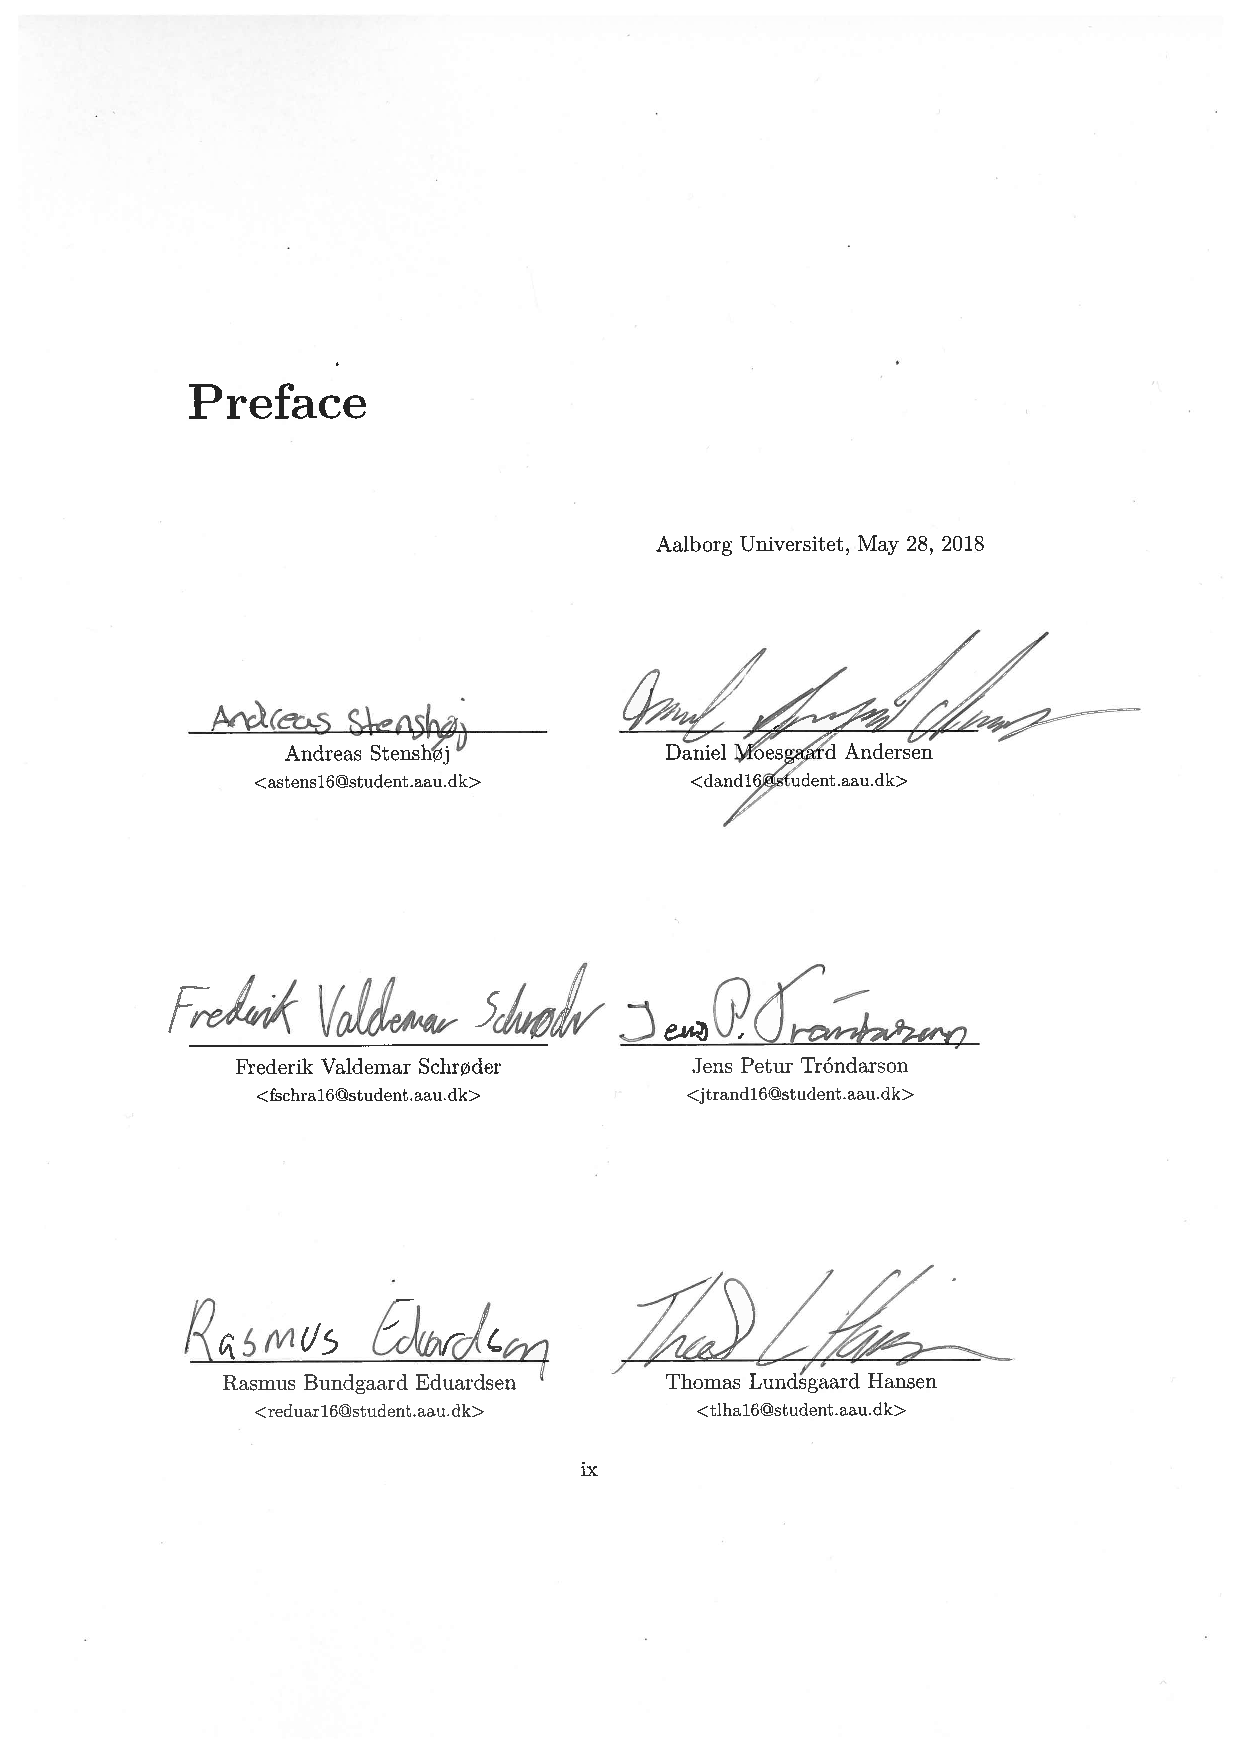
\includepdf[pages={1}]{Preface.pdf}
\cleardoublepage
%mainmatter
\pagenumbering{arabic} %use arabic page numbering in the mainmatter
\chapter{Introduction}\label{ch:Introduction}
Technology is constantly changing how we live our lives, do our work and interact with each other. One of the ways technology influences our everyday lives is through home automation. Home automation is becoming a bigger part of mainstream consumers lives due to it being a convenient way to automate certain tasks in the home that could be considered tedious. Some of the first to adapt to new technology are hobbyists \cite{TheHobbyistRenaissance}. The hobbyist uses the technology because of excitement and an interest in the subject, and not because of any professional reasons.
\\\\
The output of this project is a new programming language named PHAL, which is short for Personal Home Automation Language, which will help hobbyists build their home automation system, and a compiler designed to compile this new language to create usable programs. In order to accomplish this, this report will cover an initial problem analysis based on the topic of home automation, in which the necessary functions for home automation are considered. After the initial design considerations are concluded, the language analysis takes place where the language criteria and essential features are discussed and related to the target demographic, and finally some examples of PHAL code will be defined. 
\\\\
The report is split into five parts, each corresponding to a part in the process of crafting a compiler.
\\\\
In the \textit{Analysis} part, an analysis of the problem will be conducted where a platform will be chosen and the targeted users will be specified. The goal of part one is to get a clear understanding of the problem and how it can be solved.
\\\\
The second part, \textit{Designing PHAL}, deals with the definition of the PHAL language where we will delve into what it takes to develop a programming language and how the PHAL language should look.
The goal here is to define the requirements for the language, which will be done using the MosCoW model and give the reader an idea about the ideas that define PHAL.
\\\\
In the third part, \textit{Compiler design}, the language will be formally defined using context free grammars and we will delve further into what is required for creating a programming language in more technical terms.
\\\\
In the fourth part, \textit{Implementation}, the concrete implementations of PHAL will be explained using code examples. 
This part will include more information about how to generate an abstract syntax tree (AST), using ANTLR4 and how to later traverse this tree to analyse the code.
Likewise, it will delve into the construction of making a binding visitor, type checker and finally the code generation for PHAL.
\\\\
In the final part, \textit{Conclusion}, we will conclude on the results of this project, including a discussion about future work to further improve upon the PHAL language. 
\part{Analysis}
\chapter{Problem analysis}\label{ch:ProblemAnalysis}
In order to gain a deeper understanding of the problem domain, a problem analysis is conducted to scrutinise the underlying problems. In this chapter we define what \textit{Home Automation} is and which technologies are required, in order to get a deeper understanding of which features PHAL should support.

\section{Home Automation}
There are several different terms associated with computer controlled houses, such as 'Smart Home', 'Smart House' and 'Home Automation'. According to the book Smart Home Systems Chapter 1, Section 3, such a system is described as follows:
\begin{quote}
\textit{An automated home typically allows the control of room  luminosity,  opening  and  closing  of  shutters,  heating and  air  conditioning,  or multimedia systems. Home  applications  main  objective  is  the comfort  and simplification  of  the  daily  life  of residents,  and  home  support  of  elderly or  convalescents.}
\end{quote}
Following this definition, the more rigid definition, according to the EP1260886A2 patent (\cite{EP1206886A2}) is:
\begin{quote}
\textit{Home automation system \textit{(31}) comprising an array of functional devices \textit{(37)}, a plurality of input devices \textit{(38)} associated with the array of functional devices and a control unit \textit{(49)}, interconnected via radio link and constituting a home automation system \textit{(32)} \dots}
\end{quote}
Given these two definitions, anything electronic can, in theory, be included within a home automation system. This means that there are endless possible combinations as to what is connected to the systems. Due to this, PHAL will be focused on a narrow sub-part of home automation, due to the limited time and hardware at our disposal. This sub-part will be described later during this chapter, where only a small number of devices will be supported by PHAL.

\section{Platforms for home automation}
In the following section we will investigate the different hardware platforms suitable for creating a home automation system. We will take a more detailed look into the chosen platform and the current language thereto in order to gather information and find limitations in order to discover what can be improved in PHAL. 

\subsection{Choosing a platform}\label{PlatformsForHomeAutomation}
There are many different hardware platforms to choose from when creating a home automation system. Most of the available platforms are very similar in terms of hardware layout. However, they may differ in complexity and price. As seen on Table~\ref{tab:Platforms}, the major difference between the platforms is the price and the power voltage needed to operate the board.
\begin{table}[H]
\begin{center}
\begin{tabular}{|l|c|c|c|c|c|c|}
    \hline
    Name                                & Price     & Pins       & Output     & Memory      \\
                                        &           &            & power      &             \\\hline
    Arduino Uno R3 \cite{ArduinoUnoR3}  & 140 DKK   & 14         & 16 MHz     & 32 KB       \\\hline
    Raspberry Pi 3                      &           &            &            &             \\
    model B \cite{RaspberryPi3ModelB}   & 299 DKK   & 40         & 1.2 GHz    & 1 GB        \\\hline
    Intel Galileo \cite{IntelGalileo}   & 520 DKK   & 14         & 400MHz     & 256 MB      \\\hline
        Micro:bit \cite{MicroBit}           & 160 DKK   & 19         & 16MHz      & 256KB   \\\hline
\end{tabular}
\caption{The table shows the four different platforms and some of their pros and cons.}
\label{tab:Platforms}
\end{center}
\end{table}
\noindent
The price of a platform is essential in the decision making process when a hobbyist has to decide which platform to buy. If a given platform has similar specifications as other platforms, then the price is most likely going to be the deciding factor in which platform the hobbyist chooses to buy. 
\\
One of the things that limits the home automation systems which can be implemented using a given platform, is the native amount of pins available to connect input and output devices. It is therefore also important to consider this when choosing a platform.
\\
When creating a home automation system, the amount of calculations made by the control unit will presumably be relatively small, since it would only evaluate the input given to it in order to make a decision. Since a home automation system is not a time sensitive system the clock speed of the platform would not be significant when choosing a platform.
\\
When the platform receives information from its sensors and other input devices, the previous readings will typically not be stored in memory for long periods of time. Hence the memory available on the platform will not be significant when choosing a platform. 
\\\\
Based on the arguments listed above, the Arduino Uno platform has been chosen based primarily on its low price, which makes it an optimal match for hobbyists. Though the Arduino platform has a higher price per pin than the Raspberry Pi 3 model B, the Arduino can be extended with more general purpose input/output extension boards, providing a lower price per pin than the Raspberry Pi 3 model B.

\subsection{The Arduino platform}
Arduino is an open-source electronics platform, where the purpose of the platform is to make it easy to use hardware and software for educational purposes. 
The hardware of an Arduino is a circuit board which can read inputs from all sorts of different sensors such as ultrasound, light sensors or a temperature sensors connected to the female pins, which can be seen on Figure~\ref{fig:ArduinoUnoR3}. 
These can then be used in a program written for the Arduino, which in turn can produce different outputs. The output can, for example, be the ability to turn a light bulb on or off based on the input from the sensors. The instructions for Arduino are written in the Arduino Programming Language (APL) \cite{ArduinoLanguage}, which is based on the programming  languages C and C++. As a result of this, when the code is compiled it undergoes some changes, where the function calls are automatically generated in an intermediate language, afterwards the code is compiled with a C/C++ compiler called avr-g++ \cite{ArduinoLanguage}.
\begin{figure}[H]
\centering
  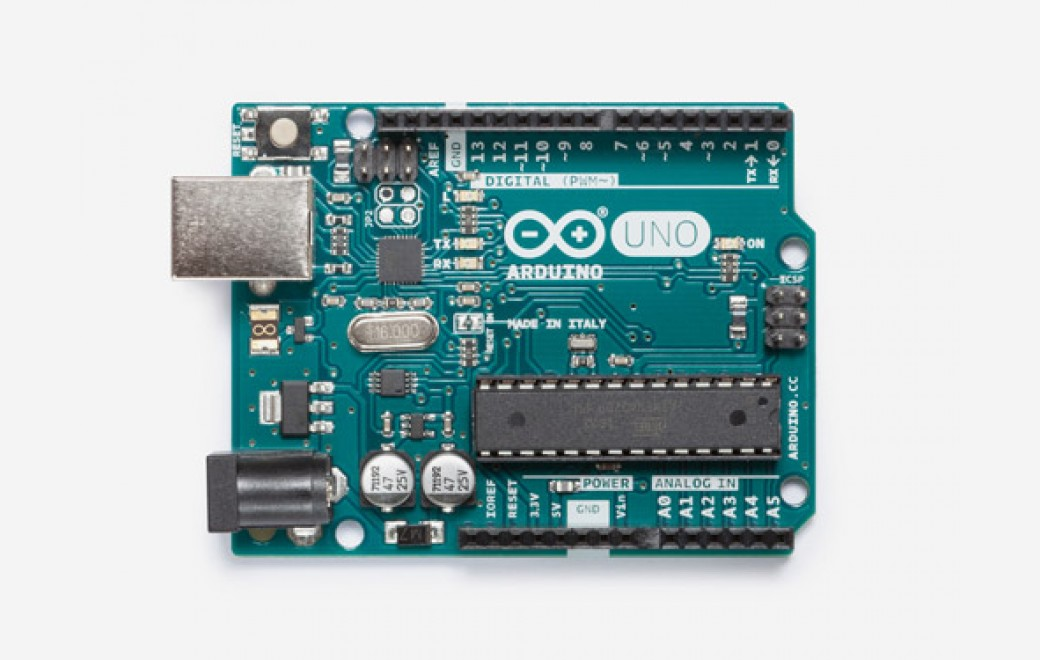
\includegraphics[width=\textwidth]{figures/Analysis/ArduinoUnoR3.jpg}
  \caption{This figure shows the Arduino Uno R3 board \cite{ArduinoUnoR3}.}
  \label{fig:ArduinoUnoR3}
\end{figure}
%\subsection{The use of Arduino}
\noindent
Arduino is designed to be easily accessible to all users, both experienced and inexperienced. The Arduino webside provides tutorials for beginners to learn how to program and use the language and platform. Furthermore, they have a dedicated community that is creating projects and sharing their experiences. The Arduino is inexpensive and readily available and would therefore be ideal for home automation projects due to its easy obtainability. Likewise, components for the Arduino are easy to obtain and are well documented on the internet which makes it ideal for the general hobbyist.

\section{Targeted users}\label{ProblemA:Users}
The intention with PHAL is to focus on the users with a limited amount of programming experience. Due to this, the language has to be intuitive and easy to understand and write. As mentioned in Subsection~\ref{ProblemA:ArduinoLanguage}, the Arduino is programmed in APL which is a c/c++ based language. APL inherits a lot of functionality from those languages, which makes it a powerful language, but not necessarily easily understandable.
\\\\
The focus of the PHAL language is to increase the level of abstraction for the user to create a much more simplistic and intuitive syntax, reducing the amount of programming knowledge needed to extract the full potential of the language when compared to APL. Because of the aim to reduce overall need of programming knowledge, the targeted users of our language are primarily hobbyists with no to little prior programming experience but some experience with electric circuits. 

\section{Technologies in a home}
In order to gain a deeper understanding of which technologies PHAL needs to support, an analysis of the technologies commonly used in a home automation system is conducted. 

\subsubsection{Lights}
The lights can be considered a basic element of any household. A light can be controlled in many different ways, such as by a button, light dimmer, through sensors or by timers. Given how essential lights are to a regular home, it is essential that the PHAL language needs the ability to control lights. This means PHAL should facilitate ease of using the lights through home automation \cite{BenefitsAndRisksOfSmartHomeTechnologies}.

\subsubsection{Heating systems and temperature sensors}
Roughly every home has some sort of climate control, such as radiators or heat pumps. An obvious use for a home automation system is as such to both monitor and control these aspects of the home \cite{BenefitsAndRisksOfSmartHomeTechnologies}.\\
Temperature sensors should logically be included as a supplement to heating systems, as a way of monitoring them.
\subsubsection{Motion sensors}
Motion sensors are one of the most dynamic ways to control devices in a home. It has the ability to sense if a person is in a room and turn the devices on or off accordingly. Motion sensors can also be used for other functionalities, and because of their wide range of use, are considered useful for the language to support \cite{BenefitsAndRisksOfSmartHomeTechnologies}.

\subsubsection{Motors}
For general purposes, motors can be included. Due to their simple functionality, they are easy to customise to perform a large variety of tasks, including moving objects such as windows or powering a fan.\\
Due to their level of usability diversity, motors are deemed essential for PHAL to support.

\section{Problems with the Arduino language}\label{ProblemA:ArduinoLanguage}
One of the primary annoyances with the Arduino language is the approach to setting up and using modules. Modules are hardware components that are connected to the Arduino via the pin ports on the board itself. In the Arduino language the pins are specified with the pinMode method, which can be seen on Listing~\ref{code:ArduinoExample}. This requires the user to specify whether the given pin serves as input or output \cite{FiveCommonArduinoMistakes}.
\\\\
It would be preferable to simply specify the given component and which pins it uses, and let the language automatically determine whether it is output or input. 
In addition to this it would be beneficial for inexperienced programmers to have explicit types for each module, making it easier to interact with it in a more natural way, instead of storing the component pin numbers as integers and using this for interaction.
\\
\begin{lstlisting}[caption={Example of Arduino code showing the use of \textit{pinMode} and \textit{digitalWrite} \cite{BeginningArduino}.},label={code:ArduinoExample}]
void setup()
{
  pinMode(13, OUTPUT);  // sets the digital pin 13 as output
}

void loop()
{
  digitalWrite(13, HIGH);   // sets the digital pin 13 on
  delay(1000);              // waits for a second
  digitalWrite(13, LOW);    // sets the digital pin 13 off
  delay(1000);              // waits for a second
}
\end{lstlisting}
In the example above, a small Arduino code example is shown. The \textit{setup} function is used for all declarations of variables, and the \textit{loop} function performs the logic for the Arduino, which in this case will switch on whatever component is connected to pin 13.
\\\\
Another concern with the Arduino language is the low level of abstraction it provides. Furthermore, it can be quite difficult to read what is going on in a program written in APL if you're unfamiliar with programming, and thus we wish to try and makes it more clear in PHAL. Exactly how PHAL will be solving these issues will be described in Chapter \ref{sec:PersonalHomeAutomationLanguage}.

\section{Problem specification}\label{sec:ProblemSpecification}
In this chapter, the problem domain has been analysed in order to get a greater understanding of what the problem is. Our conclusion is that APL has a level of complexity which is deemed unsuitable for our targeted users specified in Section~\ref{ProblemA:Users}. Because of this, the problem solved by this project is going to be:
\begin{quote}
Can we create a compiler for a new programming language for the Arduino platform, that will help novice users with limited prior programming experience create home automation systems?
\end{quote}
%Following the definition of a home automation system, it is necessary to further investigate the targeted users of PHAL. Due to the popularity and price of the Arduino platform, it is the optimal choice for creating a customised home automation system.
%\\\\
%However, the challenge of having to learn the Arduino Programming Language might scare away users who are not used to programming. Because of this, PHAL was chosen to focus on the hobbyists who would want an easy introduction to programming an Arduino for home automation, without having to learn the Arduino Programming Language. This means the targeted users are people interested in home automation but are inexperienced programmers.

\section{Summary}
In this part we have analysed what a home automation system is and what it can consist of. This will prove useful later on when defining the types within PHAL. The most used hardware platforms have been compared in order to determine which platform PHAL should be compatible with. Finally, The problems in the existing solutions for the Arduino platform have been analysed, and a problem specification has been formulated that should be solved with the PHAL language.

\part{Designing PHAL}
\chapter{Developing a language}\label{ch:TheCompiler}
In this chapter we will take a look at what needs to be done in order to create a language. First of all, a compiler needs to be built, and thus a short introduction to this will be presented together with how the syntax analysis is done for a language. Finally, we will examine the definition of the syntax and functionality of the language. 
\section{The compiler}
A compiler is essentially a program which takes a source code in one language as input, and then converts this to have the same properties in another target language as output. The compiler we are to build, must be able to compile programs written in PHAL into APL which will then be further compiled into a .hex file which is executable by an Arduino machine\cite{ArduinoBuildProcess}.
\subsection{Compilation phases}
When compiling a program, the source code has to go through a number of compilation phases before the target code can be generated. These phases consist of:
\begin{itemize}
    \item Scanning
    \item Parsing
    \item Creation of the abstract syntax tree (AST)
    \item Semantic analysis of the AST
    \item Traversal of the AST to generate translation
\end{itemize}
\begin{figure}[H]
\centering
  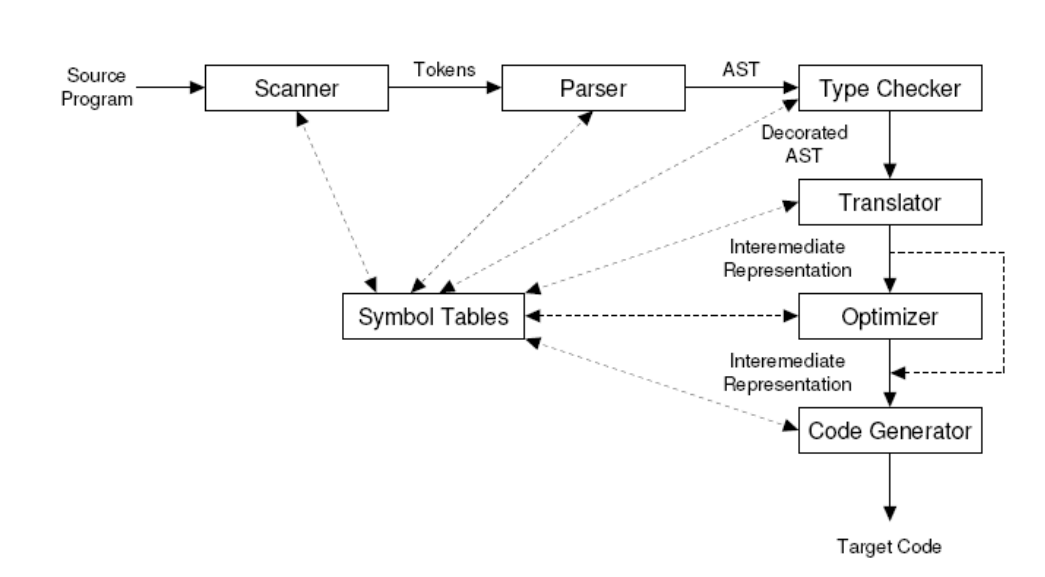
\includegraphics[scale=0.5]{figures/CompilerPhases/compilerPhases.PNG}
  \caption{This figure shows a syntax-directed compiler \cite{CraftinfACompiler}. }
  \label{fig:compilerPhases}
\end{figure}
\noindent
On Figure~\ref{fig:compilerPhases} the phases which the compilation process goes through is shown. Firstly, the source program written by a programmer in a specific language is used as input. This is then analysed, where each string of the input is scanned and sorted into different categories of strings called \textit{tokens}. These tokens are then syntactically analysed in the parser to check if the code submits to the rules defined in the grammar for the language. After the syntactic analysis has constructed the abstract syntax tree, as shown on figure \ref{fig:compilerPhases}, the semantic analysis takes place. During this phase the code is semantically checked, meaning that types and scopes are identified and defined. If the source code passes these different phases, the target code can be generated, which is the final phase of the compiler \cite{CraftinfACompiler}.
 
\section{Syntax analysis}
In this section we take a look at the different parts of the syntax analysis. The syntax analysis is the first part of the compilation phase, and it is responsible for making sure that the compiler can recognise the language that has been defined with the grammar. 
% Chapter 3 Fischer
\subsection{Lexical analysis - the scanner}
The scanner is responsible for looking through all of the characters in the source code and find tokens in the code. This is known as the lexical analysis, which is the first part of the syntax analysis. 
\\\\
The scanner will often be able to look a few characters ahead which helps determine what kind of token it is reading. If the scanner finds input that is not part of a defined token, it should show an error. The output of the scanner is a more compact version of the source code, which is represented as a stream of tokens. The scanner will simplify the job of the \textit{parsers} by eliminating the unneeded information, such as whitespace, and by sorting the source code into tokens \cite{CraftinfACompiler} rather than source code.
\\\\
\textbf{Tokens}
\\\\
Tokens are different categories of specific strings that have been sorted by the lexical analyser. A token can, for example, be identifiers, integers or reserved words. The reason that the string of characters which are input to the lexical analyser must be sorted into tokens, is to make it possible for the parser to check if the input is correctly written in relation to the defined grammar.
\\\\
\textbf{Regular expressions}
\\\\
The scanner needs a method to recognise which category of tokens the strings belong to. To do this, the scanner uses regular expressions to look for the tokens. Regular expressions describe the alphabet that a token consists of, and how the characters of the alphabet can be put together to form a string that belongs to this token. For example an integer is expressed as:
\begin{center}
    ( \{-\} ? \{1-9\} \{0-9\}* ) $\cup$ \{0\}
\end{center}
This regular expression shows that an integer can be preceded by zero or one \textit{"-"} which is indicated with the \textit{?} operator, followed by an integer between 1 and 9, and then zero or more integers between 0 and 9 which is indicated with the \textit{*}. The integer can also just be a single 0. Regular expressions for types in PHAL will be described further in chapter \ref{FormalDefinition}
\\\\
\textbf{Finite automata}\
\\\\
Regular expressions are a convenient notation for describing tokens in programming languages. This is due to regular expressions being able to be converted into nondeterministic finite state automatons (NFAs), which can be converted into deterministic finite state automatons (DFAs). This is useful as DFAs can be easily implemented as computer programs. 
\\\\
The finite state automaton is defined by Michael Sipser in the book \textit{Introduction to the Theory of Computation} as a 5-tuple consisting of the following:
\begin{itemize}
    \item \textit{Q} is a finite set called the \textit{states}
    \item $\Sigma$ is a finite set called the \textit{alphabet}, which is any non-empty finite set 
    \item $\delta$: $Q$ $\times$ $\Sigma \xrightarrow{}$ $Q$ is the \textit{transition function} which defines the rules for moving between states, where the domain of the function is the set $Q$ $\times$ $\Sigma$ and the range is $Q$
    \item $q_{0}$ $\in$ \textit{Q} is the \textit{start state}, meaning the start state is found in the set of states \textit{Q}
    \item \textit{F} $\subseteq$ \textit{Q} is the \textit{set of accept states}, meaning the set \textit{F} of accept states is a subset of \textit{Q} \cite{sipser}
\end{itemize}
Below is an example of a DFA:
\begin{figure}[H]
\centering
  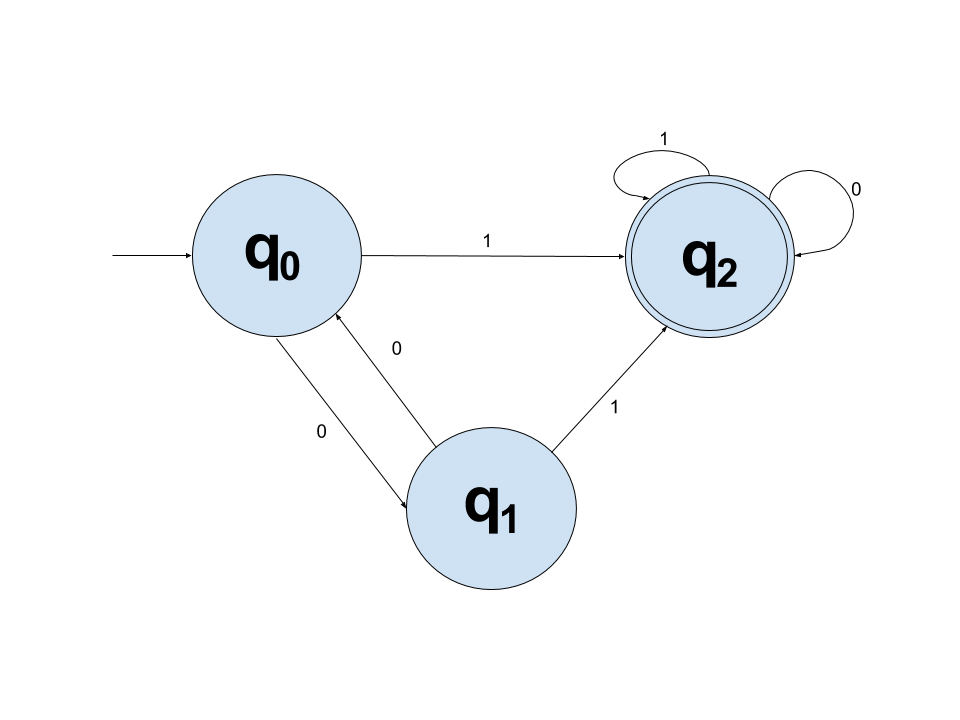
\includegraphics[scale=0.35]{figures/DFA.png}
  \caption{This figure shows an example of a DFA.}
  \label{fig:dfaExample}
\end{figure}
\noindent
In this example, the states are $Q = \{q0, q1, q2\}$, the alphabet is $\Sigma = \{0,1\}$, the start state $q_{0}$ is $q0$ and the accept state $F$ is $q2$. 
The arrows show how the automaton transitions from one state to another when it receives a given input. 
$q2$ is the accept state, this automaton accepts any string that contains a $1$ , no matter how many times it appears or where in the string it appears. 
This is shown by the transitions from states $q0$ and $q1$ to the accept state requiring a $1$, and the iterations in the accept state that do not allow the input to transition away from the accept state. 
This automaton is deterministic, as there is always only one choice for a transition to a new state for a given input. 
\\\\
In a non-deterministic finite automaton (NFA), it could be possible to choose two transitions from a single state with one input. 
For example in figure \ref{fig:dfaExample}, if the transition from state $q0$ to state $q1$ was defined by a transition requiring $1$ as input, the automaton would be able to transition to both state $q1$ and state $q2$, making it non-deterministic. 
\\\\
This ultimately means that the generation of a scanner is based on:
\begin{itemize}
    \item Regular expressions to describe the tokens to be recognised
    \item Finite state automatons as an execution model to which regular expressions are "compiled"
\end{itemize}
% Write more about regular expressions?

\subsection{Syntactic analysis - the parser}
% Chapter 4 FISCHER
The parser is the part of the compiler responsible for checking if the tokens that are provided by the scanner fit the grammar specification for the language. This is where the \textit{Context-Free-Grammar} (CFG) is introduced, because the parser has to check the syntax of the language using the CFG as reference. 

\subsubsection{Context-Free-Grammars}
Context-Free-Grammars are a set of grammar rules/productions that define the grammar of the language. 
A CFG consists of terminal and non-terminal symbols. 
Terminal symbols represent strings that can be derived to a token category. 
The non-terminal symbols all define a production on their right-hand-side. 
\begin{lstlisting}[caption={Example of an Context-Free-Grammer}, label={example:cfg}]
Prog    -> A B C
A       -> a
B       -> d e A
        |  b
C       -> c

\end{lstlisting}
On Listing~\ref{example:cfg} a short example of a CFG can be seen. 
The first rule says that a non-terminal symbol \textit{Prog} can be derived to the non-terminal symbols \textit{A B C}. 
Non-terminal symbols all start with a capital letter. 
\\
As seen on line 3 on Listing~\ref{example:cfg} the non-terminal \textit{B} has two productions, meaning it can either be derived to \textit{d e A} or \textit{b}.
Terminal symbols on the other hand can not derive further. 
It should be possible to create a sentence containing only terminal symbols which can then be replaced by tokens \cite{CraftinfACompiler}.
An example of this, using the CFG specified on Listing~\ref{example:cfg} is shown in Listing~\ref{example:cfgderive}.
On the final line it is seen that all non-terminals has been derived to terminal symbols.
\begin{lstlisting}[caption={Example of an Context-Free-Grammer derivation}, label={example:cfgderive}]
Prog
=> A B C                ( Prog  -> A B C )
=> a B C                ( A     -> a)
=> a d e A C            ( B     -> d e A)
=> a d e a C            ( A     -> a)
=> a d e a c            ( C     -> c) 
\end{lstlisting}

\subsubsection{Recursive descent}
Recursive descent is a simple parsing technique used for parsers. 
In recursive descent, each non-terminal from the CFG is a procedure. 
The procedure then examines the next token from the token stream, provided by the scanner, to evaluate which production should be used. 
If there is a non-terminal on the right-hand-side, the procedure calls the procedure for this particular non-terminal, and thus we have the recursive part of the technique, because the procedure goes through the derivation tree for the stream of tokens.
\\\\
For example, if we look at the short CFG shown on Listing~\ref{example:cfg}, the procedure for the non-terminal \textit{B} would be represented as shown in Listing~\ref{RD:Procedure}. 
\begin{lstlisting}[caption={Procedure for a recursive descent of the CFG productions}, label={RD:Procedure}]
procedure B()
  if ts.peek()= d
  then
    call match(ts,d)
    call match(ts,e)
    call A()
  else
    if ts.peek()= b
    then
      call match(ts,b) 
    else
      call error()
end
\end{lstlisting}
As seen on Listing~\ref{RD:Procedure}, the procedure for \textit{B} needs to look for which production is being used. 
If it peeks \textit{d} on line 2, it expects to see \textit{d} followed by an \textit{e}, and then calls the procedure for the non-terminal \textit{A}. 
Otherwise if it peeks a \textit{b}, the procedure expects the terminal token \textit{b} and nothing else. 
If what the procedure peeks are neither \textit{d} nor \textit{b} an error will be called.
\\\\
To complete the recursive descent parser, a procedure like this has to be written for each of the non-terminals in the CFG, where every possible production has to be considered.
\\\\
Once the lexer and the parser phases are complete, the compiler is able to recognise text that is written in the specified language in accordance with the grammar. 
These two phases are only responsible for the syntactical analysis part of the compilation. 
\\\\
The compiler still does not understand if the correct types are used for the various expressions for example. 
Type checking and code generation must still be done by the compiler before it can be considered complete.

\section{Contextual analysis}\label{comp:ContextualA}
%% Skrevet fra chapter 2.7
After the source code has been through the syntax analysis by the parser and the abstract syntax tree has been generated, it is time for the contextual analysis. In this phase the source code is checked for aspects that are not easily seen by the syntax analysis, such as checking that identifiers are declared before use, the scope of the variables and type-checking using a symbol table. 
\subsubsection{Symbol tables}
In many languages, it is a requirement that identifiers are declared before use. This is also a requirement in PHAL, and to enforce this requirement a symbol table is used. The symbol table is created by traversing the AST and looking for identifiers, which are then written to the symbol table along with their type. Other things that are usually stored together with the identifiers are their scope, their storage class and their protection properties.

\subsubsection{Type checking}
Type checking is part of the semantic analysis, and the symbol table is used to check for type consistency. 
%% type hierarchy?
Many languages have a type hierarchy where for example a float is considered \textit{wider} than an int, because an int can be represented as a float, but not the other way around. So converting an int to float is often done automatically, but a float number to int has to be done explicitly, because the number loses precision in the conversion.
\\\\
The general process known as type checking consists of traversing the AST bottom-up, meaning that it goes from the leaves of the tree to the root. There are different approaches that can be used to traverse the AST, and one that is often used is the \textit{visitor pattern}. This pattern can be used to determine what the calculated type of a statement is, based on what is in the AST. 

\subsubsection{Visitor pattern}\label{comp:VisitorPattern}
To traverse the AST, the visitor pattern can be used. 
The visitor is class that has different methods for each type of object it will visit during the traversal. 
The \textit{Visitor} class will often be used as the super class and the derived class will then override methods where extra functionality is needed.
%Each operation that can be used is implemented as a subclass of the general visitor class. 
\\\\
The nodes that are operated on accepts the visitor and calls back the appropriate type-specific method using themselves as the parameters. 
This means new operations can be added without modifying the object types, meaning you would implement a new visitor rather than changing the given class for the specific node. 
The visitors implement the operations and have one method for each type of node they visit. 
\\\\
Ultimately, this means the visitor pattern is the super class of classes such as \textit{TypeChecker} and \textit{CodeGenerator} that implement the \textit{Visitor} abstract class, and all the AST node classes have \textit{accept} methods that call back the appropriate method.

\subsubsection{Decorated abstract syntax tree}
The decorated abstract syntax tree (DAST) is the result of the contexual analysis. The DAST is an AST that is annotated with useful information, such as the position in the source code, which can be used for error reporting, and the types that will be used for the semantic analysis.
\\
After this, the final part of the compilation is the code generation of the target language. In the code generation phase the decorated abstract syntax tree is used to generate the correct instruction based on the types. 
\\
The individual phases will be further described in Part~III  about compiler design.
\chapter{Personal Home Automation Language}\label{sec:PersonalHomeAutomationLanguage}
As described in Chapter~\ref{ch:ProblemAnalysis}, the aim of this project is to develop a new programming language for the Arduino hardware platform that is intuitive to use for the users described in Section~\ref{ProblemA:Users}.
\\\\
In this section we will discuss the language criteria as defined by Robert W. Sebesta and relate it to the demographic of PHAL, and through these criteria determine the features that PHAL should support. We will investigate different programming paradigms to relate to the subject \textit{Home Automation}, and compare the definition of PHAL to the current Arduino language. Finally, we will show some code examples written in PHAL to show the syntax of the language.

\section{Initial design of the PHAL language}
When designing a new programming language for the Arduino, the first step is to determine which features the programming language should implement. This is an essential part of the early development, since it lays the foundation for the rest of the development.  

\subsection{Syntactical brainstorm}
To come up with new ideas for a language, we had each of the designers perform a series of assignments to brainstorm the syntactical format of the language. They would imagine a new language that they thought to be fitting to the demographic and construct some code examples as shown on Listing~\ref{code:InitialExerciseCodeWriting}. 
\begin{lstlisting}[caption={This listing shows how a designer imagined the new language to look like}, label={code:InitialExerciseCodeWriting}]
TempSensor temp_indoor = 1
TempSensor temp_outdoor = 2
WindowController window = 3
Radiator rad = 4

if(temp_indoor.reading < 20)
  until(temp_indoor.reading > 20)
    rad.increase()

if(temp_indoor.reading > 30)
  if(temp_outdoor.reading > 10 & temp_outdoor.reading < 30)
    until(temp_indoor.reading < 25)
      rad.off()
      window.open()

window.close()
\end{lstlisting}
This forced the designers to be creative, and it helped to see what the other designers thought the new language could look like, and which features they wished to include. The different language syntaxes were discussed, serving to create a foundation for a language based on compromises. The compromise of this exercise would end up determining the syntax of PHAL. 

\section{Language criteria}
In this subsection we will examine the language criteria proposed by Robert W. Sebesta in the book Concepts of Programming Languages \cite{Sebesta}. These criteria are used for evaluation in accordance with the targeted problem domain. Figure \ref{fig:LanguageCriteria} shows the different criteria. 

\begin{figure}[H]
\centering
  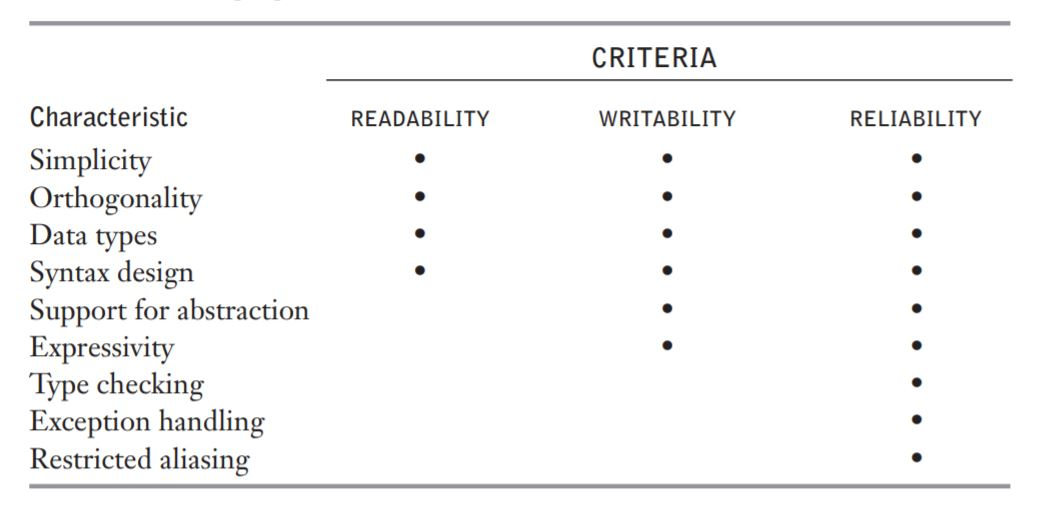
\includegraphics[scale=0.8]{figures/Analysis/sebestecriteria.JPG}
  \caption{This figure shows the language criteria proposed in Sebesta's book \cite{Sebesta}.}
  \label{fig:LanguageCriteria}
\end{figure}
\noindent
As shown, there are three major language criteria: readability, writability and reliability \cite{Sebesta}. The figure shows how the different characteristics affect them.
\begin{itemize}
    \item \textbf{Readability} pertains to the ease with which programs can be read and understood
    \item \textbf{Writability} is a measure of how easily a language can be used to create programs for a chosen problem domain
    \item \textbf{Reliability} relates to whether a program is able to perform to its specifications under all conditions
\end{itemize}
Since PHAL is targeted at users with limited programming experience as seen in Section \ref{ProblemA:Users}, and as such the language criteria valued the highest are the ones that we envision would help the demographic the most. These are simplicity, data types, syntax design, expressivity and type checking.

\subsection{Characteristics for language criteria}\label{subsec:CharacteristicsForLanguage}
In the following, the characteristics deemed relevant for PHAL will be described.

\subsubsection{Overall simplicity}
The overall simplicity of a language is tied to all of the main criteria, but strongly affects the readability of a language. This pertains to the amount of basic constructs contained in a language - more constructs mean it is harder to learn. This also relates to feature multiplicity, meaning multiple ways to accomplish the same goal should be avoided for simplicity. Operator overloading can also cause simplicity issues if used in excess of what is needed.
\\\\
This is especially relevant for PHAL. The language, as specified in Section~\ref{ProblemA:Users}, is targeted at hobbyists with a limited prior knowledge about programming. This means the language should aim to be as simple as possible for these programmers. PHAL should be comprised of few constructs, and these should be as easy to understand as possible to ensure simplicity. In accordance with the definition of simplicity, PHAL should include operator overloading where it makes sense while avoiding excessive use. The specific rules for overloading in PHAL will be discussed later in Section~\ref{subsec:FormalTypeRules}, where the type rules are discussed.

\subsubsection{Data types}
This relates to the ability to define data types and structures, and aids the readability of the program, for example through the use of \textit{true} and \textit{false} rather than $1$ and $0$.
\\\\
This is relevant for the same reasons as overall simplicity. PHAL needs to define data types that are as simple to use as possible, while giving the user the proper functionality required for home automation. The considerations made in regards to this, and the final types to be implemented are further discussed during the language definition in Chapter~\ref{ch:LanguageDefinitions}, and more in depth in the \textit{types} section, Section~\ref{Def:Types}.

\subsubsection{Syntax design}
This is the form of the elements of the language, which aids readability through use of intuitive keywords for the different tasks. 
\\
This is relevant for PHAL, as it is essential for all the major criteria. The language should be explicit in its syntax, and when performing operations an intuitive syntax should be ensured through relating the operations to general mathematical notation. The general syntax will be explained and used later in this report.

\subsubsection{Expressivity}
Expressivity means something can refer to several different characteristics. This relates to PHAL since the \textit{number} type is used for convenience rather than distinguishing between integers and floating point types.
On top of this, the language aims to be more expressive in its control structures, by adding keywords such as \textit{times} and \textit{until} in loops.

\subsubsection{Type checking}
The purpose of type checking is to test for type errors in a given program. Being able to identify these increases the reliability of the language. 
\\\\
\textit{Type checking} is highly valued for PHAL because of the demographic. It is expected that the programmers will make mistakes, and as such need to take appropriate action when it happens, and inform the programmer of what they did wrong in order to correct them.
\\
Type checking will be further described in technical terms in Chapter~\ref{ch:typechecking}.

\section{Programming paradigms}
In order to make a new programming language it is necessary to choose a programming paradigm for the language. 
A programming paradigm is a certain approach to computer programming based upon a set of principles and concepts, making each particular paradigm superior at certain kinds of problems.
\\
It is therefore important to discuss this subject and which of these paradigms should be used as a foundation for PHAL.
\\\\
Programming paradigms are also used to classify programming languages into certain categories based on their features. A programming language may feature more than one paradigm, such as C\#, which incorporates both the object oriented as well as the declarative paradigms. Below are some of the most common programming paradigms \cite{ProgrammingParadigmsKurtNormark}:
\begin{itemize}
    \item \textbf{The imperative paradigm} is based upon a \textit{first do this and next do this} approach. The order in which the commands are given is very important for the program to execute correctly. Commands can typically be assignments, input/output or procedure calls. This paradigm is rooted in the idea of the digital computer and how it functions. Some languages that represent this paradigm are C, Fortran, Algol and Pascal
    \cite{ProgrammingParadigmsDefinition}
    \cite{ProgrammingParadigmsKurtNormark}.
    
    \item \textbf{The functional paradigm} originates from a mathematical standpoint - the theory of functions. Kurt Nørmark describes the paradigm as: 
    \begin{quote}
        \dots it is considered by many to be a more clean version compared to the imperative paradigm because the imperative paradigm is based on the more complicated digital computer \cite{ProgrammingParadigmsKurtNormark}.
    \end{quote}
    In the functional paradigm, functions are first-class values which means they can be passed as arguments, modified, assigned to a variable and returned from a function. 
    Functions also work as the primary flow control, meaning that the functions decide how the program executes compared to other paradigms where an if-statement or other selective control structures implement this functionality. 
    This increases the written code's readability and maintainability since every single function is made to handle a specific problem and is not reliant on any external state. 
    The sequence in which the commands are given is also not important in this paradigm. 
    Some languages that use this paradigm are Lisp, Haskell, Erlang and F\# \cite{ProgrammingParadigmsDefinition} \cite{FunctionProgrammingVsImperativeProgramming}.
    
    \item \textbf{The declarative paradigm} is quite different from the other paradigms. 
    Instead of writing how to get what you want, you simply write what you want and it is then up to the compiler to figure out how to get it. 
    This paradigm is used extensively in query languages such as SQL and has also made its way into languages such as C\# with the addition of the LINQ library \cite{ProgrammingParadigmsDefinition} \cite{ProgrammingParadigmsForDummies}. 
    
    \item \textbf{The object-oriented paradigm} is based on the concept of \textit{objects} which may contain data and methods. 
    Some of the appealing aspects of the object oriented paradigm is the strong support for encapsulation and the very intuitive way of grouping together program aspects. 
    The objects are often made from classes, which act as a blueprint, where the objects are individual instances of its class. 
    A class can inherit from another class, this feature has multiple positive effects. 
    One of them is to reduce code duplication and it also enables message passing which reduces the amount of code needed to be written.
    Some of the languages that use this paradigm are C\#, Java and PHP \cite{ProgrammingParadigmsDefinition} \cite{ProgrammingParadigmsKurtNormark}.

    \item \textbf{The logic paradigm} is not a paradigm that is seen often in the more general areas of computation. 
    On the other hand, this paradigm works especially well when extracting knowledge from a given set of facts and relations. 
    This paradigm is rule based, but the rules do not need to be specified in a certain order. 
    It is simply up to the implementation to decide how these rules fit together to give the desired result. 
    This makes it a very proficient paradigm when working with artificial intelligence. 
    One of the most popular languages using the logic paradigm is Prolog \cite{Sebesta} \cite{ProgrammingParadigmsDefinition} \cite{ProgrammingParadigmsKurtNormark}.
    
    \item \textbf{The structured paradigm} is much like the imperative paradigm, but with a heavy emphasis on structures. 
    Structures are subroutines, conditions and loops and these are used to manage the control flow of the program, rather than using \textit{GOTO's} which were traditionally used very liberally \cite{ProgrammingParadigmsDefinition}.
\end{itemize}
When determining the proper paradigms to base PHAL around it is necessary to keep the targeted users in mind to choose an appropriate approach. 
As determined in Section~\ref{ProblemA:Users}, the language is aimed at users that want to do home automation on a hobby level, and is therefore required to be an introduction to programming and facilitate ease of use for new programmers.
\\\\ 
On top of this, the application of the language needs to be considered. 
PHAL is designed for home automation, and because of this, some approaches lend themselves better to this purpose. 
Some functionality of certain approaches could be considered redundant, especially in conjunction with the assumption that the users would write fairly simple programs. 
For this reason, the object-oriented, logic and functional paradigms are discarded. 
In our experience, it is preferable to have prior programming experience to fully grasp the concept of functions and classes which are core concepts in these paradigms. 
\\
Furthermore the logical paradigm does not seem to fit the problem domain which our programming language is supposed to cover. 
\\\\
As the target users are inexperienced, we feel that the most appropriate approach would be a mix of the imperative, structured and declarative paradigm. 
This allows the user to construct their program in an easy to comprehend manner using the imperative paradigm, while still using abstract yet easy to understand control structures as used in the structured paradigm. 
This also allows them to do more complex operations without having to write the code for it, using the declarative paradigm.

\section{The immediate goal of PHAL}\label{sec:phalvsarduino}
The main purpose of this project is to develop a more user friendly programming language for the Arduino hardware platform, as described in Chapter~\ref{ch:ProblemAnalysis}, compared to the default language provided for the Arduino. 
\\\\
One of the methods we plan on using to accomplish this is by adding a higher level of abstraction. This will make it easier for novice programmers to understand and use the PHAL language. 
This is done by combining some of the types from the Arduino Programming Language into types that are easier to work with for novice programmers, and introduce some new features such as \textit{groups}. 
In accordance with the intended demographic and avoiding the need for extensive programming knowledge, ending statements with the \textit{;} character seemed unnecessary and complicated. 
Instead we chose to use the separation of lines to end a statement, which means that every time the programmer creates a new line the previous statement is ended.
\\\\
\textbf{Numbers} in the Arduino language numbers are divided into multiple types. 
These are \textit{int}, \textit{byte}, \textit{double}, \textit{float}, \textit{long} and \textit{short}. 
For the intended users it is very hard to distinguish between the different types and know when to use them \cite{FiveCommonArduinoMistakes}. 
In PHAL all these types have been removed so the programmer does not need to decide on which type to use. 
Instead, a new type called \textit{number} will be introduced as the only type to handle numbers in PHAL. 
It is then up to the compiler to decide at compile time which underlying data type should be used instead.
\\\\
\textbf{Logical operators} in the Arduino language are implemented in a way that can be confusing for the intended users, such as for example the \textit{equal} operator being written as a double equal sign \textit{==}. 
This is easy to mistake by using a single equal sign, which specifies an assignment. 
For the intended user this is a very common mistake \cite{FiveCommonArduinoMistakes}. 
PHAL introduces a new operator - \textit{is}, which has the same functionality as the equal sign, and thus allows the user to use either of them.
\\
In the same way, the programmer will be able to interchangeably use words instead of mathematical operators for comparisons. 
The list of equivalent expressions can be seen on table~\ref{table:phaloperators}.
\begin{table}[H]
\centering
\caption{PHAL Operators} \label{LA:PhalOperators}
\label{table:phaloperators}
\begin{tabular}{|l|l|}
\hline
\textbf{Mathematical} & \textbf{Linguistic}        \\ \hline
=                   & is                               \\ \hline
!=                  & is not                           \\ \hline
\textgreater        & greater than       \\ \hline
\textless           & less than                      \\ \hline
\textgreater=        & greater than or equal to        \\ \hline
\textless=           & less than or equal to           \\ \hline
|                   & or                  \\ \hline
\&                 & and                 \\ \hline
!                    & not                 \\ \hline
\end{tabular}
\end{table}
\noindent
\textbf{Variable assignments} in the Arduino language are done using the single equal sign. 
To avoid ambiguity and ensure simplicity for the logical operators, the $=$ is replaced with the $:=$ operator in PHAL.
\\\\
\textbf{Strings} in the Arduino language are handled as \textit{char} arrays where the programmer needs to allocate the correct size of the array. 
The size cannot be changed afterwards. 
If the strings grow larger during the execution of the program a new \textit{char} array needs to be allocated by the programmer. 
This is a problem not only for the intended user, but also for programmers with prior experience \cite{FiveCommonArduinoMistakes}. 
PHAL will add a layer of abstraction to this issue. 
The programmer will have the ability to use a new type called \textit{text} that will be more like C\#, where the compiler will set the length of the \textit{char} array to make it easier for the programmer.
\\\\
\textbf{Structs} in Arduino language are used in the same way as structs in C, which the intended users have trouble with \cite{FiveCommonArduinoMistakes}. 
PHAL introduces a new datatype called \textit{group} which will attempt to make it easier for the programmer to group different data types together. 
It will also facilitate the ability to perform an action on all members of a group. 
\\\\
The considerations described and choices made in this section have all been based on the intention of making a language targeted at the intended users that Section~\ref{ProblemA:Users} defined, in an attempt to increase the simplicity of creating a home automation system for users using the Arduino platform.

\section{Examples of PHAL constructs}\label{ExamplesOfPHALConstructs}
To illustrate the considerations of PHAL's syntax, some coding examples for the different constructs will be established in the following section. 
The examples will consists of a listing showcasing the desired syntax, and a short explanation detailing the listing. 
In the following sections we will take a quick, informal view at the syntax for PHAL. 
\subsection{Comments}
\begin{lstlisting}[caption={Example of comments},label={code:comments}] 
# single-line comment
/* multi-line
comment */
\end{lstlisting}
For comments, a single-line comment will be preceded by a pound sign, this allows the user to enter comments in the code, that won't be handled by the compiler.
For multi-line comments, \textit{/*} will be used to indicate the start of a comment, and the reversed format \textit{*/} will be used to indicate the ending of that same comment. 

\subsection{Selective control structures}
The if statement serves as a structure that ensures that parts of the code are only executed when specific conditions are met.
\begin{lstlisting}[caption={Example of an \textit{If} statement},label={code:If-statement}]
if(<condition>) then {
  <statements and/or declarations>
}
else if(<condition>) then {
  <statement and/or declarations>
}
else then{
  <statement and/or declarations>
}
\end{lstlisting}
The \textit{if} statement is used to check if a specific condition is met. If this condition is met, the body inside the \{\} will be executed. Likewise, \textit{else if} is used to string multiple if conditions together. The following \textit{else if} condition will only be checked if the previous \textit{if condition} is not met. 
Finally, the \textit{else then} is used to execute code, but only if the previous \textit{if statement's} conditions are not met.
\\\\
The \textit{switch} statement serves as a simplistic alternative to the \textit{if-statement}. It allows the program to execute different statements, depending on the result of the expression. 
\begin{lstlisting}[caption={Example of a \textit{Switch} statement},label={code:Switch-statement}]
switch(<expression>) {
  case <n>:
    <statement and/or declarations>
  case <m>:
    <statement and/or declarations>
  default:
    <statement and/or declarations>
}
\end{lstlisting}
Unlike most programming languages, PHAL does not allow fall-through of switch cases. This means that the statement will automatically break whenever a case matches and finishes executing.
\\
The \textit{default} keyword works like the \textit{else} functionality of an \textit{if-statement}, and will only be executed if none of the previous conditions have been met.

\subsection{Loop}
For iterative control structures, it was decided to discard the usual \textit{for, while} and \textit{do while loops} and instead go with a more readable \textit{loop} structure. There will be different variations of the \textit{loop} structure, specifically \textit{loop x times} and \textit{loop until <condition>}. 
In the second version, \textit{increase by} and \textit{decrease by}, which can be seen on listing \ref{code:Loopstatement2}, are introduced to the syntax to help simplify the loops. 
Increase by and decrease by are optional parameters for the structure. \\
The following examples show the construction of loops:
\\
\begin{lstlisting}[caption={Example of a \textit{Loop} statement using until},label={code:Loopstatement1}]
loop until x > 100 {
  <statements>
}
\end{lstlisting}

\begin{lstlisting}[caption={Example of \textit{loop} statements using increase by and decrease by},label={code:Loopstatement2}]
loop until x > 100 increase x by 2 {
  <statements>
}

loop until x < 100 decrease x by 5 {
  <statements>
}
\end{lstlisting}

\begin{lstlisting}[caption={Example of a \textit{Loop} statement},label={code:Loopstatement3}]
loop x times {
  <statements>
}
\end{lstlisting}

\subsection{Methods}
Methods will be split into two separate listings, defining and calling. 
For defining methods, the keywords used are \textit{define, with} and \textit{returntype}. 
These keywords are introduced in an attempt to create context for the programmer. 
Defining a method will be done as shown on Listing~\ref{code:MethodDeclParam}:
\begin{lstlisting}[caption={Method declaration},label={code:MethodDeclParam}, escapeinside={(*}{*)}]
define <MethodName> with (<parameter1 type> <parameter1 name>, <parameter2 type> <parameter2 name>), (*\dots*)) returntype <returntype>{
  <content>
return <return value>
}
\end{lstlisting}
When defining a method that takes no parameters, a \textit{none} keyword is introduced:
\begin{lstlisting}[caption={Method declaration},label={code:MethodDeclNoParam}]
define <MethodName> with (none) returntype <returntype>{
  <content>
  return <return value>
}
\end{lstlisting}
When calling methods a \textit{call} keyword is used, and the \textit{with} keyword that was introduced for defining is still used. This would result in method calls looking similar to Listing~\ref{code:MethodCall1}:\\
\begin{lstlisting}[caption={Example of a \textit{method call} with parameters},label={code:MethodCall1}]
call <MethodName> with (<parameter1>, <parameter2>, <parameter3>)
\end{lstlisting}
When calling a method with no parameters, the \textit{none} keyword is used as seen on Listing~\ref{code:MethodCall2}.
\\
\begin{lstlisting}[caption={Example of a \textit{Method call} without parameters},label={code:MethodCall2}]
call <MethodName> with (none)
\end{lstlisting}

\subsubsection{The wait method}
PHAL will support some default methods to optimise the language for the problem domain and facilitate ease of use.\\
One of these will be the \textit{wait} method, which allows the user to make the Arduino wait for a given amount of seconds before continuing execution. An example of the syntax of the method can be seen on Listing~\ref{code:wait}\\ \begin{lstlisting}[caption={Example of the wait method},label={code:wait}]
wait 24.2 seconds
wait 2 seconds
\end{lstlisting}

\subsection{Including external libraries}
When using non-standard modules, eg. modules which are not natively supported by the language, external libraries can be included in the top of the file using the \textit{using} keyword followed by the library name as seen on Listing~\ref{code:includingLibrary}.  

\begin{lstlisting}[caption={Example of including an external library},label={code:includingLibrary}]
using <library name>
\end{lstlisting}

\section{Code examples}
On Listing~\ref{code:InitialSampleCode2} is an example of a program that has been created to demonstrate our thoughts for the language and how it could potentially look. 
Additional code examples can be found in Appendix~\ref{APP:examples}.

\begin{lstlisting}[caption={Sample code}, label={code:InitialSampleCode2}]
/*****************************************************
 * Program purpose:                                  *
 * The purpose of this program is to evaluate the    *
 * temperature within a room and increase the        *
 * temperature. If the temperature is too high, open *
 * a window using a motor.                           *
 *****************************************************/

setup {
  temperatureSensor tmp := pin 3, 2
  
  motor motorOpen := pin 5
  motor motorClose := pin 6
  
  number tmpLow := 19
  number tmpHigh := 26
}

repeat {
  if(tmp.reading greater than tmpHigh) {
    closeWindow(motorClose)
  } else if(tmp.reading less than tmpLow ) {
    openWindow(motorOpen)
  }
}

define openWindow with (motor open) returnType none {
  open := true
  wait 3 seconds
  open := false
}

define closeWindow with (motor close) returnType none {
  close := on
  wait 3 seconds
  close := off
}
\end{lstlisting}
Listing~\ref{code:InitialSampleCode2} shows the use of a temperature sensor and motor component. 
The temperature sensor is used to measure the temperature in a room. 
The temperature can be accessed by using the .reading modifier on the components as seen on line 22 and 14. 
The wait function is used to pause the program for an specified amount of seconds. 
In this listing it is used to ensure that the motors are turned of again after they have been running for 3 seconds. 

\section{MosCoW}\label{section:moscow}
To limit the scope of the project, the MosCoW method has been applied to keep the focus on the important matters of the project. 
The MosCoW method describes which aspects of the work is deemed a must for the project to be successful. 
Furthermore, it describes what the project should have but is not a main priority. 
Then, it describes what the project could have if time allows, and finally it describes what is deemed irrelevant for the project at this time, but that could be implemented later on were the project to continue. 
\\\\
The MosCoW for the project is as follows:
\\\\
\noindent\textbf{Must have:}
\begin{itemize}
    \item Setup - Repeat format
    \item Variables and control structures
    \item Ability to define and use functions
    \item Functional types:
    \begin{itemize}
        \item Number
        \begin{itemize}
            \item Has the ability to be a integer or a decimal number
        \end{itemize}
        \item Bool
        \begin{itemize}
            \item Have values of either true or false
            \item Use of the on and off aliases for true and false
        \end{itemize}
        \item Text
        \begin{itemize}
            \item Contains a sequence of characters
            \item Needs the ability to concatenate texts together with the $+$ operator
        \end{itemize}
        \item Component
        \begin{itemize}
            \item Ability to turn component types on and off
            \item Assigning pins to components without having to specify if it is an output or input pin
        \end{itemize}
    \end{itemize}
    \item Group type that groups components together
        \begin{itemize}
            \item Ability to apply a single operation to all members of the group
        \end{itemize}
    \item Lists
        \begin{itemize}
            \item Ability to group variables of the same type together
            \item Must be able to iterate through the content of a list
        \end{itemize}
    \item Support of light or LEDs
    \item Selective control structures
\end{itemize}

\noindent\textbf{Should have:}
\begin{itemize}
    \item Linguistic logical statements
    \item Ability to perform operations on groups
    \item Ability to read sensor components
    \item Iterative control structures
\end{itemize}

\noindent\textbf{Could have:}
\begin{itemize}
    \item Support of heating systems
    \item Support of motion sensors
    \item Ability to include libraries
    \item Some pre-programmed component libraries
    \item A reference keyword that allows parameters to be passed as a reference instead of value 
\end{itemize}

\noindent\textbf{Won't have (at this time):}
\begin{itemize}
    \item A complete library of components used in Arduino
    \item Ability to perform more complex operations on components that are specific to that component
\end{itemize}
\noindent
By including the points from the \textit{must have} part, a user will be able to write a minimalistic program that can control the light of the house, based on criteria controlled by a selective control structure.\\
With the \textit{should have} points, the user will be able to use additional hardware components, have further control of groups and the language will be expanded to reach a broader demographic unfamiliar with programming languages as defined in Section~\ref{ProblemA:Users}. These points were not deemed essential, but should be included in order for the language to be useful in a real-world context.\\
The \textit{could have} and \textit{won't have} points will further expand the amount of components that the user can use, by allowing the inclusion of external libraries and include further pre-programmed components. These are not necessary for the overall functionality of PHAL in regards to home automation, but are an obvious boon for the users if implemented.

\section{Summary}
With the goals and visions of PHAL in place, it is now possible to formally describe the language and the functionality hereof.
In the next chapter we will take a look at defining the syntax.
\part{Compiler design}
\chapter{Syntax definition}\label{ch:LanguageDefinitions}
In order for PHAL to be realised and to create a compiler to function as expected for the language, the language has to be defined. This is done through a combination of informal and formal definitions in the following chapter.

\section{Informal definition}
The aim for PHAL is to be relatively simple in comparison to other programming languages. 
It is intended for the Arduino hardware platform for home automation purposes, without needing extensive programming knowledge.

\subsection{Types} \label{Def:Types}
The programming language offers multiple data types:
\begin{itemize}
    \item The \textit{text} type consists of a sequence of characters.
    \item The \textit{number} type consists of a sequence of numbers. This type allows both integers and decimal values. 
    \item The \textit{bool} type is either \textit{true}, \textit{false}, \textit{on} or \textit{off}.
    \item The \textit{group} type is a complex type, consisting of multiple advanced data types.
    \item The \textit{list} type is a complex type, consisting of multiple elements of the same data type.
\end{itemize}
These types have been chosen in accordance with the considerations relating to the target demographic and the features discussed in Chapter~\ref{ch:ProblemAnalysis}.
The integer and float types found in languages such as C have been condensed into the single type called number, including both the floating point functionality and integer functionality. 
The \textit{text} type is functionally the same as the \textit{string} type found in languages such as C\#, but named more akin to what the users would use in their everyday speech for consistency in relation to the number type. 
\\\\
The bool type is maintained from languages such as C\#, where it is defined through the use of conditions that have the values true or false. 
When the name of the type was considered, candidates such as \textit{truthvalue} and \textit{boolean} were suggested, but the name was not changed as a suitable replacement was not found.
\\
As an extension to the regular usage of boolean values, PHAL will accept \textit{on} and \textit{off} as aliases for respectively true and false values.
\\\\
The group type allows grouping of multiple component types. 
An example of this could be kitchen appliances. 
Eg. a user has three lights in the kitchen, and wants them to automatically turn on at a specific time in the morning to facilitate waking up. 
In the language, the programmer would be able to combine these lights using the group type, creating an umbrella term for these lights - this could for example be a group named \textit{kitchenLights}. 
The programmer would then do automation on this group called \textit{kitchenLights} rather than each separate light one at a time. 
Another example would be starting a motor to open a window at the same time as the lights turn on - this could be accomplished in a group called
\textit{kitchenComponents} for instance. 
This means the group can also consist of multiple data types as well as nested groups.
\\\\
A list allows the user to group multiple elements of the same type together. 
The intended functionality of a list, compared to the group type, is that it allows the elements to be grouped together, but still be interacted with as individual elements.

\subsection{Keywords}
PHAL has a number of reserved keywords. 
The first set of keywords are related to selective control structures. 
As shown in Listings~\ref{code:If-statement} and \ref{code:Switch-statement}, we reserve the keywords \textit{if, then, else, switch, default} and \textit{case}. 
For \textit{if-statements} we combine the curly brackets of \textit{C} with the \textit{then} keyword for simplicity, and likewise the switches are kept in the style of \textit{C}, but without the need for a \textit{break} statement to avoid fall-through.
\\\\
For iterative control structures, shown in Listings~\ref{code:Loopstatement1}, \ref{code:Loopstatement2} and \ref{code:Loopstatement3}, we reserve the keywords \textit{loop, until, increase, decrease, by} and \textit{times}. 
These keywords are needed for the different loop variations, and are used in an effort to make loops simpler.
\\\\
Creating a function is done with the keywords \textit{define, with, none, return} and \textit{returnType} as shown on Listing~\ref{code:MethodDeclParam}. 
As seen on the listing, the \textit{with} keyword is used as a way of generating context in combination with the general parentheses notation for formal parameters of other languages. 
On top of this, the \textit{returntype} is defined after the parameters. 
In the body of the function the actual value returned is specified through the \textit{return} keyword.
\\
For calling functions we reserve the keywords \textit{call, with} and \textit{none}. 
As shown on Listings~\ref{code:MethodCall1} and \ref{code:MethodCall2}, the \textit{call} keyword is used for starting the call, and the \textit{with} keyword is used for the same reason as when defining functions. 
\\\\
For comparing statements the language reserves the use of mathematical operators. 
The demographic, even if they are not familiar with programming, are expected to be familiar with the mathematical operators \textit{<, >, <=, >=} and \textit{=}. 
On top of this, the language also allows the use of the following keywords \textit{or, is, and} and \textit{is not}. 
These keywords will replace the \textit{C} operators \&\& and || for simplicity.
\\\\
In terms of mathematical operators, the language reserves the use of the common algebraic operators \textit{+, -, /} and \textit{*}. 
These keywords will function the same as they do in mathematical operations. 
Finally, the \textit{+} operator will also be overloaded to serve as the operator for concatenating two strings when used on text variables.
\\\\
For the language we reserve certain keywords related to types as described in Subsection~\ref{Def:Types}. 
These keywords are \textit{text, number, bool, group} and \textit{list}. 
These keywords are reserved for definition of types for variables, and as such are not allowed for use outside of this.
\\\\
Parentheses and curly brackets are also reserved as apparent on the various listings cited in this section, mainly for use of encapsulating the different statements.

\subsection{Variables}
Variables are declared by specifying the variable's type prior to the name of it. 
PHAL allows variable names to consist of all letters from the roman alphabet.
\\
Variables are case-sensitive, but PHAL allows the user to use a variable without explicitly declaring it beforehand.
\\\\
For the naming of variables, we wish to have the variables start with a letter or an underscore, and the rest of the characters of the string can be either numbers, letters or underscores. 
The name of the variables cannot contain any other symbol except for numbers, letters and underscore.

\section{Formal definition} \label{FormalDefinition}
In this section we will describe the PHAL language with a formal definition. 
The informal definition generates a basic understanding but can be vague. 
The formal definition makes for a more precise representation of the language. 
We will for example present PHAL's CFG, regular expressions for PHAL and also the type rules.

\subsection{Lexemes and tokens}
In order to define the PHAL language we make use of lexemes and tokens. 
An input can be divided into these two categories, where lexemes are \textit{"words"} in the input, for example keywords, operators or identifiers. 
The token is a data structure for the lexemes and additional information. As a simple example for PHAL, the input \textit{a := 2 + 9.8} would be divided into lexemes and tokens in the following way:
\\
\textbf{Tokens:} id, assign, number, plus, number
\\
\textbf{Lexemes:} a, :=, 2, +, 9.8
\subsection{Token definition} 
All tokens with the exception of the keywords will be specified through regular expressions. 
Scanners are generally automatically generated through external software, where regular expressions are necessary because they are converted through algorithms.
The tokens for PHAL are described as follows:
\begin{itemize}
    \item Keyword
    \item Identifier
    \item Literals
    \item Operation
\end{itemize}
\subsubsection{Keywords}
A keyword can be one of the following:
\begin{center}
\begin{tabular}{c   c    c}
    and & bool & by \\
    call & case & decrease \\
    default & define & else \\
    for & group & if \\
    increase & is & list \\
    loop & none & not \\
    number & or & pin \\
    repeat & return & returnType \\
    setup & with & switch  \\
    text & then & times  \\
    until & &
\end{tabular}
\end{center}

\subsubsection{Identifiers}
Identifiers will be used for naming variables and classes. The identifiers must be formatted in such a way that they start with either an underscore or a letter, which can be followed by zero or more letters, digits or underscores.\\
As a regular expression, this would be expressed as $[\_a-zA-Z][\_a-zA-Z0-9]*$.
In addition to the format, they must be different from the reserved keywords mentioned above.


\subsubsection{Literals}
Literals are a notation for representing values in code. PHAL uses the following types of literals:
\begin{itemize}
    \item boolean-literal
    \item number-literal
    \item text-literal
\end{itemize}
\textbf{Boolean-literals}
\\
There are two boolean literal values: \textit{true} and \textit{false}. The type of a boolean-literal is bool.
These two values have a set of aliases \textit{on} and \textit{off}. These have the same functionality as the default boolean values, and are solely included for readability in context.
\\\\
\textbf{Number-literal}
\\
As per the definition of the \textit{number} type in PHAL in Section \ref{Def:Types}, the number-literal is a combination of integer-literals and real-literals.
\\\\
An integer literal is a string in the source code that is recognised as an integer by the lexical analyser. 
Integers can be any string made of a combination of $[0-9]+$. An integer literal can also have prefixes to represent a negative value.
\\\\
The real-literal is a string in the source code that is recognised as a float. Floats are of the form $[0-9]+.[0-9]+$ meaning that has the form of two numbers divided by a period. 
\\\\
\textbf{Text-literal}
\\
Text-literals are the strings in the source code encapsulated by quotation marks. A text-literal can be any combination of characters with the exception of a few characters. Something that should be addressed in the compiler is the problem that arises if a string contains other quotation marks, this is solved by simply disallowing the use of the quotation mark character in a text-literal. 


\section{Structural template}
The main structure of a PHAL program has two functions: A setup and a repeat function.
\\\\
The setup function is called when a program starts. 
It is for example used to initialise variables, set up modules and which pins they use or include libraries. It will only run once.
\\\\
The repeat function does as the name implies; repeats while the program is running. 
It is used to actively interact with connected components.
\\\\
Both of the primary functions are required, and do not return anything.

\section{Context free grammars}\label{sec:cfg}
In order to describe the language, a context free grammar is used. A context free grammar (CFG) is a set of recursive rewriting rules, that are used to generate patterns of strings.\\
Michael Sipser describes a CFG as a 4-tuple consisting of (V, $\Sigma$, R, S) where
\begin{itemize}
    \item \textit{V} is a finite set called the \textit{variables}
    \item $\Sigma$ is a finite set, disjoint from \textit{V}, called the terminals
    \item \textit{R} is a finite set of \textit{rules}, with each rule being a variable and a string of variables and terminals
    \item $S \in V$ is the start variable \cite{sipser}.
\end{itemize}

\subsection{BNF and Extended BNF}\label{subsec:bnfEbnf}
In order to formalise the context free grammar, Backus Naur Form (BNF) was created in the late 1950s by John Backus and Peter Naur. This form is used to describe the syntax of the language.\\
BNF uses abstractions for describing the syntactic structures. \\
For example doing an assignment in PHAL such as \textit{Number y := 12} would be given by:
\\\\
<assign> $\xrightarrow{}$ <var> := <expression>
\\\\
The extended version of Backus-Naur Form allows for writing a more compact syntax, using a set of symbols which can be seen on Table~\ref{table:ebnf} \cite{ISOIEC14977}. 

\begin{table}[H]
\centering
\begin{tabular}{@{}lc@{}}
\toprule
\textbf{Usage}   & \multicolumn{1}{l}{\textbf{Notation}} \\ \midrule
definition       & =                                     \\
concatenation    & ,                                     \\
termination      & ;                                     \\
alternation      & |                                     \\
optional         & [ \dots ]                             \\
repetition       & \{ \dots \}                           \\
grouping         & ( \dots )                             \\
terminal string  & " \dots "                             \\
terminal string  & ' \dots '                             \\
comment          & (* \dots *)                           \\
special sequence & ? \dots ?                             \\
exception        & -                                     \\\bottomrule
\end{tabular}
\caption{Table of Symbols for EBNF}
\label{table:ebnf}
\end{table}
\noindent
Any grammar defined in EBNF can also be represented in BNF. One of the main differences between BNF and EBNF is that BNF can only represent one rule in a line, whereas EBNF uses a terminating character to mark the end of a rule. In addition to this, EBNF includes mechanisms for defining the number of repetitions, comments etc.
The full EBNF for PHAL can be seen on Appendix~\ref{BFG:BNF}.

\subsection{Parser generator}
In order to create a parser, multiple approaches can be taken. It can either be written by hand, which is both tedious and error prone, or it can be generated using an existing parser generators. In the following part the aspects of the ANTLR4 parser generator will be examined, and LL($k$) grammars will be defined. 

\subsubsection{LL($k$) grammars}
A parsing procedure is associated with each nonterminal, meaning that a derivation must be accomplished through the application of one of the nonterminal's productions. To choose the appropriate production, the parser inspects the next $k$ terminal symbols in the input. This means the choice of production can be predicted on the next $k$ tokens of input, for some constant $k$ chosen before the parser is put to use \cite{CraftinfACompiler}. This is called the lookahead. An example of this could be $k = 1$, meaning the grammar is LL($1$). This means the grammar has productions that can be uniquely predicted for each nonterminal. \textit{LL} means it is a top-down from left to right parser utilising left derivation.\\
The idea of left derivation means that if the parser has multiple possible derivations, it will always choose to expand from the leftmost rule first.\\

\subsubsection{Approach used for PHAL}
As described in Section~\ref{ProblemA:Users}, the language is aimed at users unfamiliar with programming. In accordance with this, we do not expect them to write large programs requiring large amounts of power or efficiency. On top of this, we expect the users to make mistakes during their use of the language, this means error diagnostics should be valued highly in order to give meaningful error messages and help to the user. Based on these considerations, we have decided to implement our parser through a top-down approach as we value better performance and error diagnostics higher than power. We will therefore investigate the different options for LL parser implementation and decide on a final choice.

\subsection{Tools for parser generation}
Parsers and scanners can be generated through different programs. In this section we will discuss JavaCC, Coco/R and ANTLR as tools for generating a scanner and parser for PHAL.

\subsubsection{JavaCC}
\textit{Java Compiler Compiler} or just JavaCC is a parser generator that is implemented in Java. JavaCC is based on LL($k$) grammars and can be used with a variable lookahead which can be set by the user to create a recursive descent parser for a language. 

\subsubsection{Coco/R}
Coco/R is a compiler generator that takes a grammar on EBNF form and generates a scanner and parser for that grammar. The scanner works as a deterministic finite automaton. The parser is a recursive decent parser that can accept languages defined as LL($k$), where $k$ is a constant. There are versions of Coco/R for most modern programming languages such as Java, C\# and C++. 

\subsubsection{ANTLR}\label{ss:antlr}
\textit{Another Tool for Language Recognition}, or simply ANTLR, is a lexer and parser generator written in Java. It accepts a CFG without left recursion and generates an \textit{ALL(*)} parser. The \textit{*} symbol denotes that it uses a variable lookahead. This lookahead is $1$ as often as possible but will vary if needed. The initial \textit{A} in the name means \textit{Adaptive}, and this means grammar analysis is moved to parse-time \cite{AdaptiveLL(*)}.
\\\\
The output of ANTLR is a lexer and parser that uses a \textit{Concrete Syntax Tree} (CST) as its data structure. The CST has more information within its nodes than an \textit{Abstract Syntax Tree} and is thus much larger and may be cumbersome to traverse. Because of this, the CST produced by ANTLR should be converted to an AST to facilitate tree traversal in later phases of the compiler. 

\subsubsection{Choosing a parser generator}
ANTLR was chosen for parser generation for several reasons. 
First and foremost, it allows the usage of EBNF in its configuration file, which in turn makes the grammar more readable, since it is more compact than the regular BNF format. 
\\\\
In addition to the point mentioned in Subsection~\ref{ss:antlr}, ANTLR has a well-developed plugin for Eclipse, which includes intellisense.\\
On top of the perks for the developers, ANTLR allows LL($*$) grammars, which are more powerful than the LL($1$) and LL($k$) parsers.
\\\\
Finally, ANTLR allows the generation of both a parser, lexer and visitor. The visitor generated will be similar to the one described in Section~\ref{comp:ContextualA}.
\\\\
The major downside of using ANTLR is the need to manually convert the created CST to an AST. This downside is mitigated by the other factors described above, and therefore ANTLR was chosen as the tool for parser generation.
\chapter{Contextual Analysis}
During the contextual analysis phase the abstract syntax tree (AST) is traversed to check the semantics of the given program. This means both the  scope rules and type rules need to be checked for validity, and they will be defined in this following section.

\section{Abstract syntax trees}\label{ca:ast}
% Chapter 7 Fischer 
The AST is a data structure designed to be used in all activities after the syntactic analysis. This is done in order to spread functionality in the compiler to different components to increase maintainability and make it more understandable. The abstract syntax tree is similar to a parse tree, but has certain unnecessary details omitted. The AST consists of nodes. These nodes can be parents, children or siblings in relation to which node is currently being examined \cite{CraftinfACompiler}.
\\\\
To make an efficient AST structure, it should account for the following:
\begin{itemize}
    \item ASTs are typically constructed bottom-up, and should support tree construction from the leaves toward the root.
    \item The list of siblings is generated through recursive rules.
    \item Some nodes have a fixed number of children, and some can require a random amount. An example of a node requiring a fixed amount of children would be the addition operation, requiring two numbers to add together. An example of a node requiring a different amount of nodes would be a list, as the user defines how many elements they want the list to contain.
\end{itemize}
%Taking these considerations into account, each node in the tree has certain pointers to be able to traverse the tree effectively:
%\begin{itemize}
%    \item Each node points to the next sibling, and to its leftmost sibling.
 %    \item Each node points to its leftmost child.
%    \item Each node points to its parent.
%\end{itemize} \todo{Gør vi faktisk det her i vores AST?????????????!??!?}
\subsubsection{Design of the AST}
Since the AST is involved in most compiler phases, certain characteristics should be emphasised in the final design.

\begin{itemize}
    \item There should be enough information to unparse the AST, meaning the program should be able to be reconstructed.
    \item The implementation should be separated from the essential information within the AST to facilitate use in each of the compiler's phases.
    \item The different phases of the compiler will view the AST differently.
\end{itemize}
Finally, for reference we include a picture of a regular concrete parse tree and the AST for the same input. These can be seen on \ref{fig:syntax-AST}.

\begin{figure}[H]
\centering
  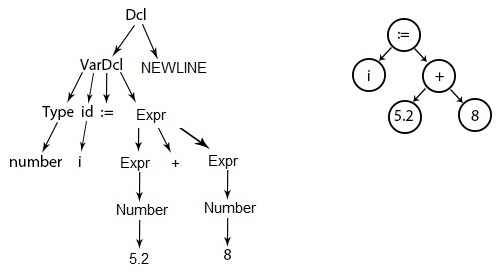
\includegraphics[width=0.8\textwidth]{figures/Syntax-AST.jpg}
  \caption{This figure shows the syntax tree (left) and AST (right) for the syntax \textit{number i := 5.2 + 8}.}
  \label{fig:syntax-AST}
\end{figure}


\section{Scope rules}
The scope rules of PHAL tell us which bindings are in effect under the execution of procedures. 
There are two kinds of scope rules which are dynamic and static.
Dynamic scope rules use bindings that are in effect when the procedure is called. 
This means that the scope is determined at run time.
\\\\
Static scope rules only use the bindings that where in effect when the procedure was declared. 
So the scope can already be determined at compile time.
We choose to use static scope rules in PHAL. 
The reasoning behind this is that we deemed static scope rules to be simplest to work with for the programmer. 
Static scope rules are also the most common scope rules for programming languages \cite{PilenVedTraeetsRod}. 
This means that if the programmer has any experience in programming then static scope rules will most likely be the most intuitive for them to work with. 
\\\\
For the functions in PHAL, we wish to have call-by-value, which means that when a variable is passed as an argument for a function, it is a copy of the variable's value that is parsed to the function.
\\\\
As described in the MoSCoW for PHAL, Section~\ref{section:moscow}, the implementation of a reference parameter will be considered, but not necessarily implemented. 
This allows the user to use pass by reference instead of pass by value.


\section{Formal definition}\label{Def:Semantics}
Once the informal definition of PHAL has been created, a formal definition needs to be formulated in order to remove any doubt about the behaviour of the language. 

\subsection{Syntactic categories}
The syntactic categories define the fundamental constructs of the language, and the elements in each category are represented by metavariables. These metavariables are defined in Table~\ref{tab:syntacticcategories}, and are used to ensure that it is clear when for example \textit{x, n, gx} or \textit{a} are variables that are already defined with a specific contextual meaning. Metavariables are different to regular variables. Regular variables could be defined as for example $y$, $z$, $obj$ or any other combination not present in the syntactic categories \cite{PilenVedTraeetsRod}. If multiple metavariables from the same category are present in a rule, they will be indexed - for example if two boolean expressions $b$ appear, they will be written as $b_1$ and $b_2$ respectively. 
\begin{table}[H]
\centering
\begin{tabular}{@{}lll@{}}
\toprule
Variable &       & Description                      \\ \midrule
$n$        & $\in$ & \textbf{Num} - Number                     \\
$x$        & $\in$ & \textbf{Var} - Variable                     \\
$gx$        & $\in$ & \textbf{GVar} - A variable of the group type                     \\
$lx$        & $\in$ & \textbf{LVar} - A variable of the list type                     \\
$\epsilon$ & $\in$ & \textbf{Epsilon} - The empty string \\
$new$      & $\in$ &  \textbf{Newl} - Newline                   \\
$a$        & $\in$ & \textbf{Aexp} - Arithmetic expression                    \\
$b$        & $\in$ & \textbf{Bexp} - Boolean expression                    \\
$adt$        & $\in$ & \textbf{Adv} - Advanced data type                     \\
$f$       & $\in$ & \textbf{FuncName} - The name of a function      \\
$S$        & $\in$ & \textbf{Stmt} - Statements               \\
$D_V$       & $\in$ & \textbf{VarDcl} - Declaration of a variable \\
$D_G$       & $\in$ & \textbf{GroupDcl} - Declaration of a group \\
$D_L$       & $\in$ & \textbf{ListDcl} - Declaration of a list \\
$D_F$       & $\in$ & \textbf{FuncDcl} - Declaration of a function \\
$D_{Adt}$       & $\in$ & \textbf{AdvDcl} - Declaration of an advanced type      \\
$D_P$       & $\in$ & \textbf{ParamDcl} - Declaration of parameters for a function \\
$P$       & $\in$ & \textbf{ParamOpt} - The parameter options \\
$Pin$      & $\in$ &  \textbf{Pins} - The pins that are used to connect the Arduino \\
$RTN$       & $\in$ & \textbf{Rtrn} - The returntypes \\
$P_S$        & $\in$ & \textbf{ProgStart} - The start of the program \\
$S_B$       & $\in$ & \textbf{SetBody} - The construction of setup      \\
$G_B$       & $\in$ & \textbf{GrpBody} - The body of the group \\
$L_B$       & $\in$ & \textbf{ListBody} - The body of the list \\
$L_T$       & $\in$ & \textbf{ListType} - The type of the list \\
$F_B$      & $\in$ &  \textbf{FuncBody} - The user defined function body  \\ 
$F_N$      & $\in$ &  \textbf{FuncNames} - The function names  \\
$L_N$      & $\in$ &  \textbf{ListNames} - The list names  \\
$G_N$      & $\in$ &  \textbf{GrpNames} - The group names  \\\bottomrule
\end{tabular}
\caption{Syntactic categories of PHAL}
\label{tab:syntacticcategories}
\end{table}
\noindent
These categories are necessary as we will be using the defined metavariable names within to construct an abstract syntax for PHAL.


\subsubsection{Abstract syntax for PHAL}
The abstract syntax describes the linguistic constructions of the language.
For every syntactic category the structure of the elements are described through a collection of construction rules, given in the form of context free production rules. 
These rules are seen for the categories in Table~\ref{tab:syntacticcategories}, with the exception of numbers $n$, variables $x$ and $newl$, because these are assumed to respectively be numerals, a collection of characters and the terminating character for lines in PHAL. 
Numerals in the context of semantics are defined as syntactic descriptions of numbers, so not actual numbers, but rather words for the numbers \cite{PilenVedTraeetsRod}. 
The category \textit{Epsilon} will only be detailed through rules in relation to a certain category of the abstract syntax. 
This category is the one concerning declarations, and it will be detailed in Section~\ref{subsec:declarations}.

\begin{table}[H]
\centering
\begin{tabular}{@{}lll@{}}
\toprule
Variable &       & Description                      \\ \midrule
$a$        & $::=$ & $n$ | $x$ | $gx$ | $lx$ | $a_1 + a_2$ | $a_1 - a_2$ | $a_1 * a_2$ | $a_1 \div a_2$ | $a_1 \bmod a_2$ | $ (a_1) $    \\
$b$        & $::=$ & $a_1 = a_2$ | $a_1 != a_2$ | $a_1 > a_2$ | $a_1 < a_2$ | $a_1 <= a_2$ | $a_1 >= a_2$            \\
            & & | $!b$ | $b_1$ \& $b_2$ | $b_1 | b_2$ | $(b_1)$  \\
            &&  | $a_1$ is $a_2$ | $b_1$ and $b_2$  | $b_1$ or $b_2$ |  $a_1$ is not $a_2$ | not $b$ \\
            &&  | $a_1$ greater than $a_2$  |  $a_1$ less than $a_2$  | $a_1$ less than or equal to $a_2$  \\
            &&  | $a_1$ greater than or equal to $a_2$ \\
            & & | true | false | on | off \\
$P_S$      & $::=$ & setup $S_B$ repeat $S$ $D_F$\\
$S_B$    & $::=$ & $S_B$ \textit{new} $S_B$ | $Dv$ | $D_G$ | $D_L$ | $D_{adt}$ | $S$\\ 
$S$        & $::=$ & $x:= a$ | $x:= b$ | $x \text{ += } x$ | $x \text{ += } a$ | $x \text{ -= } x$  \\
           & & | $x \text{ -= } a$ | $gx := b$ | $S_1 \textit{new} \: S_2$ | if $b$ then $S$ $S_{if}$ | if $b$ then $S$ \\
           & & | loop $S$ until $b$ | loop $S$ until $b$ increase $x$ by $n$  \\
           & & | loop $S$ until $b$ decrease $x$ by $n$ | loop $S$ $a$ times \\
           & & |  call $f$ with $y...y_n$ | call $f$ with $a...a_n$  \\
           & & | switch($a|b$) case $<a_1|b_1>: \: S_1$ $...$ case $<a_n|b_n>: \: S_n$ default: $S$ \\
           &&  | get element $n$ from $lx$ | remove element $n$ from $lx$  \\
           &&  | add $a$ to $lx$ | add $b$ to $lx$ | $\text{wait for } a \text{ seconds}$  \\
$S_{if}$     & $::=$ &  else if $b$ then \{$S$\} | else if $b$ then \{$S$\} $S_{if}$ |  else \{$S$\} \\
$D_V$       & $::=$ & $var$ $x := a \: \textit{new}$ $D_V$ | $var$ $x := b \: \textit{new}$ $D_V$ | $\epsilon$ \\
$D_G$       & $::=$ & group $gx$ $G_B$ \textit{new} $D_G$ \\
$G_B$      & $::=$ & adt x \textit{new} $G_B$ | group gx \textit{new} $G_B$ | $\epsilon$ \\
$D_L$     & $::=$ &  list $L_T$ $lx$ $L_B$ \textit{new} $D_L$ \\
$L_T $     & $::=$ &  group | number | bool | text | motor | temperatureSensor | lightbulb\\
$L_B $     & $::=$ &  $a$, $L_B$ | $x$, $L_B$ | $gx, \: L_B$ | $b, \: L_B$ | $a$ | $x$ | $gx$ | $b$ | $\epsilon$ \\
$D_F$       & $::=$ & define $f$ with $P$ $F_B \: \text{returnType} \: RTN \: \textit{new}$ $D_F$ | $\epsilon$ \\
$P$ & $::=$ & none | $D_P$ \\
$D_P$  & $::=$ & var x, $D_P$ | group gx, $D_P$ | adt x, $D_P$ | list lx, $D_P$ | var x \\
            & & | group gx | adt x | list lx  \\  
$RTN$       & $:=$ &  none | number | text | bool | group | list | adt\\
$F_B$       & $:=$ &  $F_B$ \textit{new} $F_B$| $D_V$ | $D_P$ | $D_G$ | $D_L$ | $S$ | $S_{wait}$ | return $x$\\
$D_{Adt}$   & $::=$ & $adt$ $x$ $:=$ pin $Pin \: new \: D_{adt} | \: \epsilon  $  \\ 
$adt$   & $::=$ & motor | temperatureSensor | lightbulb     \\ 
$Pin$       & $::=$ & $ n, Pin$ | $n$ \\
\bottomrule
\end{tabular}
\caption{Abstract syntax of PHAL}
\label{tab:syntacticformation}
\end{table}
\noindent 
\subsection{Environment-store-model}\label{semantics:EnvStore}
In order to formally define the semantic rules for PHAL we will construct big-step-operational semantic rules for the language. 
This will be done through the \textit{environment-store-model}. This model is used to describe how variables are bound to values through what is called a \textit{variable environment} and a \textit{storage}. 
Variables are bound to a location address, and each location address is bound to a value. 
This value is then the value of the variable that points to that location. 
As such, the \textit{environment-store-model} describes both the locations in memory and which values are stored there.
A visual representation of the model can be seen on Figure~\ref{fig:ESModel}.
\\\\
The variable-environment is essentially a symbol table containing the variable and the address. 
The \textit{storage} describes which values are found at the different storage locations, by defining the value and storage connection \cite{PilenVedTraeetsRod}. 
The values stored in storage can either be numbers, text, booleans or advanced data types.
\\
Figure~\ref{fig:ESModel} gives an illustration of this, where the variables describe a location, and the location describes the storage. 
The variable table contains a \textit{next} variable, that points to the next unused location. 
\begin{figure}[H]
\centering
  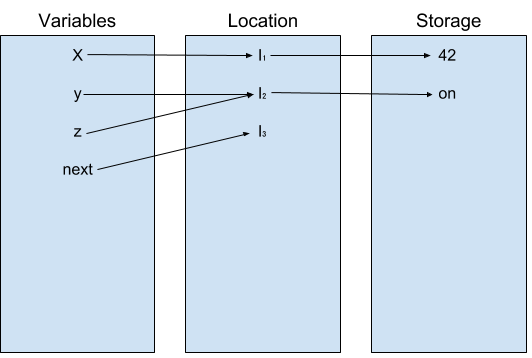
\includegraphics[width=0.7\textwidth]{figures/semantics/1.png}
  \caption{This figure shows an example of the Environment-Store Model.}
  \label{fig:ESModel}
\end{figure}


\noindent
The set of variable-environments is the set of partial functions from the variables to the locations, denoted $EnvV$. 
A single element of $EnvV$ is defined as $env_v$. $EnvV$ is defined as such:
\begin{equation*}
\centering
    EnvV = Var \cup next \rightharpoonup Loc
\end{equation*}
This means the variable environment is a list of variables and a next variable that all point to a location.
\\\\
 The set of possible storage locations is denoted $Loc$. Locations are assumed to be of the set of integers, as this is satisfactory for the purposes with which the model will be used in this section. This means the locations are defined as \\ 
\begin{equation*}
\centering
    Loc = \mathbb{Z}
\end{equation*}
\\
The set of storage values is the set of partial functions from location to values, defined as:
\begin{equation*}
Sto = Loc \rightharpoonup Number \cup Text \cup Bool \cup Adt
\end{equation*}
This means that each element in the list of locations point to a value in storage that is typed as either a number, text or bool. 
A single element of $Sto$ is defined as $sto$. 
\\\\
These sets are defined through partial functions because it is not necessary to explain the location of every single variable imaginable, but rather just the ones that are used.

\subsection{Transition systems}
Defining operational semantics is done by defining a transition system. The transition system is an oriented graph, where the edges are equivalent to a step of a program and the vertices represent a snapshot of the program \cite{PilenVedTraeetsRod}. In operational semantics, the edges are called transition and the vertices are called configurations. Vertices without outgoing edges are called the ending configurations. The transition system is then defined as the following triple:
\\
\begin{equation*}
\centering
    (\Gamma, \xrightarrow{}, T)
\end{equation*}
$\Gamma$ is a set of configurations, $\xrightarrow{}$ is the transition relation and $T$ is a subset of $\Gamma$, denoting the ending configurations.
To further illustrate, a finite transition system is shown in the following figure:
\begin{figure}[H]
\centering
  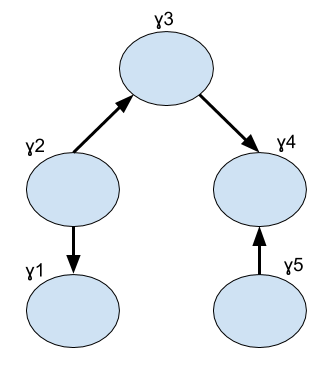
\includegraphics[width=0.4\textwidth]{figures/semantics/TransistionssystemsFigur.png}
  \caption{An example of a transition system}
  \label{fig:TransistionSystem}
\end{figure}
\noindent
On Figure~\ref{fig:TransistionSystem}, the possible configurations $\Gamma$ is the set $\{\gamma1, \gamma2, \gamma3, \gamma4 \text{ and } \gamma5\}$. The transition relation is given through pairs $(\gamma, \gamma')$, denoting that there is a transition from $\gamma$ to $\gamma'$. For the example, the transition relation is then: 
\begin{center}
$\xrightarrow{} \: = \{(\gamma2, \gamma1),\: (\gamma2, \gamma3), \:(\gamma3, \gamma4), \:(\gamma5, \gamma4)\}$
\end{center}
The ending configurations have no outgoing transitions, and thus for the example the set $\{\gamma1, \: \gamma4\}$ makes up the ending configurations $T$.

\subsection{Reading structural operational semantic rules}
Big step semantic rules are constructed using premises, conclusions and side conditions. 
The general shape of a rule is that, given one or more environments and a store, the premises of the rule specifies how the conclusion reaches the result of modified environments and a modified store.
\\\\
In addition to the premise and conclusion, the rule can make use of a side conditions to define for which cases the conclusion holds. An example of the setup of a rule would be like this:
\begin{equation}\label{EQ:exampleSemantic}
\cfrac
{
    environment, \: store \vdash \: Premise \xrightarrow{} updated \: env \: and \: sto
}
{ 
    environment, \: store \vdash Conclusion \xrightarrow{} updated \: env \: and \: sto
}
\quad side \: condition
\end{equation}
The $\vdash$ operator shown before the premise and the conclusion describes what knowledge you need to properly define the rule. 
So for this example, in order to reach the conclusion, knowledge of both the current environment and the current store would be necessary. 
An introductory example constructed for PHAL, including all the elements of a semantic rule, would be the rule for adding numbers together as shown on Equation~\ref{EQ:SemainticsArithmeticExprPLUSNumber}
\begin{equation}\label{EQ:SemainticsArithmeticExprPLUSNumber}
\begin{minipage}{.2\linewidth}
$[\text{PLUS-num}_\text{BSS}]$
\end{minipage}
\begin{minipage}{.8\linewidth}
\centering
$\cfrac{env_v, \: sto \vdash a_1 \xrightarrow{}\textsubscript{a} \: v_1 \quad env_v, \: sto \vdash a_2 \xrightarrow{}\textsubscript{a} \: v_2}{env_v, \: sto \vdash a_1 + a_2 \xrightarrow{}\textsubscript{a} \: v}$
$ \: where$ $v$ $=$ $v_1$ $+$ $v_2$
\end{minipage}
\end{equation}
The semantic rule shown on Equation~\ref{EQ:SemainticsArithmeticExprPLUSNumber} looks similar to Equation~\ref{EQ:exampleSemantic}, with the main difference being the premises. 
There are multiple premises in the PLUS rule, and they do not lead to an updated environment or store. 
This is common for rules concerning expressions, whereas the one explicitly shown on Equation~\ref{EQ:exampleSemantic} is more common for statements and declarations. 
This is due to expressions by themselves not affecting the environments or storages - in the case of PLUS, it merely computes the value of the addition of the two numbers. 
Declarations update environments because they save information about a declaration, meaning the environment containing that declaration will be different after the execution of the declaration. Statements change values based on context, meaning they can cause changes in the values in storage, thereby updating it.
\\\\
Equation~\ref{EQ:SemainticsArithmeticExprPLUSNumber} states that when the variable environment and storage are known, the statement $a_1 + a_2$ can be evaluated to a value $v$ if $a_1$ can be evaluated to a value $v_1$, and $a_2$ can be evaluated to a value $v_2$, when they meet the requirement specified in the side condition that states that $v = v_1 + v_2$. 
The arrows that appear in both the premises and the conclusion indicate that the evaluation of these values must be done through the transition relation for arithmetic expressions. 
This means that they must be evaluable through one of the transitions defined for arithmetic expressions. The full list of these is contained in Appendix~\ref{AppSec:SemainticsArithmeticExpr}.
\\

\subsection{Semantic rules of PHAL}
Using the big step semantic rules described, the semantic rules of PHAL can be described.
\subsubsection{Arithmetic expressions}\label{sem:aexp}
In the following subsection a small selection of the semantic rules for arithmetic expressions is shown and described, the full list can be seen in Appendix~\ref{AppSec:SemainticsArithmeticExpr}. 
The semantic rules for arithmetic expressions are based on the transition system 
\begin{equation*}
(\textbf{Aexp} \cup \; \mathbb{Q}, \: \xrightarrow{}\textsubscript{a}, \: \mathbb{Q})    
\end{equation*}
In the system, the possible configurations $\Gamma$ are given as all the possible expressions given by \textbf{Aexp} defined by the metavariable $a$ in the syntactic categories in Table~ \ref{tab:syntacticformation}, the transition relations $\xrightarrow{}\textsubscript{a}$ are given by the rules defined in Appendix~\ref{AppSec:SemainticsArithmeticExpr}, and the ending configurations $T$ are a subset of all possible configurations.
\\\\ 
In this case $T$ is given as the final value of an arithmetic expression $\mathbb{Q}$, as they are values and have no outgoing transitions.

\begin{equation}\label{EQ:SemainticsArithmeticExprPLUSText}
\begin{minipage}{.2\linewidth}
$[\text{PLUS-text}_\text{BSS}]$
\end{minipage}
\begin{minipage}{.8\linewidth}
\centering
$\cfrac{env_v, \: sto \vdash a_1 \xrightarrow{}\textsubscript{a} \: v_1 \: \: \: env_v, \: sto \vdash a_2 \xrightarrow{}\textsubscript{a} \: v_2}{env_v, \: sto \vdash a_1 + a_2 \xrightarrow{}\textsubscript{a} \: v}$
$ \: where$ $v$ $=$ $v_1$ $\circ$ $v_2$
\end{minipage}
\end{equation}
On Equation~\ref{EQ:SemainticsArithmeticExprPLUSText} the semantic rule for concatenating two strings can be seen. The rule states that when the variable environment and storage are known, the statement $a_1 + a_2$ can be evaluated to a value $v$, but only if $a_1$ can be evaluated to a value $v_1$ and $a_2$ can be evaluated to a value $v_2$, and the value of $v$ is the value of $v_1 \circ v_2$, as specified in the side condition.
\\\\
For the next rule, a function to convert from the syntactic description of numbers as numerals to actual numbers. This function is defined as:
\begin{equation*}
    \mathcal{N}: Num \xrightarrow{} \mathbb{Q}
\end{equation*}
$\mathbb{Q}$ denotes the set of rational numbers, meaning it allows for both integer values and decimal point values of numbers.
\begin{equation}\label{EQ:numbss}
\begin{minipage}{.2\linewidth}
$[\text{NUM}_\text{BSS}]$
\end{minipage}
\begin{minipage}{.8\linewidth}
\centering
$env_v, \: sto \vdash n \xrightarrow{}\textsubscript{a} \: v$ $ \: \text{if}$ $\mathcal{N}[\![n]\!]$ $=$ $v$ 
\end{minipage}
\end{equation}
The semantic rule shown on Equation~\ref{EQ:numbss} shows how a number is evaluated to an actual value from its syntactic representation. The rule states that when the variable environment and storage is known, a number $n$ can be evaluated to a value $v$ through use of the function $\mathcal{N}$.
\\
\begin{equation}\label{EQ:SemainticsArithmeticExprVAR}
\begin{minipage}{.2\linewidth}
$[\text{VAR}_\text{BSS}]$
\end{minipage}
\begin{minipage}{.8\linewidth}
\centering
$env_v, \: sto \vdash x \xrightarrow{}\textsubscript{a} \: v$ $ \quad \text{if} \quad env_v \: x = l$ and $sto \: l = v$ 
\end{minipage}
\end{equation}
On Equation \ref{EQ:SemainticsArithmeticExprVAR} the rule for evaluating variables is shown. The rule states that when the variable environment and storage is known, a variable $x$ can be evaluated to a value $v$, if the terms of the side conditions $env_v \: x = l \quad \text{and} \quad sto \: l = v$ are met. This means that the variable environment points $x$ to a location, and that the storage of that location $l$ points to the value $v$. First the location is found, and then the value contained in that location is determined.



\subsubsection{Boolean expressions}
In the following section a small selection of the semantic rules for boolean expressions is shown and described, for the full set of semantic rules see Section~\ref{AppSec:SemainticsBooleanExpr}.
Boolean expressions evaluate to either true or false, written as $tt$ and $ff$ respectively. The transition system for boolean expressions, \textit{Bexp}, is thus:
\begin{equation*}
    (\textbf{Bexp} \cup \{tt, ff\}, \xrightarrow{} \textsubscript{b}, \{tt, ff\})
\end{equation*}
The transition relation $\xrightarrow{}\textsubscript{b}$ is defined in Appendix~ \ref{AppSec:SemainticsBooleanExpr}. Some of the rules for boolean expressions require the evaluation of arithmetic expressions, and to do this the transition relation $\xrightarrow{}\textsubscript{a}$ is used as defined in Subsection~\ref{sem:aexp}.

\begin{equation}\label{EQ:SemanticsBooleanExprEQUALS}
\begin{minipage}{.2\linewidth}
$[\text{EQUALS-1}_\text{BSS}]$
\end{minipage}
\begin{minipage}{.8\linewidth}
\centering
$\cfrac{env_v, \: sto \vdash a_1 \xrightarrow{}\textsubscript{a} \: v_1 \quad\: env_v, \: sto \vdash a_2 \xrightarrow{}\textsubscript{a} \: v_2}{env_v, \: sto \vdash a_1 = a_2 \xrightarrow{}\textsubscript{b} \: tt}$
$ \: if$ $v_1$ $=$ $v_2$
\end{minipage}
\end{equation}
On Equation~\ref{EQ:SemanticsBooleanExprEQUALS} the rule for evaluating logical equals can be seen. The rule specifies that knowing the variable environment and the storage, the expression $a_1 = a_2$ can be evaluated to $tt$ if $a_1$ and $a_2$ can evaluate to values $v_1$ and $v_2$ through the transition relation $\xrightarrow{} \textsubscript{a}$, and the side condition of the rule is met. The side condition simply specifies the stipulation that the two values must be the same for the conclusion to be reached.

\begin{equation}\label{EQ:SemanticsBooleanExprGTR}
\begin{minipage}{.2\linewidth}
$[\text{GTR-1}_\text{BSS}]$
\end{minipage}
\begin{minipage}{.8\linewidth}
\centering
$\cfrac{env_v, \: sto \vdash a_1 \xrightarrow{}\textsubscript{a} \: v_1 \quad\: env_v, \: sto \vdash a_2 \xrightarrow{}\textsubscript{a} \: v_2}{env_v, \: sto \vdash a_2 > a_1 \xrightarrow{}\textsubscript{b} \: tt}$
$ \: if$ $v_2$ $>$ $v_1$
\end{minipage}
\end{equation}
The semantic rule shown on Equation~\ref{EQ:SemanticsBooleanExprGTR} describes the logical greater than operation. The rule states that when the variable environment and the storage are known, the expression $a_2 > a_1$ will evaluate to the boolean value $tt$ if both the variables $a_1$ and $a_2$ can evaluate to a value through the transition relation $\xrightarrow{} \textsubscript{a}$, and the side condition is met - being that $a_2$ has evaluated to a value that is greater than the value $a_1$ has evaluated to.
\begin{equation}\label{EQ:SemanticsBooleanExprAND}
\begin{minipage}{.2\linewidth}
$[\text{AND-1}_\text{BSS}]$
\end{minipage}
\begin{minipage}{.8\linewidth}
\centering
$\cfrac{env_v, \: sto \vdash b_1 \xrightarrow{}\textsubscript{b} \: tt \quad\: env_v, \: sto \vdash b_2 \xrightarrow{}\textsubscript{b} \: tt}{env_v, \: sto \vdash b_1 \wedge b_2 \xrightarrow{}\textsubscript{b} \: tt}$
\end{minipage}
\end{equation}
On Equation~\ref{EQ:SemanticsBooleanExprAND} the semantic rule for the logical \textit{and} operation can be seen. The rule states that, knowing the variable environment and the storage, the expression $b_1 \And b_2$ will be evaluated to true, if the values of $b_1$ and $b_2$ are both evaluated to true.




\subsection*{Declarations}\label{subsec:declarations}
PHAL has different declarations in the form of \textit{functions, variables, groups, advanced data types} and \textit{lists}. 
To facilitate the use of these different possible declarations for the differing types allowed in PHAL, it is necessary to expand the environment store model. 
The model is expanded with new environments for the types that can contain multiple instances of another type - \textit{lists} and \textit{groups}, so it is possible to keep track of which variables they contain. 
\textit{Advanced data types} are seen as a subset of variables and as such will be contained within the variable environment.
\\\\
The \textit{group} type contains a set of variables, and allows the user to assign a boolean expression to the whole group, in order to toggle the status of all the group members. 
To do this, the group must point to a location, such that this location can point to the boolean value that is assigned to the group. 
This requires further changes to the model. As defined in the previous subsection, Subsection~\ref{semantics:EnvStore}, the next pointer is currently placed in the variable environment. 
If we were to add a next pointer to the group environment, insert a group-variable into the group environment, assign it to a location and update the next pointer, it would result in a situation as depicted on Figure~\ref{fig:ESModelProblem}.
\begin{figure}[H]
\centering
  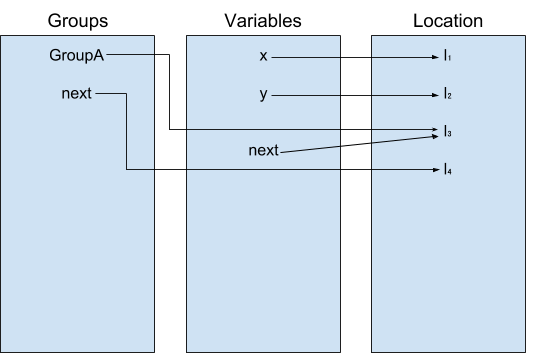
\includegraphics[width=0.7\textwidth]{figures/semantics/5.png}
  \caption{This figure illustrates the next pointer problem}
  \label{fig:ESModelProblem}
\end{figure}
\noindent
As seen on Figure~\ref{fig:ESModelProblem}, the situation where the next pointer in the group environment is updated leaves the next pointer in the variable environment pointing to a location that is already used.
\\\\
To remedy this, we either have to update both next pointers every time either environment is given a new variable, or the next pointer can be moved to storage. The solution employed is the one where the next pointer is moved to storage, as it is the most intuitive.
\\\\
This requires us to redefine the definitions from Subsection~\ref{semantics:EnvStore}. First we redefine the variable environment, as the next pointer has been removed:
\begin{center}
$EnvV = Var \rightharpoonup Loc$
\end{center}
Now the storage is redefined:
\begin{center}
$Sto = Loc \cup \text{\{next\}} \rightharpoonup Number \cup Text \cup Bool \cup Adt \cup Loc $
\end{center}
This states that $Sto$ is a partial function from either a location or the next pointer, that returns either one of the types or a location. The type will be returned if the location is given as input, and likewise the location of the next pointer will be returned when it is given as input.
\subsubsection{Variable declarations}
To declare variables we must define the operational semantics for the \textit{VarDcl} category. 
Variable declarations modify both the storage and the variable environment, due to binding new locations to variables and assigning values to these locations. This gives us the transition relation $\xrightarrow{}\textsubscript{Dv}$ and the system ($\Gamma \textsubscript{Dv}, \xrightarrow{}\textsubscript{Dv}, T \textsubscript{Dv}$). The configurations are defined as:
\\
The possible configurations are $\Gamma \textsubscript{Dv} = (VarDcl \times EnvV \times Sto) \cup EnvV \times Sto$\\
The ending configurations are
$T\textsubscript{Dv} = EnvV \times Sto$ meaning that all variable declarations must point to either a variable or a place in the storage. 
\\\\
As such, the transition takes the shape $\langle D_V, \: env_V, \: sto \rangle \xrightarrow{}\textsubscript{Dv} (env'_v, \: sto')$ In order to construct the semantic rules, we introduce the function $new: Loc \xrightarrow{} Loc$. This function returns the next possible location for any given location. As locations are of the type integer, this is defined as $new l = l + 1$.

\begin{equation}\label{rule:vardcl}
\begin{minipage}{.2\linewidth}
$[\text{AVARDCL}_\text{BSS}]$
\end{minipage}
\begin{minipage}{.8\linewidth}
\centering
$\cfrac{\langle Dv, \: env_v [x \mapsto l], \: sto[l \mapsto v] \: [next \mapsto new \: l]\rangle \xrightarrow{}\textsubscript{Dv} \: (env_v', sto') }{\langle var \: x:= a \: \textit{newline} \: Dv, \: env_v, \: sto \rangle \xrightarrow{}\textsubscript{Dv} \: (env_v', sto')}$
\[where \: env_v, \: sto \vdash a \xrightarrow{}\textsubscript{a} \: v \: and \: l = sto \: \text{next}\]
\end{minipage}
\end{equation}
The rule~\ref{rule:vardcl} shows that we bind $x$ to $l$ where $l$ is the next free location as specified in the side condition. After this, the $next$ pointer is bound to a newly created location after $l$ using the $new$ function.

\subsubsection{Group declarations}
Groups in PHAL are defined in Section~\ref{sec:phalvsarduino}. To relate this to the environment store model, the Figures~\ref{fig:emptyGroup} and \ref{fig:groupA} have been constructed to aid the explanation. 

\begin{figure}[H]
\centering
  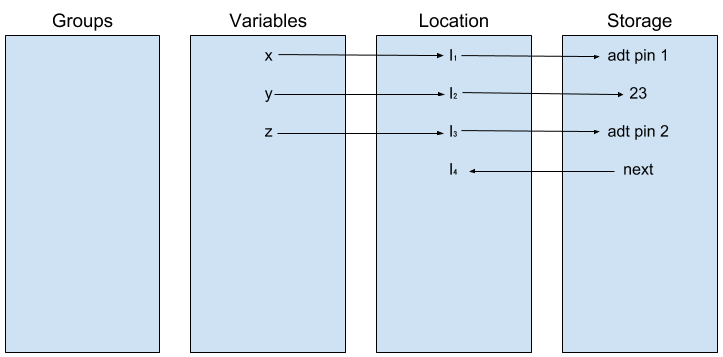
\includegraphics[width=10cm]{figures/semantics/2.png}
  \caption{The expanded model prior to declaration}
  \label{fig:emptyGroup}
\end{figure}
\noindent
Figure~\ref{fig:emptyGroup} shows a visualisation of the environment store model with the added group environment prior to declaring a group. The figure simply illustrates that the functionality of the model is kept intact - variables bind to a location, locations bind to a storage and the next pointer points to the next free location from storage.
\begin{figure}[H]
\centering
  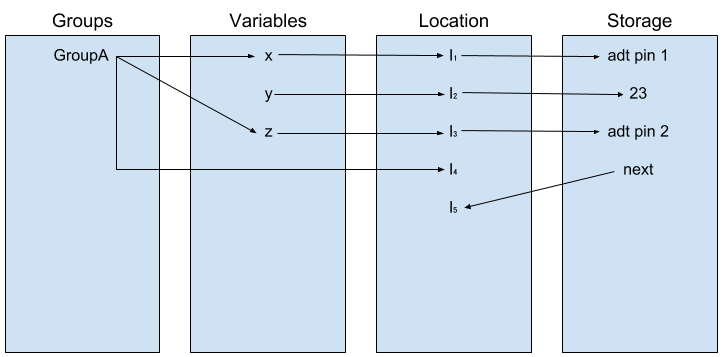
\includegraphics[width=10cm]{figures/semantics/3.png}
  \caption{The expanded model after declaration}
  \label{fig:groupA}
\end{figure}
\noindent
This figure shows the needed functionality for the model when a group has been declared. In order to keep track of the variables contained in the group, we define the \textit{group environment} $EnvG$. This environment is similar to the one defined for variables in Section~\ref{semantics:EnvStore}, but contains bindings from groups to variables rather than variables to location. In order to facilitate a group assignment statement to change the value of all elements of the group, it is also necessary to assign the group to a location during the declaration. Finally, we allow a recursive definition of groups, meaning a group can contain other groups. This gives the following definition:
\\
\begin{center}
$EnvG = GrpNames \rightharpoonup \mathcal{P}(EnvV) \times Loc \times \mathcal{P}(EnvG)$
\end{center}
A single element from $EnvG$ is defined as $env_G$. 
The definition is based on groups only allowing advanced data type variables in their body, as per the definition in Subsection~\ref{Def:Types} and no functions or declarations of any type. The definition  states that for every group name the partial function will return the variables from the variable environment bound to the group. The separate location for the group itself will also be returned, and in the case where a group is an element of another group, the necessary information is returned through the recursive definition of the group environment. This definition is based on the scope rules of PHAL, which states that PHAL uses static scoping for both variables and functions - meaning bindings at the time of declaration needs to be remembered. This is shown in the different through the inclusion of the variable- and group environments. If the scope rules were to be dynamic, the definition would not include these, only returning the location for the group. \cite{PilenVedTraeetsRod}. The location for the group will be put to use in the semantic rules in the statements section, Section~\ref{AppSec:SemanticsStatements}. 
\\\\
Group declarations will modify the storage because the next-pointer needs to be moved to the next free location and it will modify the group environment. The transition system is ($\Gamma \textsubscript{DG}, \xrightarrow{}\textsubscript{DG}, T \textsubscript{DG}$).
\\
The possible configurations are $\Gamma \textsubscript{DG} = (GrpDcl \times EnvG \times Sto) \cup EnvG \times Sto$\\
The ending configurations are
$T\textsubscript{DG} = EnvG \times Sto$\\
This gives transitions the shape: 
\\
\begin{center}
$\langle D_G, env_G, \: sto \rangle \xrightarrow{}\textsubscript{DG} (env'_G, \: sto')$
\end{center}
The rules for declaring groups are seen on \ref{rule:grpdclbss}.
\begin{equation}\label{rule:grpdclbss}
\begin{split}
\begin{minipage}{\linewidth}
$[\text{GRPDCL}_\text{BSS}]$
\end{minipage}
\\
\begin{minipage}{\linewidth}
\centering
$\cfrac{\langle D_G,  \: env_G[gx \mapsto (\{G_B\}, \: l)], \: sto[next \mapsto new \: l] \rangle \xrightarrow{}\textsubscript{DG} (env'_G, sto')}{\langle\text{group} \: gx \: \{G_B\} \: \textit{new} \: D_G, \: env_G, \: sto \rangle \xrightarrow{}\textsubscript{DG}(env'_G, \: sto')}$
\end{minipage}
\\
\begin{minipage}{\linewidth}
\centering
where $env_v, \: sto \vdash \{G_B\} \xrightarrow{}\textsubscript{GB} \: v \text{ and } l = sto \text{ next}$
\end{minipage}
\end{split}
\end{equation}
The side condition states that the content of the body, which is essentially a set of variables, must all be evaluable through the transitions defined for arithmetic expressions, since the rule for evaluating variables, $VAR$, is located in the set defined by the relation for arithmetic expressions. In addition to this, the group receives the next free location prior to updating the next pointer. 
The premise of the rule states that the group-variable \textit{gx} is mapped to the corresponding variables defined in the body of the group, meaning the group can point to multiple variables as defined in the syntactic category $G_B$, and it is also assigned a location through the tuple. Following this. the next pointer in storage is updated to point to a new free location.  


\subsubsection*{List declarations}
Lists in PHAL are used to contain elements of the same type. In order to construct the rules, we introduce a new environment called the list environment $env_L$. This is done for the same reason as the group-environment, the need to keep track of the elements defined in the list. Groups can be an element in a list, given the types are congruent. Lists cannot contain other lists, and a recursive definition is therefore not needed. This functionality is illustrated in Figure~\ref{fig:listgraphic}.

\begin{figure}[H]
\centering
  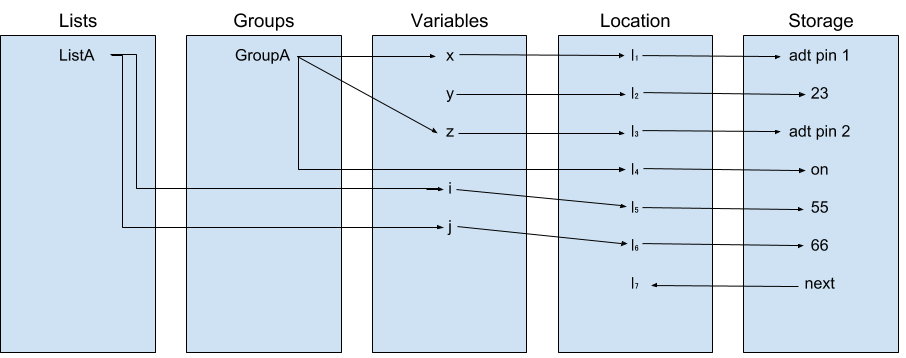
\includegraphics[width=10cm]{figures/semantics/4.png}
  \caption{The model expanded with a list environment}
  \label{fig:listgraphic}
\end{figure}
\noindent
Lists, unlike groups, do not need a location because the list as a whole will not receive a value. A single element in the environment is defined $env_L$. The environment is defined as:
\begin{center}
$EnvL = ListNames \rightharpoonup \mathcal{P}(EnvV) \times \mathcal{P}(EnvG) \times Sto$
\end{center}
Meaning that the list environment is a partial function that maps to the variable environment, group environment or storage the. 
\\\\
Like groups, lists allow all previously declared variables to feature in the declaration. In addition to this, expressions are allowed as elements, meaning the list will point to a value in storage that has to be evaluated through the given expression. This means lists modify the list environment, and the storage in case an expression is present, both through adding the value and moving the next pointer. This gives transitions the shape:
\begin{center}
$\langle D_L,  \: env_L, \: sto\rangle \xrightarrow{}\textsubscript{DL} (env'_L, \: sto')$
\end{center}
The rules for declaration of lists are seen on Rule~\ref{rule:vardcl}.
\begin{equation}\label{rule:listdcl}
\begin{split}
\begin{minipage}{\linewidth}
$[\text{LISTDCL}_\text{BSS}]$
\end{minipage}
\\
\begin{minipage}{\linewidth}
\centering
$\cfrac{\langle D_L,  \: env_L[lx \mapsto \{L_B\}], \: env_L, \: sto \rangle \xrightarrow{}\textsubscript{DL} (env'_L, \: sto')}{\langle\text{list} \: lx \: \{L_B\} \: \textit{new} \: D_L, \: env_L, \: sto \rangle \xrightarrow{}\textsubscript{DL}(env'_L, \: sto')}$
\end{minipage}
\\\\
\begin{minipage}{\linewidth}
\centering
where $env_v, \: sto \vdash \{L_B\} \xrightarrow{}\textsubscript{LB} \: v$
\end{minipage}
\end{split}
\end{equation}
\noindent
The side condition states that all expressions in the body of the list have to be evaluable through the rules established for the body of a list. How the avluation of a constituent \textit{list body} is updated is further elaborated through the rules for the body of the list defined in Appendix~\ref{APP:ListBody}.
\noindent
\subsubsection{Function declarations}
In order to keep track of the necessary information required to execute a function, a procedure environment is introduced. Function declarations update this procedure environment. The transition system is ($\Gamma \textsubscript{Dp}, \xrightarrow{}\textsubscript{Dp}, T \textsubscript{Dp}$), and the configurations are defined as\\
$\Gamma \textsubscript{Dp} = (FuncDcl \times EnvP) \cup EnvP $\\
$T\textsubscript{Dp} = EnvP$
\\
Due to PHAL using static scope rules, transitions take the shape
$env_v, \: env_G, \: env_L \vdash \langle D_P, env_p \rangle \xrightarrow{} \textsubscript{DP} \: env'_P$
\\ 
The other environments are needed to save details about the bindings as part of the information stored about the function \cite{PilenVedTraeetsRod}. Static scope rules mean that only the variable-bindings, group-bindings, list-bindings and procedure-bindings known for a function are those that were in effect when the procedure was declared. Because of this, the procedure-environment needs to remember these bindings, and as such the set $EnvP$ is defined as:
\\\\
$EnvP = Funcnames \rightharpoonup Stmt \times Var \times EnvV \times EnvG \times EnvL \times EnvP $
\\\\
The var component specifies that the formal parameter needs to be remembered.

\begin{equation}\label{rule:funcdclbss}
\begin{split}
\begin{minipage}{\linewidth}
$[\text{FUNCDCL}_\text{BSS}]$
\end{minipage}
\\\\
\begin{minipage}{\linewidth}
\centering
$\cfrac{env_v, \: env_G, \: env_L \vdash \langle D_P, env_p[f \mapsto (S, \: P, \: env_v, \: env_G, \: env_L, \: env_p)]\rangle \xrightarrow{}\textsubscript{DP} \: env'_p}{env_v, \: env_G, \: env_L \vdash \langle \text{define} \: f \: \text{with} \: P \: {F_B} \: \text{returnType} \: RTN \: \textit{newline} D_P, \: env_p\rangle \xrightarrow{}\textsubscript{DP} \: env_p'}$
\end{minipage}
\end{split}
\end{equation}

\noindent
The rule for function declaration can be seen in Rule~\ref{rule:funcdclbss}. In order for function calls to remember the bindings that were in effect during declaration, we explicitly bind the environments to the function $f$ along with the statement to be used and the parameters through $P$. As defined in the syntactic formation in table \ref{tab:syntacticformation}, $P$ can be \textit{none}, one parameter or multiple parameters. The $S$ binding refers to the statements used in the function body $F_B$. 

\subsection*{Function calls}
\begin{equation} \label{EQ:FUNCCALLVALRAP}
\begin{split}
\begin{minipage}{\linewidth}
$[\text{FUNCCALLVAL}_\text{BSS}]$
\end{minipage}
\\\\
\begin{minipage}{\linewidth}
\centering
$\cfrac{env'_v[P \mapsto l_1...l_n] \: env'_G, \: env'_L, \: env'_p \vdash \langle S, sto[l_1...l_n \mapsto v_1...v_n][next \mapsto new \: l], \rangle \xrightarrow{} sto'}{env_v, \: env_G, \: env_L, \: env_p \vdash \langle \text{call} \: f \: \text{with} \: (a_1...a_n), \: sto \rangle \xrightarrow{} sto'}$
\end{minipage}
\\\\
\begin{minipage}{\linewidth}
\centering
where $env_p f = (S, P, env'_v, \: env_G', \: env'_L, \: env'_p),$
\end{minipage}
\\
\begin{minipage}{\linewidth}
\centering
$env_v, \: sto \vdash a_1...a_n \xrightarrow{}\textsubscript{a} \: v_1...v_n$
\end{minipage}
\\
\begin{minipage}{\linewidth}
\centering
$freemem_i = sto[next \mapsto new \: l]$, $l_i = sto \: freemem_i$
\end{minipage}
\\
\begin{minipage}{\linewidth}
\centering
where $1 \leq i \leq n $
\end{minipage}
\end{split}
\end{equation}
\noindent
In call-by-value function calls, the formal parameter appears in the body of the procedure as a local variable. 
This local variable is assigned the value of the actual parameters used for the call. This means that, for each parameter a free memory cell must be found, so that this free memory can contain this local variable, and this variable is initialised with the value of the actual parameter. 
We accomplish this through the side conditions. 
The function is called with $n$ parameters, each one evaluated to a value through the rules for arithmetic expressions. 
After this, the required locations are found through the \textit{free memory (freemem)} variable. 
The store is iterated upon $n$ times, each time finding a new location which is assigned to a location $l$ and the next pointer is updated. 
After this is done, the $n$ found locations are used in the premise of the rule, binding the formal parameters $P$ to their locations. 
As was the case with the FUNCDCL rule (Rule~\ref{rule:funcDcl}), $P$ in this case is either \textit{none}, one parameter or multiple parameters. 
The store is then updated, where the empty locations found are assigned the values evaluated from the actual parameters, creating a correspondence between formal and actual parameters. 
Finally, the next pointer is updated once again, and the store is modified.
\\
\begin{equation} \label{EQ:FUNCCALLRECVALRAP}
\centering
\begin{split}
\begin{minipage}{\linewidth}
$[\text{FUNCCALLRECVAL}_\text{BSS}]$
\end{minipage}
\\
\begin{minipage}{\linewidth}
\centering
$
\dfrac
    {
    \splitdfrac
        {
            env'_v[P \mapsto l_1...l_n], \: env'_G, \: env'_L, \: env'_p[f \mapsto (S, \: P, \: env'_v, \: env'_G, \: env'_L \: env'_p)]
        }
        { 
            \vdash \langle S, sto[l \mapsto v][next \mapsto new \: l] \rangle \xrightarrow{} sto'
        }
    }
    {
        env_v, \: env_G, \: env_L, \: env_p \vdash \langle \text{call} \: f \: \text{with} \: (a_1...a_n), \: sto \rangle \xrightarrow{} sto'
    }
$
\end{minipage}
\\\\
\begin{minipage}{\linewidth}
\centering
where $env_p f = (S, P, env'_v, \: env_G', \: env'_L, \: env'_p),$
\end{minipage}
\\
\begin{minipage}{\linewidth}
\centering
$env_v, \: sto \vdash a_1...a_n \xrightarrow{}\textsubscript{a} \: v_1...v_n$
\end{minipage}
\\
\begin{minipage}{\linewidth}
\centering
$freemem_i = sto[next \mapsto new \: l]$, $l_i = sto \: freemem_i$
\end{minipage}
\\
\begin{minipage}{\linewidth}
\centering
where $1 \leq i \leq n $
\end{minipage}
\end{split}
\end{equation}
\\
This rule is very similar to \ref{EQ:FUNCCALLVALRAP}, but the main difference is found in the procedure-environment used in the premise of the rule. In the previous rule for function calls, $S$ is executed in the procedure-environment $env'_p$, which includes the procedure-bindings known before $f$ was declared. This means that, if we were to execute a second call of $f$ in the statement $s$, the second call in the body would be a different procedure compared to the first call, because $f$ is not declared in $env'_p$ and as such $f$ is not known in that environment. To allow recursive calls, the procedure-environment must then contain a binding of the original function, where the information needed to execute the original function is stored, and the statement $S$ must be executed in the procedure environment that is updated with the binding of $f$. This means we first look up the bindings at the time of declaration, and then create a new environment where these bindings are kept so they can be called recursively.


\subsection*{Statements}
\begin{equation}\label{rule:assignabss}
\begin{minipage}{.2\linewidth}
$[\text{ASSIGNA}_\text{BSS}]$
\end{minipage}
\begin{minipage}{.8\linewidth}
\centering
$env_v \vdash \langle x := a, \: sto \rangle \xrightarrow{} sto[l \mapsto v]$
\\
where $env_v, \: sto \vdash a \xrightarrow{}\textsubscript{a} \: v$ and $env_v \: x = l$
\end{minipage}
\end{equation}
In Rule~\ref{rule:assignabss} the simplest form for statement is seen. It handles binding a variable to an arithmetic expression, \textit{a}. The side condition states that \textit{a} must be evaluated to a value and \textit{x} is a location in the variable environment. Finally the value is mapped to the location in the storage \textit{sto}.


\begin{equation}\label{rule:loopuntiltrue}
\begin{minipage}{.2\linewidth}
$[\text{LOOPUNTIL-TRUE}_\text{BSS}]$
\end{minipage}
\begin{minipage}{.8\linewidth}
\centering
$env_v, \: env_p \vdash \langle $loop $S$ until $b$, sto$\rangle \xrightarrow{} sto$ \\
if $env_v, \: sto \vdash b \xrightarrow{}\textsubscript{b} \: tt$ 
\end{minipage}
\end{equation}
In Rule~\ref{rule:loopuntiltrue}, the boolean expression \textit{b} is evaluated immediately before any iterations of the loop, and as such, if the expression evaluates to true no iteration is conducted. This is evident in the side-condition, where $b$ is evaluated in the original \textit{sto}, rather than the updated store \textit{sto'} which would be created if $b$ were to be evaluated after the iteration of the loop.

\begin{equation}
\begin{split}
\begin{minipage}{\linewidth}
$[\text{LOOPUNTIL-FALSE}_\text{BSS}]$
\end{minipage}
\\\\
\begin{minipage}{\linewidth}
\centering
$\cfrac{env_v \: env_p \vdash \langle S, \: sto \rangle \xrightarrow{} sto'' \quad\: env_v, \: env_p \vdash \langle \text{loop} \: S \: \text{until} \: b, \: sto'' \rangle \xrightarrow{} sto'}{env_v, \: env_p \vdash \langle \text{loop} \: S \: \text{until} \: b, \: sto \rangle \xrightarrow{} sto'}$ 
\end{minipage}
\\\\
\begin{minipage}{\linewidth}
\centering
if $env_v, \: sto \vdash b \xrightarrow{}\textsubscript{b} \: ff$
\end{minipage}
\end{split}
\end{equation}
In order to define the statement that loops S a certain amount of times, we introduce a function that, for any given number, gives the corresponding numeral, the inverse of the function introduced for the arithmetic expressions:
\begin{center}
$\mathcal{N}^{-1}: \mathbb{Z} \xrightarrow{} Num$
\end{center}
This function uses the set of integers, denoted $\mathbb{Z}$, as the number cannot be a floating point number.
\begin{equation}\label{rule:looptimesbss}
\begin{split}
\begin{minipage}{\linewidth}
$[\text{LOOPTIMES}_\text{BSS}]$
\end{minipage}
\\
\begin{minipage}{\linewidth}
\centering
$\cfrac{env_v, \: env_p \vdash \langle S, \: sto \rangle \xrightarrow{} sto'' \: \: \: \: \: \langle \text{loop} \: S \: n \: \text{times}, \: sto'' \rangle \xrightarrow{} sto'}{env_v, \: env_p \vdash \langle \text{loop} \: S \: a \: \text{times} \rangle \xrightarrow{} sto'}$ 
\end{minipage}
\\\\
\begin{minipage}{\linewidth}
\centering
where $env_v, \: sto \vdash a \xrightarrow{} v$
\\
$n = \mathcal{N}^{-1}(v-1)$
\\
$v > 0$
\end{minipage}
\end{split}
\end{equation}
\noindent
The rule~\ref{rule:looptimesbss} states that the loop condition is tested at first in state $s$. This creates a new state $s''$, which is then used for the execution of the actual loop body, finally ending with state $s'$ in both the premise and the conclusion of the rule. The side conditions details when the loop condition is met. The first condition states that the arithmetic expression in state $s$ must be evaluable to a value. The second condition makes use of the function defined above to give the corresponding numeral for the given number based on $v$, where $v$ is decremented for each iteration of the loop. Finally the last condition ensures that the loop is only executed when the value of the arithmetic expression is a positive numeral, this can be seen on rule~\ref{rule:looptimesend}.
\begin{equation}\label{rule:looptimesend}
\begin{minipage}{.2\linewidth}
$[\text{LOOPTIMES-END}_\text{BSS}]$
\end{minipage}
\begin{minipage}{.8\linewidth}
\centering
$env_v, \: env_p \langle \text{loop} \: S \: a \: \text{times}, \: sto \rangle \xrightarrow{} sto$ 
\\
where $env_v, sto \vdash a \xrightarrow{} v \: \text{and} \: v \leq 0$
\end{minipage}
\end{equation}

\subsection*{Switch}
\begin{equation}\label{rule:switchdefault}
\begin{split}
\begin{minipage}{\linewidth}
$[\text{SWITCH-DEFAULT}_\text{BSS}]$
\end{minipage}
\\
\begin{minipage}{\linewidth}
\centering
$\cfrac{env_v, \: env_p \vdash \langle S, \: sto \rangle \xrightarrow{} sto'}{env_v, \: env_p \vdash \langle \text{switch}(e) \{\text{case} <e_1>: \: S_1  \: \text{default:} \: S\}, \: sto \rangle \xrightarrow{} sto' }$ 
\end{minipage}
\\\\
\begin{minipage}{\linewidth}
\centering
where $env_v, \: env_p \vdash e \xrightarrow{} v$
\\
$env_v, \: env_p \vdash e_1 \xrightarrow{} v_1$
\\
$v \neq v_1$
\end{minipage}
\end{split}
\end{equation}
Rule \ref{rule:switchdefault} defines the case where $n=1$, meaning there is only one switch case followed by the default case. In this case, if the expression being switched can evaluate to a value, and the expression of the first case can evaluate to a value, but these values are not similar, the switch will execute the default statement $S$ in state $s$.
\begin{equation}\label{rule:switch1bss}
\begin{split}
\begin{minipage}{\linewidth}
$[\text{SWITCH-1}_\text{BSS}]$
\end{minipage}
\\
\begin{minipage}{\linewidth}
\centering
$\cfrac
{
    env_v, \: env_p \vdash \langle S_1, \: sto \rangle \xrightarrow{} sto'
}
{
   env_v, \: env_p \vdash \langle \text{switch}(e) \{\text{case} <e_1>: \: S_1 ... \text{case} <e_n>: \: S_n \: \text{default:} \: S\}, \: sto \rangle \xrightarrow{} sto' 
}
$ 
\end{minipage}
\\\\
\begin{minipage}{\linewidth}
\centering
if $ n \geq 1$ and $env_v, \: env_p \vdash e \xrightarrow{} v$
\\
$env_v, \: env_p \vdash e_1 \xrightarrow{} v_1$
\\
$v = v_1$
\end{minipage}
\end{split}
\end{equation}
The Rule~\ref{rule:switch1bss} accounts for the possibility where $n$ is greater than or equal to $1$, meaning it is possible to have multiple cases not including the default case, but the value of $e$ is evaluated to the value of $e_1$, making the first case the one to be executed. In the case where $ n = 1$, meaning there is only one case and the default, this rule serves as the opposite of the SWITCH-DEFAULT rule, executing the first case.
\begin{equation}\label{rule:switch2bss}
\begin{split}
\begin{minipage}{\linewidth}
$[\text{SWITCH-2}_\text{BSS}]$
\end{minipage}
\\
\begin{minipage}{\linewidth}
\centering
$\cfrac
{
    env_v, \: env_p \vdash \langle  \text{switch}(e) \{\text{case} <e_2>: \: S_2 ... \text{case} <e_n>: \: S_n \: \text{default:} \: S\}, \: sto \rangle \xrightarrow{} sto'
}
{
    env_v, \: env_p \vdash \langle \text{switch}(e) \{\text{case} <e_1>: \: S_1 ... \text{case} <e_n>: \: S_n \: \text{default:} \: S\}, \: sto \rangle \xrightarrow{} sto' 
}$ 
\end{minipage}
\\\\
\begin{minipage}{\linewidth}
\centering
if $ n > 1$ and $env_v, \: env_p \vdash e \xrightarrow{} v$
\\
$env_v, \: env_p \vdash e_1 \xrightarrow{} v_1$
\\
$v \neq v_1$
\end{minipage}
\end{split}
\end{equation}
The Rule~\ref{rule:switch2bss} deals with the possibility of having multiple cases, meaning that $n$ is strictly greater than 1, and the first case not matching the value evaluated. In this case, the premise removes the first option that was evaluated to false, and the next expression in line is evaluated according to $e$. This rule interacts with SWITCH-1 (Rule~\ref{rule:switch1bss}), as they in unison serve to find the correct case. If $n$ reaches $1$, and this is once again evaluated to be different than the original expression, the SWITCH-DEFAULT rule (Rule~\ref{rule:switchdefault}) ensures that the switch is terminated properly.

\subsubsection{If-else}

\begin{equation}\label{sem:IfNoElseTT}
\begin{minipage}{.2\linewidth}
$[\text{IFNOELSE-TRUE}_\text{BSS}]$
\end{minipage}
\begin{minipage}{.8\linewidth}
\centering
$\cfrac{env_v, \: env_p \vdash \langle S, \: sto\rangle \xrightarrow{} sto'}{env_v, \: env_p \vdash \langle \text{if} \: b \: \text{then} \: S, \: sto \rangle \xrightarrow{} sto'}$ 
\\
if $env_v, \: sto \vdash b \xrightarrow{}\textsubscript{b} \: tt$
\end{minipage}
\end{equation}
The Rule~\ref{sem:IfNoElseTT} deals with the simplest case of an if-statement, where there is no following else statement. In this case, if the expression is evaluated to true, the statement $S$ is executed and the storage is updated.\\
In the opposite case, where the expression evaluates to false, there will be no further consequences of the rule. The rule for this can be found on Rule~\ref{listing:ifnoelse-false}.
\\
If-statements can chain together multiple \textit{else-if} clauses. In order to facilitate this, the syntactic category $S_{if}$ is introduced. In this category, three possibilities for ending if-statements are detailed. The two following rules deal with the if-statements found in the S category that contain the $S_{if}$ category.
\begin{equation}\label{rule:ifelsetrue}
\begin{minipage}{.2\linewidth}
$[\text{IFELSE-TRUE}_\text{BSS}]$
\end{minipage}
\begin{minipage}{.8\linewidth}
\centering
$\cfrac{env_v, \: env_p \vdash \langle S, \: sto \rangle \xrightarrow{} sto'}{env_v, \: env_p \vdash \langle \text{if} \: b \: \text{then} \: S \:S_{if}, \: sto \rangle \xrightarrow{} sto'}$ 
\\
if $env_v, \: sto \vdash b \xrightarrow{}\textsubscript{b} \: tt$
\end{minipage}
\end{equation}
The Rule~\ref{rule:ifelsetrue} is similar to the one detailing if-structures without else clauses seen in Rule~\ref{sem:IfNoElseTT}. The only difference is in the conclusion, in the way the if-structure is detailed. For this rule, the use of an else clause is allowed, but specifies that the condition for the \textit{if} is evaluated to true, and as such, the statement $S$ related to the \textit{if} is executed.
\\\\
The case where the boolean expression $b$ evaluates to false requires the use of the $s_{if}$ category, and the rules for this category will be detailed in the following section.
\textbf{The $S_{if}$ category}\\
The Rules~\ref{rule:elseifseqtrue} and \ref{rule:elseifseqtrue} detail the possible endings to if-statements in PHAL.

\begin{equation}\label{rule:elseifseqtrue}
\begin{minipage}{.2\linewidth}
$[\text{ELSEIFSEQ-TRUE}_\text{BSS}]$
\end{minipage}
\begin{minipage}{.8\linewidth}
\centering
$\cfrac{env_v, \: env_p \vdash \langle S, \: sto \rangle \xrightarrow{} sto'}{env_v, \: env_p \vdash \langle \text{else if} \: b \: \text{then} \: S \: S_{if}, \: sto \rangle \xrightarrow{} sto'}$ 
\\
if $env_v, \: sto \vdash b \xrightarrow{}\textsubscript{b} \: tt$
\end{minipage}
\end{equation}
This rule describes the case where there's an \textit{else-if} statement following an \textit{if}, and the \textit{else-if} evaluates to true.\\
In this case, the statement $S$ bound to the \textit{else-if} clause is executed and the storage is updated.

\begin{equation}\label{rule:elseend}
\begin{minipage}{.2\linewidth}
$[\text{ELSEEND}_\text{BSS}]$
\end{minipage}
\begin{minipage}{.8\linewidth}
\centering
$\cfrac{env_v, \: env_p \vdash \langle S, \: sto \rangle \xrightarrow{} sto'}{env_v, \: env_p \vdash \langle \text{else} \: S, \: sto \rangle \xrightarrow{} sto'}$ 
\end{minipage}
\end{equation}
Rule~\ref{rule:elseend} defines the case where an \textit{else} clause is defined in the \textit{if}-structure, and all the previous cases evaluated to false. In this case, this means that the statement $S$ bound to the \textit{else}-clause is executed by default, updating the storage.

\section{Type rules}\label{subsec:FormalTypeRules}
In order to precisely define the type rules we create a type system for PHAL. The type system is used to define a classification for the syntactic entities of a program. This is used as a guarantee to prevent the runtime errors that the type system aims to prevent.  A simple example of why type system are useful can be found in the following expression that is allowed in PHAL:
\begin{center}
$12 + (12 > 14)$
\end{center}
This expression attempts to add a boolean expression and a numeral that evaluates to the PHAL type \textit{number}. This would lead to a runtime error. This can be avoided by giving both components of the expression a type, and requiring in an addition expression that both components need to be of the type \textit{number} to avoid errors. For PHAL, the types used in the type system are the same as the ones defined in Section~\ref{Def:Types} - \textit{bool, number, text, group and list}. A type system consists of:
\begin{itemize}
    \item A definition of the set of types
    \item A definition of the type judgement for the elements of each syntactic category in the language
    \item A number of type rules for each category that define the valid type judgement\cite{PilenVedTraeetsRod}
\end{itemize}

\subsubsection{Operator precedence-table}
In addition to the type rules, the precedence and associativity of the operators must be specified. The precedence of operators ensures that the operator grammar is unambiguous. 
It was chosen to use a precedence that imitates the operator precedence that is used in mathematics. This is done to ensure that the arithmetic operations and logical operations in PHAL are as intuitive as possible for the user. 

\begin{table}[H]
\centering
\caption{Operator precedence for PHAL}
\label{tab:operatorprecedence}
\begin{tabular}{|l|l|l|l|}
\hline
\textbf{Precedence} & \textbf{Operator}                                                                                                                                                                       & \textbf{Description}                                                                                                                                                                             & \textbf{Associativity} \\ \hline
1                   & ( )                                                                                                                                                                                     & Subexpression                                                                                                                                                                                    & Left to right          \\ \hline
2                   & \begin{tabular}[c]{@{}l@{}}!\\ not\end{tabular}                                                                                                                                         & \begin{tabular}[c]{@{}l@{}}Logical negation\\ Logical negation\end{tabular}                                                                                                                      & Left to right          \\ \hline
3                   & \begin{tabular}[c]{@{}l@{}}*\\ /\end{tabular}                                                                                                                                           & \begin{tabular}[c]{@{}l@{}}Multiplication\\ Division\end{tabular}                                                                                                                                & Left to right          \\ \hline
4                   & \begin{tabular}[c]{@{}l@{}}+\\ -\end{tabular}                                                                                                                                           & \begin{tabular}[c]{@{}l@{}}Plus or concatenation\\ Minus\end{tabular}                                                                                                                            & Right to left          \\ \hline
5                   & \begin{tabular}[c]{@{}l@{}}\textless\\ is less than\\ \textless=\\ is less than or equal to\\ \textgreater\\ is greater than\\ \textgreater=\\ is greater than or equal to\end{tabular} & \begin{tabular}[c]{@{}l@{}}Less than\\ Less han\\ Less than or equal to\\ Less than or equal to\\ Greater than\\ Greater than\\ Greater than or equal to\\ Greater than or equal to\end{tabular} & Left to right          \\ \hline
6                   & \begin{tabular}[c]{@{}l@{}}=\\ is\\ !=\\ is not\end{tabular}                                                                                                                            & \begin{tabular}[c]{@{}l@{}}Equality comparison\\ Equality comparison\\ Inequality comparison\\ Inequality comparison\end{tabular}                                                                & Left to right          \\ \hline
7                   & \begin{tabular}[c]{@{}l@{}}\&\\ and\end{tabular}                                                                                                                                        & \begin{tabular}[c]{@{}l@{}}Logical and\\ Logical and\end{tabular}                                                                                                                                & Left to right          \\ \hline
8                   & \begin{tabular}[c]{@{}l@{}}or\\ ||\end{tabular}                                                                                                                                         & \begin{tabular}[c]{@{}l@{}}Logical or\\ Logical or\end{tabular}                                                                                                                                  & Left to right          \\ \hline
9                   & :=                                                                                                                                                                                      & Assignment                                                                                                                                                                                       & Right to left          \\ \hline
\end{tabular}
\end{table}

\noindent
\subsubsection*{Changes to the abstract syntax}
When creating the rules for the semantics of PHAL, we defined an abstract syntax as shown in Table~\ref{tab:syntacticcategories}, Section~\ref{Def:Semantics}. To create the type system, this syntax is modified to include type for declarations of the different categories of variables. To do this, we use the metavariable $T$ to define an element of the category of types defined as \textit{Types}. 
\begin{table}[H]
\centering
\begin{tabular}{@{}lll@{}}
\toprule
Variable &       & Description                      \\ \midrule
$e$       & $::=$ &  $n$ | $x$ | $gx$ | $lx$ | $e_1 + e_2$ | $e_1 - e_2$ | $e_1 * e_2$ | $e_1 \div e_2$ | $e_1 \bmod e_2$ | $ (e_1)  $ \\
          && | $e_1 = e_2$ | $e_1 != e_2$ | $e_1 > e_2$ | $e_1 >= e_2$            \\
            & & | $!e$ | $e_1$ \& $e_2$ | $e_1 | e_2$ \\
            &&  | $e_1$ is $e_2$ | $e_1$ and $e_2$  | $e_1$ or $e_2$ |  $e_1$ is not $e_2$ | not $e$ \\
            &&  | $e_1$ greater than $e_2$  |  $e_1$ less than $e_2$  | $e_1$ less than or equal to $e_2$ \\
            &&  | $e_1$ greater than or equal to $e_2$ \\
            & & | true | false | on | off \\
$S$        & $::=$ & $x:= e$ | $gx := e$ | $S_1 \textit{new} \: S_2$ | if ($e$) then \{$S$\} $S_{if}$ | if ($e$) then \{$S$\} \\
           & & | loop $S$ until $e$ | loop $S$ until $e$, increase x by n    \\
           & & | loop $S$ until $e$, decrease $x$ by $n$ | loop $S$ $e$ times \\
           & & | call $f$ with ($e...e_n$)  \\
           & & | switch($e$) \{case $<e_1>: \: S_1$ $...$ case $<e_n>: \: S_n$ default: $S$ \} \\
           &&  | get element $n$ from $lx$ | remove element $n$ from $lx$  \\
           &&  | add $e$ to $lx$ |  $\text{wait for } e \text{ seconds}$  \\
$S_{if}$     & $::=$ &  else if ($e$) then \{$S$\} | else if ($e$) then \{$S$\} $S_{if}$ |  else \{$S$\} \\
$D_V$       & $::=$ & $T \: var$ $x := e \: \textit{new}$ $D_V$ | $\epsilon$ \\
$D_G$       & $::=$ & $T \: var \: gx\{ G_B \} \: \textit{new} \: D_G | \: \epsilon$ \\
$D_L$     & $::=$ &  $T \: var \: lx\{ L_B \} \: \textit{new} \: D_L | \: \epsilon$ \\
$D_F$       & $::=$ & define $f$ with ($T \: P$) \{$F_B\} \: \text{returnType} \: (RTN) \: \textit{new}$ $D_F$ | $\epsilon$ \\
$D_P$  & $::=$ &  $T \: x, \: D_P \: | \: T \: x $  \\
$D_{Adt}$   & $::=$ & $T \: var$ $x$ $:=$ pin $Pin \: new \: D_{adt} | \: \epsilon  $\\
\bottomrule
\end{tabular}
\caption{Syntactic formation of PHAL updated for the type system}
\label{tab:syntacticformationtypes}
\end{table}
\noindent
Table~\ref{tab:syntacticformationtypes} has removed the metavariables $a$ and $b$ used for defining the semantics of PHAL, and swapped all occurrences of these with the metavariable $e$, to denote a generalised expressions. This also means that the occurrences of $a$ or $b$ in the statement elements have been swapped to $e$. Because of this change, we update the previous table of syntactic categories shown on Table~\ref{tab:syntacticcategories}to reflect the introduction of $e$:
\begin{table}[H]
\centering
\begin{tabular}{@{}lll@{}}
\toprule
Variable &       & Description                      \\ \midrule
$n$        & $\in$ & \textbf{Num} - Number                     \\
$x$        & $\in$ & \textbf{Var} - Variable                     \\
$gx$        & $\in$ & \textbf{GVar} - A variable of the group type                     \\
$lx$        & $\in$ & \textbf{LVar} - A variable of the list type                     \\
$\epsilon$ & $\in$ & \textbf{Epsilon} - The empty string \\
$new$      & $\in$ &  \textbf{Newl} - Newline                   \\
$e$        & $\in$ & \textbf{Exp} - The combined category for arithmetic and boolean expressions                \\
$adt$        & $\in$ & \textbf{Adv} - Advanced data type                     \\
$f$       & $\in$ & \textbf{FuncName} - The name of a function      \\
$S$        & $\in$ & \textbf{Stmt} - Statements               \\
$D_V$       & $\in$ & \textbf{VarDcl} - Declaration of a variable \\
$D_G$       & $\in$ & \textbf{GroupDcl} - Declaration of a group \\
$D_L$       & $\in$ & \textbf{ListDcl} - Declaration of a list \\
$D_F$       & $\in$ & \textbf{FuncDcl} - Declaration of a function \\
$D_{Adt}$       & $\in$ & \textbf{AdvDcl} - Declaration of an advanced type      \\
$D_P$       & $\in$ & \textbf{ParamDcl} - Declaration of parameters for a function \\
$P$       & $\in$ & \textbf{ParamOpt} - The parameter options \\
$Pin$      & $\in$ &  \textbf{Pins} - The pins that are used to connect the Arduino \\
$RTN$       & $\in$ & \textbf{Rtrn} - The returntypes \\
$P_S$        & $\in$ & \textbf{ProgStart} - The start of the program \\
$S_B$       & $\in$ & \textbf{SetBody} - The construction of setup      \\
$G_B$       & $\in$ & \textbf{GrpBody} - The body of the group \\
$L_B$       & $\in$ & \textbf{ListBody} - The body of the list \\
$L_T$       & $\in$ & \textbf{ListType} - The type of the list \\
$F_B$      & $\in$ &  \textbf{FuncBody} - The user defined function body  \\ 
$F_N$      & $\in$ &  \textbf{FuncNames} - The function names  \\
$L_N$      & $\in$ &  \textbf{ListNames} - The list names  \\
$G_N$      & $\in$ &  \textbf{GrpNames} - The group names  \\\bottomrule
\end{tabular}
\caption{Syntactic categories of PHAL}
\label{tab:updatedsyntacticcategories}
\end{table}
\noindent 
We can now define a new transition system for expressions that includes both of the previous definitions:

\begin{equation*}
(\textbf{Exp} \cup \; \mathbb{Q} \cup \; \{tt, \; ff\}, \: \xrightarrow{}\textsubscript{e}, \: \mathbb{Q} \cup \; \{tt, \; ff\})    
\end{equation*}
The transition relation $\xrightarrow{}\textsubscript{e}$ is defined by the updated list of rules given for expressions in Appendix~\ref{typerules:TypeRules}, Section~\ref{typerules:UpdatedExpressions}.

\subsubsection{The types in the type system}
The type system contains the following types:
\begin{equation}
\begin{split}
\text{B} &::= \text{number } | \text{ text } | \text{ bool } | \text{ group } | \text{ list } | \text{ motor } | \text{ temperatureSensor } | \text{ lightbulb}
\\
\text{G} &::= \text{ motor } | \text{ temperatureSensor } | \text{ lightbulb}
\\
\text{T} &::= \text{B } | \text{ G } |  \: x_1...x_n  : B_1...B_n \xrightarrow{} \text{ok } | \text{ ok}
\end{split}
\label{typerules:basistypes}
\end{equation}
The category of types is named $Types$, and elements of this category are denoted with the metavarabile $T$. The concrete types of PHAL are represented as a subset of all types T, denoted by the metavariable $B$ for basic types. Because groups are limited in which types they can contain, a category for the valid group types is also defined as a subset of $T$, denoted $G$.
The type of a function will be the composite type $x_1...x_n : B_1...B_n \xrightarrow{} \text{ok}$, which states that if the types of the formal parameters of the function are $B$, then the statement executing the functions body will be well-typed \cite{PilenVedTraeetsRod}. We also add the type \textit{ok}, which is the type of statements, declarations and functions if they do not have any type errors. These types are shown as part of the category for all types $T$ on Equation~\ref{typerules:basistypes}. 



\subsubsection{Type environments}
To keep track of the type of any given variable we introduce a type environment. This type environment is defined as the partial function:
\begin{align}\label{TypeRules:EDefinition}
    \text{E} : \text{Var} \cup \text{FuncNames} \rightharpoonup \text{Types}
\end{align}
We also need to be able to update type-environments. We let $E$ be a type environment, and let $E[x \mapsto T]$ describe the type environment $E'$ defined by:
\\\\
\begin{equation*}
    E'(y)=
    \begin{cases}
    E(y) \;\; &\text{if} \; y \neq x\\
    T \;\;    &\text{if} \; y = x
    \end{cases}
\end{equation*}
\\\\
This definition states that we want to update the environment $E$ by mapping the variable $x$ to the type $T$ in the environment. We do this by looking through the current environment $E$ searching for the variable we want to update, denoted by $y$. This is written as $E(y)$. If we find a variable $x$ matching the $y$ variable, we know that the correct variable exists in the environment, and we update it with type $T$, resulting in the updated environment $E'(y)$. If no matching variable is found, it does not exists in the environment an error occurred and no change can be made.
\\\\
\textbf{The format of type judgements}
\\\\
The \textit{type judgements} tell us the  following, where the environment $E$ is defined as in Equation~\ref{TypeRules:EDefinition}:
\\\\
$E \vdash e : T$ - an expression has a type $T$
\\\\
$E \vdash D_v : \text{ok}$ - variable declarations have the type \textit{ok}
\\\\
$E \vdash D_f : \text{ok}$ - function declarations have the type \textit{ok}
\\\\
$E \vdash D_G : \text{ok}$ - group declarations have the type \textit{ok}
\\\\
$E \vdash D_L : \text{ok}$ - list declarations have the type \textit{ok}
\\\\
$E \vdash S : \text{ok}$ - statements declarations have the type \textit{ok}
\\\\
$E \vdash S_{if} : \text{ok}$ - if-statement-ending have the type \textit{ok}
\\\\
$E \vdash Pin : Number$ - pins are required to be of the type \textit{number}
\\\\
Because these different categories can include variables, the type-environment $E$ is included as a prerequisite for the type judgements. In the following section we will describe the rules that detail how you assign types to the syntactic elements for some chosen categories. The remaining rules can be found in Appendix~\ref{app:typerulesforvalid}.
\\\\
\textbf{Type rules for valid type judgements for expressions}
\begin{equation}\label{eq:addnum}
\begin{minipage}{.2\linewidth}
$[\text{ADDNUM}_\text{EXP}]$ 
\end{minipage}
\begin{minipage}{.8\linewidth}
\centering
$\cfrac{E \vdash e_1 : \text{Number } \: \: E \vdash e_2 : \text{Number}}{E \vdash e_1 + e_2 : \text{Number}}$
\end{minipage}
\end{equation}
\begin{equation}\label{eq:addtext}
\begin{minipage}{.2\linewidth}
$[\text{ADDTEXT}_\text{EXP}]$ 
\end{minipage}
\begin{minipage}{.8\linewidth}
\centering
$\cfrac{E \vdash e_1 : \text{Text } \: \: E \vdash e_2 : \text{Text}}{E \vdash e_1 \circ e_2 : \text{Text}}$
\end{minipage}
\end{equation}
\noindent
The \textit{add} rule has been split into two, to accommodate the operator overloading. In Listing~\ref{eq:addnum} the rule for adding two numbers is seen. 
It requires the expressions $e_1$ and $e_2$ to both evaluate to a \textit{Number}, in this case the numeric value of the two can be added together using the mathematical addition rule.
\\\\
Likewise, if $e_1$ and $e_2$ are of type \textit{Text}, the rule for adding two \textit{Text} types can be used. 
This rule can be seen on Listing~\ref{eq:addtext}. 
The main difference being that instead of using the mathematical addition rule, they are concatenated. 




\begin{equation}
\begin{minipage}{.2\linewidth}
$[\text{VAR}_\text{EXP}]$
\end{minipage}
\begin{minipage}{.8\linewidth}
\centering
$\cfrac{E(x) = T} {E \vdash x : T}$
\end{minipage}
\end{equation}
This rule simply states that we look for $x$ in the environment $E$ through the $E(x)$ notation, and this returns the type of $x$.

\begin{equation}\label{TypeRules:GrpVar}
\begin{minipage}{.2\linewidth}
$[\text{GRPVAR}_\text{EXP}]$
\end{minipage}
\begin{minipage}{.8\linewidth}
\centering
$\cfrac{E[gx \mapsto (x_1...x_n : G_1...G_n)] \vdash E(gx) = \text{ok} } {E \vdash gx : \text{ok}}$
\end{minipage}
\end{equation}
Groups can only contain a certain set of types, therefore it is needed to check if each element can be evaluated to type $G$, meaning that they are correctly defined. If this is the case, the type of the group variable when looked up in environment $E$ will be $ok$, as groups in PHAL do not have a specific type by themselves, but ensure a combination of different types can be used by the programmer.


\begin{equation}
\begin{minipage}{.2\linewidth}
$[\text{LISTVAR}_\text{EXP}]$
\end{minipage}
\begin{minipage}{.8\linewidth}
\centering
$\cfrac{E[lx \mapsto (gx_1...gx_n : ok,\: x_1...x_n : T \xrightarrow{} ok)] \vdash E(lx) = T } {E \vdash lx : T}$
\end{minipage}
\end{equation}
Lists can contain groups and variables. This means the environment $E$ has to be updated with the bindings of the components of the list. If the group variables can be evaluated to type $ok$, it means that the constituent variables of each group are correctly typed as defined in the rule for type checking groups, Rule~\ref{TypeRules:GrpVar}. On top of this, the bindings for the separate variables in the list must be correctly typed as type $T$. If the conditions are met, the list variable $lx$ can be looked up in the environment and typed as $T$. 

\subsubsection{Type rules for declarations}
To construct the type rules for declarations we need to define certain helper functions. These functions need to return the updated type-environment given by a declaration, when we know the type-bindings for the environment $E$ prior to the declaration. The functions are defined as such:
\begin{equation}\label{typehelp1}
    E(\epsilon, \: E) = E
\end{equation}

\begin{equation}\label{typehelp2}
    E(T \: var \: x := e \: new \: D_V, \: E) = E(D_V, \: E[x \mapsto T])
\end{equation}

\begin{equation}\label{typehelpADT}
    E(T \: var \: x := \text{pin} \: Pin \: new \: D_{adt}, \: E) = E(D_{adt}, \: E[x \mapsto T])
\end{equation}

\begin{equation}\label{typehelp3}
    E(T \: var \: gx := \{G_B\} \: new \: D_G, \: E) = E(D_G, \: E[gx \mapsto (x_1...x_n : T_1...T_n)\xrightarrow{}ok])
\end{equation}

\begin{equation}\label{typehelp4}
    E(T \ var \ lx \: := \: \{L_B\} \: new \: D_L, \: E) = E(D_L, \: E[lx \mapsto (gx_1...gx_n : T_1...T_n \xrightarrow{} ok, \: x_1...x_n : T_1...T_n \xrightarrow{} ok)])
\end{equation}

 \begin{equation} \label{typehelp5}
     E(\text{define} \, f \, \text{with} \, (T \, P) \, \{F_B\} \, \text{returnType} \, (RTN) \, new \, D_F, \, E) = E(D_F, \, E[f \mapsto (P:T_1...T_n) \xrightarrow{}\text{ok}])
 \end{equation}
\\
These functions define the resulting type environment after declarations. In the case of function \ref{typehelp1}, it states that updating type-environment $E$ with $\epsilon$ is equivalent to an environment that is unchanged as it is an empty declaration. Function \ref{typehelp2} concerns declarations of variables. It states that when the environment $E$ is updated with a variable declaration, the updated type-environment is one where the variable $x$ defined in the declaration is mapped to the type $T$. The next function, Function~\ref{typehelpADT} is similar to Function~\ref{typehelp2}.
\\\\
Function \ref{typehelp3} describes the updated environment after a group has been declared. The environment $E$ is updated to contain a variable $gx$, of type ok if all of the $n$ elements contained in the group can evaluate to a type $T$. The next function, Function~\ref{typehelp4}, is for list variables. It updates the environment $E$ with the variable $lx$ if all the group variables declared in it are of type $T$ and all regular variables are of the same type, $T$.
\\\\
Function \ref{typehelp5} states that when a function is declared, the resulting type-environment is one where the function $f$ has the type $(x_1...x_n : T_1...t_n)$, meaning the parameters are valid and the declaration is \textit{ok}.
\begin{equation}\label{rule:vardcll}
\begin{minipage}{.2\linewidth}
$[\text{VAR}_\text{DCL}]$
\end{minipage}
\begin{minipage}{.8\linewidth}
\centering
$\cfrac{E \vdash e : T \: \: \: \: E[x \mapsto T] \vdash D_V : \text{ok}} {E \vdash T \: var \: x := e \: new \: D_V : \text{ok}}$
\end{minipage}
\end{equation}
Rule~\ref{rule:vardcll} states that, if you have a variable declaration, $e$ needs to be type checked first, and then the remaining declarations are type checked in an environment where variable $x$ is of type $T$, because that variable might appear in other declarations. 

\begin{equation}\label{rule:adtdcl}
\begin{minipage}{.2\linewidth}
$[\text{ADT}_\text{DCL}]$
\end{minipage}
\begin{minipage}{.8\linewidth}
\centering
$\cfrac{E \vdash pin : T \: \: \: \: E \vdash Pin : ok \: \:  \: \: E[x \mapsto T] \vdash D_{adt} : \text{ok}} {E \vdash T \: var \: x := \text{pin} \: Pin \: new \: D_{adt} : \text{ok}}$
\end{minipage}
\end{equation}
The rule~\ref{rule:adtdcl} is similar to variables but differs in that it requires the category \textit{Pin}. As such, the type rule for \textit{Pin} are shown as a helper rule below. In order to type check an advanced data type, the type of the pin must be checked as $T$, the \textit{Pin} category must be checked to be \textit{ok}, and then the remaining declarations can be checked in an environment updated with the variable $x$ bound to type $T$.

\begin{equation}\label{pinhlpr}
\begin{minipage}{.2\linewidth}
$[\text{PIN}_\text{HLPR}]$
\end{minipage}
\begin{minipage}{.8\linewidth}
\centering
$\cfrac{E \vdash n_1, \dots n_n : Number} {E \vdash n_1, \dots n_n : \text{ok}}$
\end{minipage}
\end{equation}
The rule~\ref{pinhlpr} simply states that for the \textit{Pin} category to be correct all elements must be of type \textit{Number}. 

\begin{equation}\label{rule:funcDcl}
\begin{minipage}{.2\linewidth}
$[\text{FUNC}_\text{DCL}]$
\end{minipage}
\begin{minipage}{.8\linewidth}
\centering
$\cfrac{E[P : T_1...T_n] \vdash S : \text{ok} \: \: \: E[f \mapsto (P: T_1...T_n \xrightarrow{} ok)] \vdash D_P : \text{ok}}{E \vdash \text{define} \: f \: \text{with} \: (T \: P) \{F_B\} \: \text{returnType} \: (RTN) \: \textit{new} \: D_F : \text{ok}}$
\end{minipage}
\end{equation}
\\
The rule~\ref{rule:funcDcl} defines declarations of functions. The first declaration is type checked by type checking the body $S$ of the function, where the formal parameters are assumed to be correctly typed. After this has been type checked, the assumption that function $f$ receives something of type $T$ and returns an $ok$ command can be used to check remaining declarations by expanding the environment $E$.
\\\\
\textbf{Type rules for statements}
\\\\
The type judgement for statements is $E \vdash S : \text{ok}$,  meaning that certain runtime errors cannot appear anywhere in the statement $S$.
\\
\begin{equation}\label{rule:if1stm}
\begin{minipage}{.2\linewidth}
$[\text{IF-1}_\text{STM}]$
\end{minipage}
\begin{minipage}{.8\linewidth}
\centering
$\cfrac{E \vdash e : \text{Bool } \text{ E} \vdash S : \text{ok }}{E \vdash \text{if } e \text{ then } S : \text{ok}}$
\end{minipage}
\end{equation}
Typechecking for if statements is quite simple, as seen on Rule~\ref{rule:if1stm}. First the expression is checked, in order for it to be evaluated upon, it must be of type \textit{Bool}. Likewise, the body (\textit{S}) of the if statement must be type ok. Given these conditions, the if statement is type ok.


\begin{equation}\label{rule:addlistelestmt}
\begin{minipage}{.2\linewidth}
$[\text{ADDLISTELE}_\text{STM}]$
\end{minipage}
\begin{minipage}{.8\linewidth}
\centering
$\cfrac{E \vdash e : T \: \: \: E[lx \mapsto \text{List}] \: lx : T} {E \vdash \text{add } e \text{ to } lx: \text{ok} }$
\end{minipage}
\end{equation}
To add an element to a list, which is described in Rule~\ref{rule:addlistelestmt}, it must first be checked whether the expression is typed as type T. In addition to this, the list must also be typed as type T. If these are true, the addition to the list is type correct.

\begin{equation}\label{rule:callsmt}
\begin{minipage}{.2\linewidth}
$[\text{CALL}_\text{STM}]$
\end{minipage}
\begin{minipage}{.8\linewidth}
\centering
$\cfrac{E \vdash f : (P_1...P_n : T_1...T_n \xrightarrow{}\text{ok}) \: \: \: E \vdash e : T}{E \vdash \text{call} \: f \: \text{with} \: (e_1...e_n) : \text{ok}}$
\end{minipage}
\end{equation}
To typecheck a function call, the function $f$ is looked up in the type environment, as seen on Rule~\ref{rule:callsmt}, and $f$ is then typed as $(P_1...P_n : T...T_n \xrightarrow{} ok)$. After this, the actual parameters $e_1...e_n$ are typed as type $T$. The type check of the functions body is done during declaration, and the declaration told us that the function is ok if it is given a parameter of type $T$.
\chapter{Symbol table}\label{ch:symboltable}
The compiler uses a symbol table to keep track of information relating to scope rules and name bindings.
The symbol table is used to keep track of which variables are declared in the program. 
Every time a new variable is declared, it gets added to the symbol table. 
This can be used to quickly look up if a variable is declared or if it is used in other contexts. 
It can also be used to check if a variable with the same name already exists when a new variable is declared.

\section{The symbol table mechanism}
A symbol table mechanism must allow for adding information and searching through the symbol table as effectively as possible.
When choosing a symbol table mechanism it is necessary to consider whether ease of implementation or search performance is valued highest \cite{Dragon}.
\\\\
\textbf{Linear list}
\\
A linear list is the easiest to implement, but has poor performance when the the number of entries and the number of inquiries get large, since it will have to go through the entries linearly. 
This means it has a worst case complexity of $O(n)$ and an average case of $\Theta(n)$. 
\\\\
\textbf{Hash table}
\\
A hash table has better performance when dealing with a large number of entries and inquiries, but is harder to implement. Like the linear list mentioned above, it has a worst case complexity of $O(n)$, however the average case is $\Theta(1)$.
The hash table is a widely used mechanism for symbol table implementations \cite{CraftinfACompiler}.

\section{The symbol table entries}
Within the symbol table each entry is the declaration of a name. 
The format for entries does not have to be uniform since the information saved around a given name depends on the usage of the name. 
It might be an advantage, however, to keep it uniform since it can be more easily read.
\\\\
One way to accomplish this might be to store a pointer to the name, in a separate array, which has a fixed size as shown on figure~\ref{fig:FixedSize}, as opposed to making the field a fixed size where a large overhead can occur as shown on figure~\ref{fig:SeparateArray}.
\begin{figure}[H]
\centering
  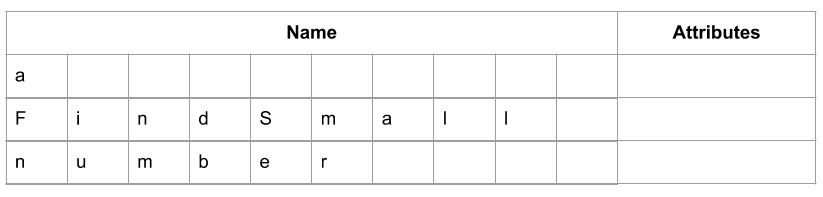
\includegraphics[width=\textwidth]{figures/FixedSize.png}
  \caption{This figure shows how the table can be formed using fixed sized field \cite{Dragon}}
  \label{fig:FixedSize}
\end{figure}
\begin{figure}[H]
\centering
  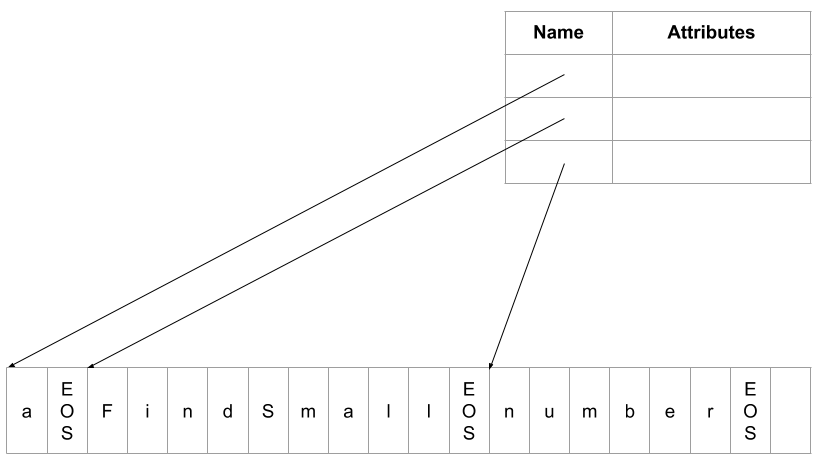
\includegraphics[width=\textwidth]{figures/InSeparateArray.png}
  \caption{This figure shows how the table can be formed using an separate array \cite{Dragon}}
  \label{fig:SeparateArray}
\end{figure}
\noindent
In PHAL the hash table approach was chosen, due to the better average case performance. This will be further elaborated upon in Chapter~\ref{ch:bindingvisitor}.
\chapter{Typechecking}\label{ch:typechecking}
In the following chapter the purpose of the type checker will be elaborated. 
The definition and function of a type system will be defined and explained in relation to PHAL. 
Furthermore, the differences between static and dynamic type checking will be analysed. 
Finally, the type conversions and operator overloading will be analysed and related to PHAL in general terms.

\section{Purpose of the type checker}
A compiler must check whether the source program follows both the syntactic and semantic conventions of the given language. 
This type of checking is called static type checking, and ensures that certain kinds of programming errors will be detected and reported. 
As indicated by Figure~\ref{fig:TypeChecker}, the type check takes place between the parsing and the intermediate code generation.
\begin{figure}[H]
\centering
  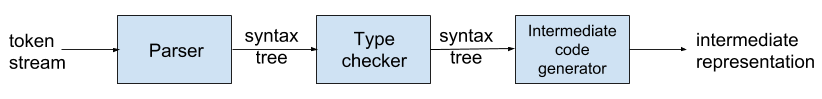
\includegraphics[width=0.8\textwidth]{figures/CompilerPhases/TypeChecker.png}
  \caption{This figure shows the position of the type checker in relation to the different compiler parses.}
  \label{fig:TypeChecker}
\end{figure}
The checks include, but are not limited to:
\begin{itemize}
    \item \textit{Type checks} - to see if an operation is applied to an incompatible operand.
    \item \textit{Flow-of-control checks} - statements that cause flow of control to leave a construct must have some place to transfer the flow of control.
    \item \textit{Uniqueness checks} - whether an object has been defined exactly once \cite{Dragon}.
\end{itemize}
If a given source program can pass the test of the type checker, it is said to be syntactically correct.

\section{Type systems}
When designing a type checker, multiple aspects of the language have to be considered, such as the syntactic constructs, the notation of types and rules for assigning types to language constructs. 

\subsection*{Type expressions}
The types of a language are denoted by type expressions. 
A type expression is either a basic type or is formed by applying an operator called a type constructor to other type expressions. 
The sets of basic types and constructors depend on the language that is subject to the check. 

\subsection*{Static and dynamic checking of types}
Type checking done at compile-time is called static type checking, whereas type checking done when the target program runs is called dynamic type checking.
If a language does not need dynamic type checking it is said to be \textit{sound}, because it allows us to statically determine that type errors can not occur on run time. 
\\\\
A language that is checked at compile time and can guarantee that the programs it accepts can be executed without any type errors is called a \textit{strongly typed} language \cite{Dragon}.

\subsection*{Error recovery}
Since the type checker has the potential to detect errors in the source program it needs the ability to take reasonable action when an error is discovered. At the very least the compiler should report the type and location of the error. However, it would be desirable for the type checker to be able to recover from an error and be able to check the rest of the program in order to detect any other potential errors before returning anything to the user.

\section{Type conversions}
During the type check it may be necessary to check conversions between types in most programming languages. 
Consider the expression $x+i$, where $x$ is of type \textit{integer} and $i$ is of type \textit{float}. In most languages it would be possible to convert $x$ to type \textit{float} since it would not result in missing precision.
\\\\
In PHAL this is mostly irrelevant since the abstraction of numbers has resulted in a single type to contain any kind of numbers. 
It would therefore not make sense to conduct type conversion in PHAL since \textit{integers} and \textit{floats} are the only similar data types.

\section{Overloading operators}
An overloaded symbol is one that takes on different meanings depending on the context in which it appears. 
For example, the $+$ is overloaded depending on context. In a mathematical context it would be used to imply addition of two numbers, however it can also be used on strings to perform a concatenation of them. In the same way, the dot operator is overloaded to either imply that a number is a \textit{float} or to access a \textit{sub-id} for an advanced type.
\\\\
The overloading of the $+$ operator in PHAL is described in Subsection~\ref{sem:aexp} and the other rules can be found in Appendix~\ref{app:semantics}.
\chapter{Code generation}\label{ch:CodeGenerationTheory}
The final phase of the compiler is the code generation phase.
When entering the code generation phase, the source program should have been transformed into an intermediate representation, usually in the form of an \textit{Abstract Syntax Tree} after passing through the previous phases of the compiler.
During this chapter, the goals and challenges associated with designing a code generator will be discussed. 
Furthermore, some of the techniques used in code optimisation will be introduced and discussed.

\section{The role of the code generator}
The role of the code generator is to produce the final output of the compiler based on the input program. This can take many different forms such as different types of machine languages or intermediate code \cite{Dragon}. 
\\\\
By compiling to machine language, the main advantage is that it can often be loaded directly into a fixed location in the memory of the device and can be executed immediately. This also has the advantage that small programs can be compiled and executed quickly \cite{Dragon}.
\\\\
However, compiling to another intermediate code is a widely used technique that makes use of previously written compilers to generate the executable code, decreasing the amount of work needed to be done when crafting a new compiler \cite{Dragon}.
\\
Several challenges can occur however when designing the code generator. 
These challenges must be kept in mind from the beginning, in order to create a successful code generator, and some of these challenges will be further described in this section.

%\subsection{Memory Management}
%Memory management problems can occur, depending on the output of the compiler. 
%The issue of memory management can be imminent when dealing with machine language programs since they %usually do not provide an easy way to deal with memory allocation and garbage collection.
%When the output of a compiler is in machine language, it is up to the designers of the code generator to keep track of memory allocation and garbage collection, otherwise the physical memory of the hardware platform might end up being filled.
%However, if the output of a compiler is in an intermediate code form, the memory management is usually handled by the compiler for the intermediate language.


%\subsection{Peephole optimisation}
%When trying to optimise code it is important to remember that optimised code is nothing more than that and should not be confused with optimal code.
%The purpose of optimised code is to reduce the overall running time \cite{Dragon}.
%\\\\
%A statement-by-statement approach applied in code generation will often result in target code containing redundant instructions \cite{Dragon}.
%A simple but effective technique for locally improving the target code is called \textit{peephole optimisation}. 
%The technique tries to improve the performance of the target program by examining a short sequence of instructions, called the peephole, and replacing the instructions with shorter or faster sequences whenever possible. 
%\\\\
%In the following subsections we will describe some of the easiest instructions to optimise \cite{Dragon}.

%\subsection{Unreachable code}
%One of the code sequences that is often easy to optimise is unreachable code. 
%To optimise unreachable code it simply needs to be eliminated. 
%The code generator has to determine whether parts of the code are unreachable, and therefore never executed. In this case it would make sense for the code generator to simply skip the excessive code bits.\\
%An example of unreachable code can be seen on listing~\ref{Code:UnreachableCode}
%\begin{lstlisting}[caption={Example of unreachable code}, label={Code:UnreachableCode}]
%lightbulb lamp := pin 1
%if (true is false) then
%{
%    lamp := on
%}
%\end{lstlisting}
%In Listing~\ref{Code:UnreachableCode}, the code generator should detect whether the condition of the %\textit{if}-statement is never going to be fulfilled, and conclude whether the entire In %\textit{if}-statement is unreachable and therefore not included in the target program.


%\subsection{Algebraic simplification}
%Another way to optimise the target program is to simplify algebraic expressions.
%Optimising algebraic expressions means that redundant algebraic expressions can be removed without altering the result. An example of this can be seen on Listing~\ref{Code:BadMath}.
%\begin{lstlisting}[caption={Example of an algebraic expression that can be optimised}, label={Code:BadMath}]
%x := x + 0
%or
%x := x * 1
%\end{lstlisting}
%In the listing both are legal expressions, but the results of the expressions have less complicated equivalents which can be be applied instead. In both examples, the right-most side of the expression can be ignored, without altering the result.

\section{Summary}
In this part, the usage of contextual grammar and the rules of the language have been defined, allowing the implementation of the compiler to begin.\\
In addition to this, the processes of a compiler have been theoretically described, and will be elaborated upon in the following part, where the theory will be supplemented with some code examples to further elaborate on how a compiler is crafted.


\part{Implementation}
\chapter{Main}
In the following chapters, the technical implementation of the PHAL language will be elaborated upon.
The first thing which we will introduce is the main class. 
\\\\
The main class is the piece of code from which the whole program starts and from which all the different compiler phases are executed. 
Apart from being the backbone of the program which connects all the different phases of the compiler, the main class is also used to store errors and warnings that have accumulated during the compiler phases. 
Errors and warnings are stored in the two lists shown on Listing~\ref{code:MainClassmain} on lines 2 and 3. The lists are regularly checked for errors that could end the compiling process. 
\\\\
As the program starts the program arguments are placed into member variables of the main class which is done on line 7 to 8 in Listing~\ref{code:MainClassmain}. 
It is important that the first argument is the name of the Phal file which the user wants to compile followed by a space, and then the specific USB port in which the Arduino board is connected to the users computer. 
An example of running the PHAL compiler can be seen on Listing~\ref{code:CommandToRunThePhalCompiler}.
\begin{lstlisting}[caption={Command to run the PHAL compiler}, label={code:CommandToRunThePhalCompiler}]
java -jar ./phal.jar PhalLangExample.phal COM4
\end{lstlisting}
The main class goes on to call the different parts of the compiler as seen on line 9 to 16 in Listing \ref{code:MainClassmain}, starting by building the abstract syntax tree, then instantiating the symbol table and then type checking. If no errors have occurred it will then proceed to code generation.
\begin{lstlisting}[caption={The main class},label={code:MainClassmain}, escapeinside={(*}{*)}]
public class MainClass {
  public static List<CompilerError.Error> CompileErrors = new ArrayList<>();
  public static List<CompilerError.Error> CompileWarnings = new ArrayList<>();
  (*\vdots*)
  public static void main(String args[]) throws Exception
  {
    inputFileName = args[0];
    String comPort = args[1];
    File file = new File(inputFileName);
    AstNode ast = ASTBuilder(new FileInputStream(file));
    SymbolTable ST = new SymbolTable();
    TypeChecking(ast, ST);	
    CodeGeneration cg = new CodeGeneration(ST.getCompInclMap());
    cg.visit((ProgramNode)ast);
    (*\vdots*)
  }
  (*\vdots*)
}
\end{lstlisting}
The first function call on Listing~\ref{code:MainClassmain} line 10 calls the function \textit{AstBuilder}.
\\
This function is responsible for creating the AST. 
To do this it first calls a couple of functions from the ANTLR framework which creates the concrete syntax tree.  
If no errors occur the AstBuilder will create an AST.
\\\\
After this the symbol table is created and the \textit{TypeChecking} function is called, as seen on line 12 in Listing \ref{code:MainClassmain}. 
The \textit{TypeChecking} function is shown in Listing \ref{code:MainClassTypechecking}.
\\
First the binding visitor, called on line 2, populates the symbol table and makes sure that variables and functions are declared before they are used as well as making sure that two variables are not declared with the same name. 
\\\\
Then the program checks if any errors occurred. 
If this is the case each error will be shown in the console window the user ran the program in and the program will terminate. 
This check is done after each phase or function is done as seen on line 4 to 6, 9 to 11 and 14 to 16 in Listing~\ref{code:MainClassTypechecking}.
\\\\
After the binding visitor the type checker is called. This phase makes sure that all interactions with variables and statements use the correct types.
\\
To finish this the type checking function the NumberVisitor is called as seen on line 12 in Listing \ref{code:MainClassTypechecking}. This functions checks for all number types whether they are integers or decimals. This is so code generation can be made more memory efficient which can be crucial on the very limited hardware in the Arduino.
\begin{lstlisting}[caption={The different checks needed to be done before code generation},label={code:MainClassTypechecking}, escapeinside={(*}{*)}]
public static void TypeChecking(AstNode ast, SymbolTable ST) {
  BindingVisitor bv = new BindingVisitor(ST);
  bv.visit((ProgramNode) ast);
  if(!CompileErrors.isEmpty()) {
    PrintErrorsAndExit();
  }
  TypeChecker tc = new TypeChecker(ST);
  tc.visit((ProgramNode) ast);
  if(!CompileErrors.isEmpty()) {
    PrintErrorsAndExit();
  }
  NumberVisitor nv = new NumberVisitor();
  nv.visit((ProgramNode) ast);
  if(!CompileErrors.isEmpty()) {
    PrintErrorsAndExit();
  }
  if(!CompileWarnings.isEmpty()) {
    PrintWarnings();
  }
}
\end{lstlisting}
After this process the compiler is now ready to start generating Arduino code which can then be compiled and uploaded to the Arduino board.
The following sections will further explain the implementation of how the AST is built, how the type checking is done, how numbers are evaluated to either integers or floats, and finally how the code generation is implemented.


\input{Worksheets/implementation/ErrorHandling.tex}
\chapter{Abstract Syntax Tree}
As described in Section~\ref{ca:ast}, an important part of crafting a compiler is generating an abstract syntax tree based on the source program, which can then be traversed to interpret the input.
 In this chapter the implementation of generating an AST will be explained, along with all the functionality hereof. 

\section{ANTLR4}
The first step of generating an AST for PHAL is to define the ANTLR4 grammar. 
This is largely equivalent to EBNF which is described in Section~\ref{sec:cfg}.
The main difference is that ANTLR uses slightly different notations for rules that can be repeated zero or more times. 
As seen on Listing~\ref{Code:ANTLRG41} line 4, an asterisk is used instead of curly brackets. 
Likewise, the colon symbol is used instead of an arrow to define the transition from the left side of the rule to the right.
\\
Finally, a semicolon is used to mark the end of a rule.

\begin{lstlisting}[caption={Part of Phal.g4}, label={Code:ANTLRG41}, escapeinside={(*}{*)}]
grammar Phal;

program
  : NEWLINE* include* setup NEWLINE* repeat NEWLINE* (func NEWLINE*)* NEWLINE* EOF ;
   
  (*\vdots*)

advDataType    
  : group | list;

cmpDcl    	
  : advType ID ':=' 'pin' NUMBER ( ',' NUMBER)* ;

  (*\vdots*)
\end{lstlisting}
As shown on Listing~\ref{Code:ANTLRG41} line 12 the keyword \textit{NUMBER} is used. 
Numbers, along with bool, comments, ID and others are defined at the buttom of the ANTLR4 file, as shown on Listing~\ref{Code:ANTLR4G42}

\begin{lstlisting}[caption={Part of Phal.g4}, label={Code:ANTLR4G42}, escapeinside={(*}{*)}]
(*\vdots*)
TEXT            : '"' ~('\r' | '\n' | '"')* '"' ;
ID              : LETTER (LETTER | DIGIT)*;
fragment INTEGER: DIGIT+;
fragment FLOAT  : (DIGIT | [1-9](DIGIT)+)'.'(DIGIT | (DIGIT)*[1-9]);
NUMBER          : (INTEGER | FLOAT) ;
BOOL            : ('true'|'false' | 'on' | 'off'); 

COMMENT         : '#' ~('\r' | '\n')*   -> skip ;
MULTILINECOMMET : '/*' .*? '*/'         -> skip ;
WS              : [ \t]+                -> channel(HIDDEN) ;
NEWLINE         : [\r\n];

fragment LETTER : [a-zA-Z];
fragment DIGIT  : '0'..'9';
\end{lstlisting}
This part of the implementation serves as a technical specification to ANTLR about how the types of PHAL should be interpreted.
\\\\
On line 3, \textit{TEXT} is defined as beginning with a quotation mark, followed by zero or more characters that can be anything but an end of line (\textbackslash r), new line (\textbackslash n) or a quotation mark (") and finally a quotation mark to finish the content of the text.
\\
On lines 5 and 6 the keyword \textit{fragment} is used, this implies that the integer and float types should never be used independently. 
Instead the fragments are used to define \textit{NUMBER} on line 7.
\\\\
This will later allow us to determine whether a number is a integer or a float, depending on which fragment was used.
Likewise, fragments are used for \textit{LETTER} and \textit{DIGIT} on lines 15 and 16.
Finally, it's worth looking at lines 10 and 11. 
For a single line comment, the right side of the rule is almost identical to how \textit{TEXT} was defined, with the exception that quotation marks are allowed in comments. 
The skip feature is used to instruct the lexer to discard the token.
\\\\
Having defined the grammar for ANTLR, it is now able to generate a lexer and parser, which can in turn generate a CST which is needed to build the AST that is needed to further advance trough the compile phases. 
The workings of ANTLR is further described in Subsection~\ref{ss:antlr}.

\section{Generating an AST from the CST}
As the CST generated from ANTLR contains a lot of information such as every character in the syntax. This means that if we have an if statement then the CST will include all the characters including the curly brackets and parentheses.
\begin{lstlisting}[caption={An if statement in PHAL}]
if(2 < 3) then {
  <statements>
}
\end{lstlisting}
This is irrelevant information for the compiler and slows down the process of working with the CST. It is therefore preferable to generate an abstract syntax tree instead.
\\\\
In order to accomplish this, a customised \textit{visitor} must be built, which inherits the properties of the automatically generated \textit{Base Visitor} from ANTLR.
\\\\
This class must contain methods to visit the nodes of the CST.
First of all we will take a look at \textit{Nodes} for the Phal language.
These are equivalent to the content of the CFG defined in Appendix~\ref{BNF:BNF}.
On Listings~\ref{EBNF:Program} and \ref{Code:Node:Program} a comparison of the node and EBNF for the root node called \textit{program} is shown.

\begin{lstlisting}[caption={EBNF for Program}, label={EBNF:Program}, escapeinside={(*}{*)}]
Program (*$\xrightarrow{}$*) {NEWLINE} {include} {NEWLINE} 
  Setup {NEWLINE} Repeat {NEWLINE} 
  {Func} {NEWLINE}
\end{lstlisting}

\begin{lstlisting}[caption={Node for Program}, label={Code:Node:Program}, escapeinside={(*}{*)}]
class ProgramNode extends AstNode{
  public SetupNode setupNode;
  public RepeatNode repeatNode;
  public List<FuncNode> funcNodes = new LinkedList<>();
  public List<IncludeNode> includeNodes = new LinkedList<>();
	
  public ProgramNode(List<IncludeNode> includeNodes, SetupNode setupNode, RepeatNode repeatNode, List<FuncNode> funcNodes) {
    this.includeNodes = includeNodes;
    this.setupNode = setupNode;
    this.repeatNode = repeatNode;
    this.funcNodes = funcNodes;
  }
}
\end{lstlisting}
Since the semantic rules specify that a program must contain exactly one setup and one repeat, it must include exactly one of each node in the \textit{ProgramNode}.
\\\\
In order to facilitate the case where a program contains multiple includes or func declarations, a linked list is used.
\\\\
Finally, each node contains a constructor in order to generate the node.

\subsection*{The type node}
Some nodes are slightly different from the default construction described above. For example the \textit{type} node. 
\begin{lstlisting}[caption={EBNF for Type}, label={EBNF:Type}, escapeinside={(*}{*)}]
type        
  : 'number' | 'text' | 'bool' | 'list' | 'group' | advType;
  
advDataType    
  : group | list;
\end{lstlisting}

\begin{lstlisting}[caption={Node for Type}, label={Code:Node:Type}, escapeinside={(*}{*)}]
class TypeNode extends AstNode{
  public String type;
  public Type Type;
	
  public TypeNode(String type) {
    this.type = type;
	
    switch(this.type) {
    case "number":
      this.Type = Type.NUMBER;
      break;
    case "text":
      this.Type = Type.TEXT;
      break;
    (*\vdots*)
    case "motor":
      this.Type = Type.MOTOR;
      break;
    case "temperaturesensor":
      this.Type = Type.TEMPERATURESENSOR;
      break;
    case "none":
      this.Type = Type.NONE;
      break;
    }
  }
}

enum Type{
  NUMBER, TEXT, BOOL, GROUP, LIST, LIGHTBULB, 
  MOTOR, TEMPERATURESENSOR, NONE
}
\end{lstlisting}
The \textit{Type} node is a universal node used for all types of variables. Due to this, it requires a \textit{String} for the constructor, in order to properly assign the correct type to the node.
The \textit{String} is interpreted using a switch statement, and is then assigned a \textit{Type}, which is defined as an enumerator. 


\subsection{The AST builder}
Having defined the entire set of nodes, it is now possible to traverse through the CST and build an AST with the new node types.\\
As previously mentioned, this will be done using a custom implementation of the visitor generated by ANTLR.


\begin{lstlisting}[caption={Code for visitProgram}, label={Code:visitProgram}, escapeinside={(*}{*)}]
@Override
public AstNode visitProgram(PhalParser.ProgramContext ctx) {
  SetupNode setupNode = null;
  RepeatNode repeatNode = null;
  List<FuncNode> funcNodes = new LinkedList<>();
  List<IncludeNode> includeNodes = new LinkedList<>();
	
  if(ctx.setup() != null)
  {
    setupNode = (SetupNode)visit(ctx.setup());
  }
  if(ctx.repeat() != null)
  {
    repeatNode = (RepeatNode)visit(ctx.repeat());
  }
  for(PhalParser.FuncContext func: ctx.func()) 
  {
    funcNodes.add((FuncNode) visit(func));
  }
  for(PhalParser.IncludeContext include: ctx.include()) 
  {
    includeNodes.add((IncludeNode) visit(include));
  }
  return new ProgramNode(includeNodes, setupNode, repeatNode,funcNodes);
}
\end{lstlisting}
The implementation of the AST builder is very simple. If there is a single node of the given type, such as setup and repeat, the method has to ensure that the given node is not null in the CST, visit it using the visitor method generated by ANTLR and assign the result to the correct internal node.
\\\\
As in the main node, for each internal node that has zero or more instances a linked list is used. This list is iterated through using a for-loop, where it will call the visitor on each member for the list.


\chapter{Binding visitor}\label{ch:bindingvisitor}
In this chapter we will take a look at the binding visitor and how we used the symbol table to bind assignments and expressions to their declarations.
The binding visitor's functionality is to ensure that there are not multiple variables with the same name, and that variables that are used in assignments and statements are declared before use. The binding visitor is also used to decorate the AST. All references to a variable are decorated with their declaration node to make it possible to type check all assignments and expressions in the type checker.

\section{Symbol table}
As mentioned in Chapter~\ref{ch:symboltable}, a symbol table is used to map out which variables are declared in the current scope. We chose to implement the symbol table as a class, which can be seen on Listing~\ref{code:SymbolTableClass}.
\begin{lstlisting}[caption={Symbol table class},label={code:SymbolTableClass}]
private HashMap<String, FuncNode> functionMap = new HashMap<>();
private Stack<HashMap<String, AstNode>> symbolTable = new Stack<>();
\end{lstlisting}
The \textit{SymbolTable} class contains a stack of hashmaps. 
This is the symbol table where each hashmap in the stack represents a scope. 
The class also contains a hashmap with all of the defined functions called \textit{functionMap}. 
This map is used to easily open scopes with the different functions when they are called.
The \textit{SymbolTable} class also contains a couple of functions that handle the different functionalities of the symbol table. 
\begin{lstlisting}[caption={Code to open and close scopes},label={code:OpenCloseScope}]
public void openScope() {
  this.symbolTable.push(new HashMap<String, AstNode>());
}
public void closeScope() {
  this.symbolTable.pop();
}
\end{lstlisting}
As shown on Listing~\ref{code:OpenCloseScope} are the functions that are used to open and close scopes. The function \textit{openScope} pushes a new hashmap to the stack. This is used when functions are called. The function \textit{closeScope} pops the hashmap on top of the stack. 

\begin{lstlisting}[caption={Code to add declaration to the symbol table},label={code:AddToSymbolTable}]
public void addDeclarationToSymbolTable(DclNode node) {
  if(symbolTable.peek().containsKey(node.idNode.id))
  {
    MainClass.CompileErrors.add(new RedeclarationError(
                            node.columnNumber, 
                            node.lineNumber, 
                            node.idNode.id));
  }
  else
  {
    symbolTable.peek().put(node.idNode.id, node);
  }
}

public void addAssignmentToSymbolTable(AssignmentNode node) {
  HashMap<String, AstNode> map =  symbolTable.peek();
  String key = node.idNode.id;
		
  if(map.containsKey(key))
  {
    DclNode dcl = (DclNode)map.get(key);
    if(!dcl.isUsed) {
      dcl.isUsed = true;
      map.put(key, dcl);
    }
    node.idNode.dclNode = dcl;
  }
  else
  {
    MainClass.CompileErrors.add(new NotDeclaredError(
                           node.columnNumber, 
                           node.lineNumber, 
                           node.idNode.id));
  }
}
\end{lstlisting}
The \textit{addDeclarationToSymbolTable} method shown on Listing~\ref{code:AddToSymbolTable} lines 1-13 is used to add declarations to the symbol table. 
It starts by checking if the declaration already exists in the symbol table, in which case an error is added to the error list and the program will continue. 
If the declaration does not already exist in the symbol table it is added by adding the \textit{DclNode} to the symbol table with its \textit{id} as the key in the hashmap.
\\\\
The second method, \textit{addAssignmentToSymbolTable} as shown on Listing~\ref{code:AddToSymbolTable} lines 15-35, checks whether or not the variable you are trying to assign is declared. 
This is done by checking if the hashmap contains the key (id) of the \textit{AssignmentNode}. 
\\\\
In this case, it checks whether the \textit{isUsed} flag of the \textit{DclNode} in the hashmap is flagged as true.
\\\\
If this is not the case, it is set to true and the \textit{DclNode} gets put into the hashmap again, which means that it overrides the old \textit{DclNode}. 
After this, the \textit{DclNode} is added to the \textit{AssignmentNode}. This is done to decorate the AST to allow it to be type checked later on.
\\\\
However, if the hashmap does not contain the id of the \textit{AssignmentNode} a new error is added to the error list and the program continues.
There are more \textit{addToSymbolTable} functions, which have the same structure but contain different node types. 
\begin{lstlisting}[caption={Code to check if variables are used}, label={code:checkVariablesAreUsed}]
public void checkVariablesAreUsed() {
  for(AstNode node : symbolTable.peek().values()) {
    if(node instanceof DclNode) {
      if(!((DclNode) node).isUsed) {
        MainClass.CompileWarnings.add(
          new VarNotUsedWarning(node.columnNumber, 
          node.lineNumber, ((DclNode) node).idNode.id));
      }
    }
  } 
}
\end{lstlisting}
The \textit{checkVariablesAreUsed} method, shown on Listing~\ref{code:checkVariablesAreUsed}, checks if any of the variables that are declared in the symbol table are ever used in the code. 
It does so by iterating through each element in the symbol table and checking whether the \textit{isUsed} flag is marked as true or false. 
If they are marked as false we add a warning to the warning list in order to warn the user that they have some variables that might be unnecessary.

\section{Binding visitor}
As mentioned previously in this chapter, the binding visitor's functionality is to traverse through the AST nodes, add all declarations to the symbol table and check if any of the assignments, statements or expressions use any ids that are not declared prior to being used.
\begin{lstlisting}[caption={Code for the binding visitor}, label={code:BindingVisitorClass}]
public class BindingVisitor extends Visitor {
  public SymbolTable ST = null;
	
  public BindingVisitor(SymbolTable symT) {
    ST = symT;
    ST.openScope();
  }
}
\end{lstlisting}
The \textit{BindingVisitor}, shown on Listing~\ref{code:BindingVisitorClass}, inherits from the \textit{Visitor} class and uses the visitor pattern, as described in Subsection~\ref{comp:VisitorPattern}, to traverse the AST and bind ids to declarations. It contains an instance of the \textit{SymbolTable} class and uses this to keep track of all the functions and which variables are declared in the current scope as can be seen on Listing~\ref{code:BindingVisitorCall}.

\begin{lstlisting}[caption={Code for binding visitor call}, label={code:BindingVisitorCall}]
SymbolTable ST = new SymbolTable();
BindingVisitor bv = new BindingVisitor(ST);
bv.visit((ProgramNode) ast);
\end{lstlisting}
When the \textit{BindingVisitor} is instantiated it takes a symbol table as a parameter. Following this the visit function is used to visit the \textit{ProgramNode} of our AST.

\begin{lstlisting}[caption={Code for the ProgramNode visitor}, label={code:BindingVisitorProgramNode}]
public void visit(ProgramNode node)
{
  /*Creates FunctionMap*/
  if(node.funcNodes != null)
  {
    for(FuncNode func: node.funcNodes)
    {
      ST.addToFuncMap(func);
    } 
  }
  /*Creates ST*/
  node.setupNode.accept(this);
  node.repeatNode.accept(this);
  ST.checkVariablesAreUsed();
		
  if(node.funcNodes != null)
  {
    for(FuncNode func: node.funcNodes) {
      func.accept(this);
    }
  }
  ST.checkFunctionsAreUsed();
}
\end{lstlisting}
When the \textit{ProgramNode} is visited it first iterates through all the functions and adds them to the SymbolTable as shown on Listing~\ref{code:BindingVisitorProgramNode}. It then uses the visitor to visit the \textit{SetupNode} and the \textit{RepeatNode} within the \textit{ProgramNode}.
Afterwards it checks whether there are any variables that are declared but never used. In this case it adds a warning to the warning list.
Afterwards it iterates through all the \textit{FuncNode}s and visits them. After this it checks whether there are any functions that were defined but never used. 
\begin{lstlisting}[caption={Code for the VarDcl visitor}, label={code:VarDclNodeVisitor}]
public void visit(VarDclNode node)
{
  ST.addDeclarationToSymbolTable(node);
  if(node.exprNode != null) {
    node.isInitialized = true;
    node.exprNode.accept(this);
  }
}
\end{lstlisting}
When visiting a \textit{DclNode}, it starts by adding the declaration to the \textit{SymbolTable} as shown on Listing~\ref{code:VarDclNodeVisitor}. It checks whether the \textit{ExpressionNode} is \textit{null}. If it is not, it sets the \textit{isInitalized} flag on the \textit{DclNode} to be true, meaning that the \textit{decleration} is set to a value.

\begin{lstlisting}[caption={Code for the ListNode visitor}, label={code:ListNodeVisitor}]
public void visit(ListNode node)
{
  ST.addDeclarationToSymbolTable(node);
  node.isInitialized = true;
  node.typeNode.accept(this);
  if(node.memberExprNodes != null)
  {
    for(ExprNode expr: node.memberExprNodes)
    {
      expr.accept(this);
    }
  }
}

@Override
public void visit(GroupNode node)
{
  ST.addDeclarationToSymbolTable(node);
  node.isInitialized = true;
  for(IdNode member: node.memberIdNodes) 
  {
    member.accept(this);
  }
}
\end{lstlisting}
\textit{List} and \textit{Group} declarations are different because they contain multiple members. When visiting these, the function first adds the \textit{declaration} to the \textit{SymbolTable}. Then it iterates through all the members and visits them as can be seen on Listing~\ref{code:ListNodeVisitor}.

\begin{lstlisting}[caption={Code for the AssignmentNode visitor}, label={code:AssignmentNodeVisitor}]
public void visit(AssignmentNode node)
{
  ST.addAssignmentToSymbolTable(node);
  node.idNode.dclNode.isInitialized = true;
  node.exprNode.accept(this);
}

public void visit(IdNode node) {
  ST.addIdToSymbolTable(node);
  if(node.dclNode != null && node.dclNode.isInitialized == false) {
    MainClass.CompileWarnings.add(
                              new NotInitializedWarning(
                                node.columnNumber, 
                                node.lineNumber, 
                                node.id)
                                );
  }
}
\end{lstlisting}
When visiting an \textit{AssignmentNode}, the visit function adds the assignment to the symbol table and sets the \textit{idInitialized} flag to true, as can be seen on Listing~\ref{code:AssignmentNodeVisitor} line 4 followed by visiting the \textit{ExpressionNode}.
\\\\
When visiting an \textit{IdNode}, the function adds the id to the symbol table as shown on Listing~\ref{code:AssignmentNodeVisitor} lines 8-18. 
This checks whether or not the is declared. 
Then the \textit{DclNode} is checked for whether the \textit{IdNode} is \textit{null}. 
If so, the \textit{isInitializedflag} on the \textit{DclNode} is set to false. 
If it is true, it adds a warning to the warning list to inform the user that a variable is not initialised.


\chapter{Type checker}\label{ch:TypeCheckerImplimentation}
The type checker class is responsible for making sure that the program variables and expressions have the correct types throughout the program. First of all, it inherits from the \textit{Visitor} class to enable traversal of the AST. Every node in the AST that needs to be type checked then has their visit method overridden to implement the type checking code for each of the different nodes. The type checker is purely based on \textit{visit} methods, and they are not that different in terms of implementation. As such, a few examples are shown to give an idea of the general implementation procedure.

\begin{lstlisting}[caption={Type checking for functions}, label={code:FuncNodeTypeChecking}]
@Override
public void visit(FuncNode funcNode) {
  super.visit(funcNode);
  for(int i = 0; i < funcNode.funcCntNodes.size(); i++) {
    if(funcNode.funcCntNodes.get(i)
    .stmtNode instanceof ReturnStmtNode) {
      ReturnStmtNode rsNode = (ReturnStmtNode) 
      funcNode.funcCntNodes.get(i).stmtNode;
			
      visit(rsNode.exprNode);
			
      if(rsNode.exprNode.type != funcNode.typeNode.Type) {
        // Type error
      }
      else if(isAList(rsNode.exprNode)
      && !funcNode.typeNode.islist) {
        // List error
      }
      else if(!isAList(rsNode.exprNode) 
      && funcNode.typeNode.islist) {
        // List error
      }
    }
  }
}
\end{lstlisting}
The \textit{visit} method on Listing~\ref{code:FuncNodeTypeChecking} is responsible for type checking functions.
This includes checking if each of the return statements inside the function are the same type as the function's specified return type. 
Furthermore, this ensures that the functions return type and the return statements are both either lists or that none of them are lists. 
\\\\
First of all, the \textit{visit} method from the \textit{Visitor} class is called with the \textit{super.visit(funcNode)} method on line 3 to make sure that all statements and declarations inside the function are being visited. 
After this, the for loop on line 4 is used to check each \textit{stmtNode} object in the function body if any of them are return statements. 
If the check returns true, a \textit{ReturnStmtNode} object is instantiated by typecasting the specific \textit{stmtNode} on line 7-8.
\\\\
The visit method for the return statement is then called on line 10 to ensure that its type has been evaluated. It is then checked whether the type of this return statement is the same as the function's return type. If not, a type error is added to the \textit{MainClass} (represented by the comment on line 13). If the types are correct, we then need to check if the statement is a list and the return type of the function is not a list. We do not want it to be possible to return a list in function that does not expect a list, nor do we want it to be possible to return an expressions that is not a list in a function that expects a list. An error will be written if this is the case, which can be seen on line 17 and 21.

\begin{lstlisting}[caption={Type checking for loop until}, label={code:LoopUntilTypeChecking}]
@Override
public void visit(LoopUntilNode node) {
  super.visit(node);
  checkCondition(node.exprNode);
		
  if(node.idNode.type != Type.NUMBER) {
    // Type error
  }
}

private void checkCondition(ExprNode expr) {
  if(isAList(expr)) {
    // List error
  }
  if(expr.type != Type.BOOL) {
    // Type Error
  }
}
\end{lstlisting}
For the type checking of a \textit{loop-until} structure (Listing~\ref{code:LoopUntilTypeChecking}), it must be ensured that the expression in the condition is of type \textit{boolean}. 
We also need to check that identifier that is incremented/decremented by of type \textit{number}. 
Firstly, the \textit{visit} from the \textit{Visitor} is called with the \textit{super} keyword on line 3 to visit all the content of the \textit{LoopUntilNode} so that this can be type checked as well. 
Then the condition is checked by calling the \textit{checkCondition} method. 
\\\\
This method will first of all check if the expression in the condition is a list, because this should not be possible, and will therefore write a list error (line 13). 
The method then checks if the type of the expression is a \textit{boolean} (line 15). 
If it is not, a type error is issued. 
It is then checked if the type of the identifier that is incremented/decremented is a number, and if it is not, an error is once again issued to the \textit{MainClass}.

\begin{lstlisting}[caption={Type checking for function calls as expressions}, label={code:funcCallExprTypeChecking}]
@Override
public void visit(FuncExprNode funcExprNode) {
  ParametersNode formalParams = st.getFunctionFromFuncMap(
  funcExprNode.funcCallNode).parametersNode;

  checkActualAndFormalParams(funcExprNode.funcCallNode, 
  funcExprNode.funcCallNode.callCntNode, formalParams);

  funcExprNode.type = st.getFunctionFromFuncMap(funcExprNode
  .funcCallNode).typeNode.Type;
}
\end{lstlisting}
When type checking function calls (Listing \ref{code:funcCallExprTypeChecking}), the idea is to make sure that the actual parameters that have been input to the function are compatible with the formal parameters defined in the function declaration. 
In this \textit{visit} method the symbol table is used to look up the specific function on line 3-5, and the \textit{parametersNode} from the call to the symbol table, which contains all of the formal parameters for the function, is saved in a new object \textit{formalParams}. 
\\\\
This node, together with the \textit{funcCallNode}, which contains the actual parameters, is then passed to the method \textit{checkActualAndFormalParams} on line 7-8 which will do the type checking and make sure the the actual parameter types are compatible with the types of the formal parameters. 
It will also make sure that the correct number of parameters have been given to the function call. 
Finally, the \textit{funcExprNode} needs to have a type so it can be used in an expression. This type is the return type of the function, which is looked up in the symbol table on line 11-12 and assigned to the expression.
\chapter{Number Visitor}
PHAL includes the \textit{number} type. \textit{Number} is a type that, when compiled down to APL, can either be an integer or a decimal depending on the context. The \textit{number} therefore needs to be evaluated to decide whether it compiles to an integer (\textit{int}) or a decimal (\textit{float}). This means that we have to visit all instances where a \textit{number} can be present such as variable declarations, assignments and function calls to check whether the \textit{number} is an integer or not.

\section{Visitor}
The \textit{Number Visitor} inherits the visitor pattern from the \textit{Visitor} class and overrides some of the \textit{visit} methods to implement the \textit{Number Visitor}'s functionality. Inheriting from the \textit{Visitor} means that it will traverse the AST node for node through the \textit{visit} methods.
\\\\
In the following subsections we will take a closer look at a few of these methods. The methods that are chosen are for the program node, which is the root of the AST, the variable declaration nodes, the assignment nodes and the function nodes. The \textit{ProgramNode} \textit{visit} is shown because it is used to map all of the functions, and it also contains all the nodes. Variable declarations, assignments and functions are described here because they can contain numbers that needs to be evaluated.

\subsection{ProgramNode}
The first thing that happens is that a hashmap is created containing all the functions (\textit{FuncNodes}) as shown on Listing~\ref{code:NumberVisitor:VisitProgramNode} line 1. This is done to easily access the declarations (\textit{DclNodes}) of the formal parameters of functions that are called throughout a program. 
If the function is ever called with a \textit{float} as an actual parameter then the corresponding formel parameter has to be declared as a \textit{float} in the intermediate generated code, in this case APL.
We then use the \textit{super.visit()} to visit the \textit{Visitors} implementation of this method, which will visit all the \textit{ProgramNode's} children. 

\begin{lstlisting}[caption={code to implement the ProgramNode visitor and function map}, label={code:NumberVisitor:VisitProgramNode}]
private HashMap<String, FuncNode> functionMap = new HashMap<>();
@Override
public  void visit(ProgramNode node){
  for(FuncNode func : node.funcNodes){
     functionMap.put(func.idNode.id, func);
  }
  super.visit(node);
}
\end{lstlisting}
\subsection{VarDclNode}
When visiting Variable declarations (\textit{VarDclNodes}), it is first checked if the variable's type is a \textit{number} as shown on Listing~\ref{code:NumberVisitor:VisitVarDclNode} line 2. 
\\
If the variable is of the type \textit{number} it is checked whether the variable is assigned a value. This is done by checking if the expression node (\textit{ExprNode}) is null, if the expression is not null it means that the variable was declared and assigned to a value and further checks need to be done.
\\
If the variable is a number and it gets assigned a value, then the \textit{VarDclNode's} member variable \textit{isInt} is set equal to the boolean result returning from the method \textit{checkExprType}. This method takes the \textit{VarDclNode's} \textit{ExprNode} as a parameter and evaluates whether all occurrences of numbers in this expression are of the type integer or float.
\\
The \textit{checkExprType} returns \textit{false} if a \textit{float} number ever occurs in the \textit{ExprNode} and \textit{true} if all the numbers are a \textit{integer}. The method's use is shown on line 3.

\begin{lstlisting}[caption={code to implement the VarDclNode visitor}, label={code:NumberVisitor:VisitVarDclNode}]
public void visit(VarDclNode node) {
  if(node.typeNode.Type == Type.NUMBER && node.exprNode != null) {
    node.typeNode.isInt = checkExprType(node.exprNode);
  }
}
\end{lstlisting}

\subsection{AssignmentNode}
When visiting an assignment (\textit{AssignmentNode}) it is first checked if the variable that is being assigned to is of the type \textit{number}, as shown on Listing~\ref{code:NumberVisitor:VisitAssignmentNode} line 2. 
\\
If the variable is of the type \textit{number} we check what type of declaration the variable was by using the \textit{instanceof} keyword to get the derived class from the abstract class \textit{DclNode}.
In this situation it can either be an instance of a variable declaration (\textit{VarDclNode}) or a formal parameter (\textit{ParamNode}).
\\\\
The reason for this check is that the \textit{DclNode} class does not contain a \textit{TypeNode} and the \textit{TypeNode} is where we have the \textit{isInt} flag on. The isInt flag is placed on the TypeNode to make it easier for the CodeGenerator to access when generating the declarations
Then the \textit{DclNode} is explicitly casted to either a \textit{VarDclNode} or a \textit{ParamnNode} depending on which one it is an instance of. 
\\\\
We then check if the \textit{isInt} flag on the now casted \textit{DclNode} is \textit{true} or \textit{false} on line 5. 
If it is \textit{true} then we set the \textit{isInt} flag equal to the result of \textit{checkExprType}, in the same way as it was done in listing \ref{code:NumberVisitor:VisitVarDclNode}. 
It will return \textit{false} if the \textit{exprNode} contains a \textit{float} and \textit{true} if it only contains \textit{intergers}.
\\\\
If the \textit{isInt} flag is \textit{false} we do nothing because this means that it is a \textit{float} and a \textit{float} can not be converted to an \textit{integer} without losing precision.

\begin{lstlisting}[caption={code to implement the AssignmentNode visitor}, label={code:NumberVisitor:VisitAssignmentNode}]
public void visit(AssignmentNode node) {
  if(node.idNode.type == Type.NUMBER) {
    if(node.idNode.dclNode instanceof VarDclNode) {
      VarDclNode dcl = (VarDclNode) node.idNode.dclNode;
      if(dcl.typeNode.isInt) {
        dcl.typeNode.isInt = checkExprType(node.exprNode);
      }
    } else {
        ParamNode dcl = (ParamNode) node.idNode.dclNode;
        if (dcl.typeNode.isInt) {
          dcl.typeNode.isInt = checkExprType(node.exprNode);
        }
    }
  }
}
\end{lstlisting}


\subsection{FuncCallNode}
When visiting a function call(\textit{FuncCallNode}) we first check whether there are any actual parameters. If there are no actual parameters then nothing happens. But if there are any then the corresponding \textit{FuncNode} from the hashmap that we created when visiting the \textit{ProgramNode}, as shown in Listing~\ref{code:NumberVisitor:VisitProgramNode}, is extracted and saved in a local variable.
\\\\
Then the formal parameters \textit{isInt} flag, from from the \textit{FuncNode}, is evaluated based on the corresponding actual parameters. This is done by setting the \textit{isInt} flag from the formal paramters equal to the return value from the method \textit{CheckExprType} where the expression node being passed as its parameter is equal to the corresponding actual parameter.
\\\\
If the \textit{ExprNode} only contained \textit{integers} the \textit{CheckExprType} returns \textit{true}, but if the \textit{ExprNode} contained any \textit{floats} then \textit{CheckExprType} returns \textit{false} and the corresponding parameter is declared as a \textit{float} when the function is declared in APL. 
\begin{lstlisting}[caption={code to implement the FuncCallNode visitor}, label={code:NumberVisitor:VisitFuncCallNode}]
public void visit(FuncCallNode node) {
  if(node.callCntNode != null) {
    FuncNode func = functionMap.get(node.idNode.id);
    for(int i = 0; i < node.callCntNode.exprNodes.size(); i++){
      if(func.parametersNode.paramNodes.get(i).typeNode.isInt){
        func.parametersNode.paramNodes.get(i).typeNode.isInt = checkExprType(node.callCntNode.exprNodes.get(i));
      }
    }
  }
}
\end{lstlisting}

\section{CheckExprType}
To check whether an \textit{ExprNode} contains \textit{floats}, we made use of method overloading by imitating the \textit{Visitor} pattern. 
We implemented a \textit{CheckExprType} method for each derived class of the \textit{ExprNode}. 
We then made use of recursive calls to handle the different contents of the \textit{ExprNodes}.

\subsection{IdRefExprNode}
An \textit{IdRefExprNode} is a reference to an already declared variable. 
When checking if the \textit{IdRefExprNode} is a \textit{float} or an \textit{int} we just return the \textit{isInt} flag from \textit{typeNode} on the \textit{DclNode} on the \textit{IdRefExprNode} as can be seen on Listing~\ref{code:NumberVisitor:IdRefExprNode}.
\begin{lstlisting}[caption={This listing shows the checkExprType method}, label={code:NumberVisitor:IdRefExprNode}]
private boolean checkExprType(IdRefExprNode node) {
  if(node.idNode.dclNode instanceof VarDclNode) {
    return ((VarDclNode) node.idNode.dclNode).typeNode.isInt;
  } else {
    return ((ParamNode) node.idNode.dclNode).typeNode.isInt;
  }
}
\end{lstlisting}

\subsection{LiteralExprNode}
A \textit{LiteralExprNode} is a \textit{ExprNode} that contains a literal. 
This means that in this context it will contain a string with a number in it. 
To check if it is a \textit{integer} or a \textit{float} we try to parse it as a \textit{integer}. 
\\\\
Since we have already been through the type checker we can be surden that the \textit{LiteralExprNode's} type is number.
If it throws an exception we know that it is a \textit{float} and we return \textit{false}.
\\\\
If it does not throw an exception we know that it is an \textit{integer} and we return \textit{true} as can be seen on Listing~\ref{code:NumberVisitor:LiteralExprNode}.
\begin{lstlisting}[caption={Code to implement the checkExprType method that takes a LiteralExprNode as a parameter}, label={code:NumberVisitor:LiteralExprNode}]
private boolean checkExprType(LiteralExprNode node){
  try {
    Integer.parseInt(node.literalExprNode);
  } catch (NumberFormatException e) {
    return false;
  }
  return true;
}
\end{lstlisting}
The remaining types of \textit{ExprNode}s simply contain one or more \textit{ExprNode}s, and are checked recursively. \\
Following the completion of the number visitor, the source code has now been analysed and type checked, and is prepared for the final phase, code generation, which will be further described in the next chapter.
\chapter{Code generation}
The code generation is the final phase of the compiler, it is responsible for traversal of the AST and generating the appropriate APL code. 
Doing this chapter we will look at the different overrides of the visit methods responsible for generating the APL code.
\\\\
The code generation class inherits from the visitor class to enable the traversal of the AST, just like the type checker. Every node of the AST must be visited in order to generate the corresponding code in APL. The first listing to look at is the one for a whole program.

\begin{lstlisting}[caption={Code generator for a program}, label={code:CodeGeneratorVisit}]
@Override
public void visit(ProgramNode node) {
  printHeader();
  printCmpIncludes();

  for (IncludeNode incl : node.includeNodes) {
    visit(incl);
  }
  for (SetupCntNode dcl : node.setupNode.setupCntNodes) {
    if (dcl.dclNode instanceof VarDclNode) {
      visit((VarDclNode) dcl.dclNode, CodeGen.GLOBAL);
    }
    if (dcl.dclNode instanceof ListNode) {
      visit((ListNode) dcl.dclNode, CodeGen.GLOBAL);
    }
    if (dcl.dclNode instanceof GroupNode) {
      visit((GroupNode) dcl.dclNode, CodeGen.GLOBAL);
    }
    if (dcl.dclNode instanceof CmpDclNode) {
      visit((CmpDclNode) dcl.dclNode, CodeGen.GLOBAL);
    }
  }

  visit(node.setupNode);
  visit(node.repeatNode);

  for (FuncNode func : node.funcNodes) {
    visit(func);
  }
  writer.close();
}
\end{lstlisting}
Listing~\ref{code:CodeGeneratorVisit} is responsible for checking the strcuture of the program and calling the approriate visit methods to convert from PHAL to APL based on note types.
On Listing~ line 3, the header of the APL file is added to state that the code is generated by the PHAL compiler stating the date of compilation. 
Line 4 simply writes the includes to the output file. The for loop starting on line 9 if used for declaring variables globally. After global variables have been generated, this method calls the visit methods for setup part of the program, then the repeat part and finally the function declarations that end the general structure of a PHAL program. Once every part of the program is visited, link 29 closes the writer, meaning the program has finished compilation.

\begin{lstlisting}[caption={Generating code for a variable declaration }, label={code:CodeGenVarDcl}]
public void visit(VarDclNode node, Enum<CodeGen> location) {
  if (location == CodeGen.GLOBAL) {
    visit(node.typeNode);
    writer.print(" ");
    visit(node.idNode);
  }

  if (location == CodeGen.SETUP) {
    if (node.exprNode != null) {
      visit(node.idNode);
      writer.print(" = ");
      visit(node.exprNode);
    }
  }

  if (location == CodeGen.FUNCTION) {
    visit(node.typeNode);
    writer.print(" ");
    visit(node.idNode);
    if (node.exprNode != null) {
      writer.print(" = ");
      visit(node.exprNode);
    }
  }
  writer.print(";\n");
}
\end{lstlisting}
To generate code for declarations, the location where they appear must be taken into account. As shown in the for loop on Listing~\ref{code:CodeGeneratorVisit} line 9, the location is given as input through a CodeGen enum. This location is then used in the code shown in Listing~\ref{code:CodeGenVarDcl} to determine how the code is generated. If the location is global, it visits the type node to generate the type, prints a space and then generates the identifier. The variables in setup are defined through the global scope, but initialised in setup, which is why variables with that location do not visit the \textit{typeNode}. If the variable is declared in a function, it must check the type and initialise. 

\begin{lstlisting}[caption={Generating code for the repeat section of PHAL}, label={code:ReapeatGen}]
@Override
public void visit(RepeatNode node) {
  writer.print("void loop(){ \n");
  super.visit(node);
  writer.print("} \n\n");
}
\end{lstlisting}
The APL equivalent to our repeat is loop. Therefore, when generating code for the RepeatNode we generate the loop function. Inside the loop functions block we use the \textit{super.visit} to call the visitor function of the visitor class. This is done to prevent code duplication because the visit function in the Visitor class that takes the RepeatNode as parameter already visits all its contents.
\begin{lstlisting}[caption={Generating code for an assignment statement}, label={code:AssignStatement}, escapeinside={(*}{*)}]
@Override
public void visit(AssignmentNode node) {
  if (node.idNode.type == Type.GROUP) {
    if (node.assignmentOperator == AssignmentOperator.EQUALS) {
      visit(node.idNode);
      LiteralExprNode le = (LiteralExprNode) node.exprNode;

      switch (le.literalExprNode) {
        case "true":
        case "on":
          writer.print(".on();\n");
          break;
        (*\vdots*)
      }
    }
  } 
  (*\vdots*)
  else {
    visit(node.idNode);
    if (node.assignmentOperator == AssignmentOperator.EQUALS) {
      writer.print(" = ");
    } else {
      writer.print(node.assignmentOperator.toString());
    }
    visit(node.exprNode);
    writer.print(";\n");
  }
}
\end{lstlisting}
The assignment statements shown in Listing~\ref{code:AssignStatement} differ based on the type that is assigned to. 
Groups and list require different implementation than the basic types: text, number and bool that are assigned to through in the same way. 
This means the first thing to check is the type of the node given as a parameter. 
For groups, the next thing to check is whether the operator used for assignment is equal to the one defined for assignments in the \textit{AssignmentOperator} enumeration type, as seen on line 4. 
\\\\
If the syntax is correct, it visits the node, converts it to a literal expression node, and switches what to print based on the boolean value or its alias. 
\\\\
If the node is of any other type than list or group, the generator either prints an equal sign or the value of the \textit{assignmentOperator} on the node as a string. 
Finally, on line 25 the expression is visited and a semicolon is printed to conform to the APL rule for ending statements.

\begin{lstlisting}[caption={Generating code for an if-statement}, label={code:IfStatement}]
@Override
public void visit(IfStmtNode node) {
  writer.write("if(");
  visit(node.ifExprNode);
  writer.write("){\n");
  visit(node.ifBlock);
  writer.write("\n}\n");

  for (ElseIfStmtNode elif : node.elseIfStmts) {
    visit(elif);
  }
  if (node.elseBlock != null) {
    visit(node.elseBlock);
  }
}
\end{lstlisting}
Listing~\ref{code:IfStatement} details the generation of code related to if-statements. The visit function takes the node of type \textit{IfStmtNode}, and initially outputs the keyword \textit{if} and a starting parenthesis. 
It then generates the expression used as the condition, finishes the first line of the if-statement and sets up the block. 
\\\\
The if-block contains a list of the statements used within the block. 
After this each identifier of type \textit{ElseIfStmtNode} within the node is visited. 
The \textit{elseIfStmts} contains an expression as a condition and a block containing statements. 
Finally, if the else block is is present, it is visited and the list of statements used within is generated.
\section*{Example of generated code}
In Listings~\ref{code:PHALSourceCode} and \ref{code:GeneratedArduinoCode} is an example that shows the difference between the source code and generated code.
\begin{lstlisting}[caption={Source code written in PHAL}, label={code:PHALSourceCode}]
setup{
  lightbulb l1 := pin 1
  lightbulb l2 := pin 2
  
  group lights{
    l1
    l2
  }
}

repeat{
  lights := on
  wait 5 seconds
  lights := off
}
\end{lstlisting}


\begin{lstlisting}[caption={Generated Arduino code}, label={code:GeneratedArduinoCode}]
/* Phal AutoGenerated .ino file 
*  Created 25-05-2018
*/

#include "Lightbulb.h" 
Lightbulb *l1;
Lightbulb *l2;
PhalGroup *lights = new PhalGroup();

void setup(){ 
  l1 = new Lightbulb(1);
  l2 = new Lightbulb(2);
  lights->add(l1);
  lights->add(l2);
} 

void loop(){ 
  lights->on();
  delay((5)*1000);
  lights->off();
} 
\end{lstlisting}
\section*{Summary}
With the code generation implementation done, it is now possible to translate PHAL source code into APL. Having this done, it is possible to transfer a PHAL based program to the Arduino platform using the Arduino CLI and the intermediate code representation.\\
\part{Conclusion}
\chapter{Conclusion}
In this chapter we will be evaluating how well the process worked for us, the state of the application and whether we achieved the goals set in our product vision.

\section{Evaluating the process}
As mentioned in \todo{referer til proces afsnit}, we used a modified version of scrum where we used some of the concepts from scrum. Overall the impression was that the process worked out quite well for us since we did not make any drastical changes during the semester. We also finished most of the assigned user stories for each sprint and the productivity was genrally good throughout the semester. Only minor changes were made from sprint to sprint based on the feedback from each retrospective, and we ended up with a very efficient process in the final sprint. 

\section{Final state of GIRAF}
As mentioned in \autoref{change-of-framework} we changed framework to Flutter and rebuild the application.
Therefore we spent a lot of time reimplementing the same functionalities as they had in 2018. In the final sprint we implemented some new features such as:
\begin{itemize}
    \item Manipulating multiple activities at the same time.
    \item Adding pictograms from gallery to the database.
    \item Deleting weekplans
    \item Adding timers to the activities
    \item Faster pictogram loading
\end{itemize}

\section{Evaluating the product vision}
We would have liked to add even more new features to the application, but as it was expressed numerous times by the customers, stability was important very important to them if they were ever to use the application. This was also one of the goals we set in \autoref{sec:introduction-product-vision}. Achieving a stable and usable weekplanner was the most important goal for us, and from the usability test in \autoref{usability-test-14-05} we learned that the customers was very satifies with the endproduct. We can therefore conclude that we achieved this goal. 
\\\\
The next goal from the product vision was to achieve a more intuitive design. The customers were impressed with how easily they understood how to use the different functionalities available in the application, so this goal was also achieved.\todo{Referer måske til tider her} 
\\\\
The next goal from our product vision was to to have the application available on iOS since many citizens are using iPads. This goal is achieved since we switched to Flutter which can compile to iOS
\\\\
The next goal was to have the application be fully available offline. This goal quickly became unrealistic after we switched the framework to Flutter. We simply did not have time to focus on this goal and thus it was not completed.
\\\\
The final goal was to make it easy and accessible for the next year's GIRAF students to get started. For the final sprint we focused a lot on documenting every important part of the project and the \texttt{wiki} page on GitHub is now filled with information about the project. 


\part{Appendix}
\printbibliography[heading=bibintoc]
\label{bib:mybiblio}
\listoffigures
\listoftables
\lstlistoflistings

\appendix
\chapter{Formal syntax}\label{app:semantics}
\section{Full semantics for arithmetic expressions}\label{AppSec:SemainticsArithmeticExpr}
In this section the rest of the semantic rules for arithmetic expressions can be seen.
\begin{equation}
\begin{minipage}{.2\linewidth}
$[\text{PLUS-num}_\text{BSS}]$
\end{minipage}
\begin{minipage}{.8\linewidth}
\centering
$\cfrac{env_v, \: sto \vdash a_1 \xrightarrow{}\textsubscript{a} \: v_1 \quad env_v, \: sto \vdash a_2 \xrightarrow{}\textsubscript{a} \: v_2}{env_v, \: sto \vdash a_1 + a_2 \xrightarrow{}\textsubscript{a} \: v}$
$ \: where$ $v$ $=$ $v_1$ $+$ $v_2$
\end{minipage}
\end{equation}

\begin{equation}
\begin{minipage}{.2\linewidth}
$[\text{PLUS-text}_\text{BSS}]$
\end{minipage}
\begin{minipage}{.8\linewidth}
\centering
$\cfrac{env_v, \: sto \vdash a_1 \xrightarrow{}\textsubscript{a} \: v_1 \: \: \: env_v, \: sto \vdash a_2 \xrightarrow{}\textsubscript{a} \: v_2}{env_v, \: sto \vdash a_1 + a_2 \xrightarrow{}\textsubscript{a} \: v}$
$ \: where$ $v$ $=$ $v_1$ $\circ$ $v_2$
\end{minipage}
\end{equation}

\begin{equation}
\begin{minipage}{.2\linewidth}
$[\text{MINUS}_\text{BSS}]$
\end{minipage}
\begin{minipage}{.8\linewidth}
\centering
$\cfrac{env_v, \: sto \vdash a_1 \xrightarrow{}\textsubscript{a} \: v_1 \: env_v, \: sto \vdash a_2 \xrightarrow{}\textsubscript{a} \: v_2}{env_v, \: sto \vdash a_1 - a_2 \xrightarrow{}\textsubscript{a} \: v}$
$ \: where$ $v$ $=$ $v_1$ $-$ $v_2$
\end{minipage}
\end{equation}

\begin{equation}
\begin{minipage}{.2\linewidth}
$[\text{MULT}_\text{BSS}]$
\end{minipage}
\begin{minipage}{.8\linewidth}
\centering
$\cfrac{env_v, \: sto \vdash a_1 \xrightarrow{}\textsubscript{a} \: v_1 \: env_v, \: sto \vdash a_2 \xrightarrow{}\textsubscript{a} \: v_2}{env_v, \: sto \vdash a_1 \cdot a_2 \xrightarrow{}\textsubscript{a} \: v}$
$ \: where$ $v$ $=$ $v_1$ $\cdot$ $v_2$
\end{minipage}
\end{equation}

\begin{equation}
\begin{minipage}{.2\linewidth}
$[\text{DIV}_\text{BSS}]$
\end{minipage}
\begin{minipage}{.8\linewidth}
\centering
$\cfrac{env_v, \: sto \vdash a_1 \xrightarrow{}\textsubscript{a} \: v_1 \: env_v, \: sto \vdash a_2 \xrightarrow{}\textsubscript{a} \: v_2}{env_v, \: sto \vdash a_1 \div a_2 \xrightarrow{}\textsubscript{a} \: v}$
$ \: where$ $v$ $=$ $v_1$ $\div$ $v_2$
\end{minipage}
\end{equation}

\begin{equation}
\begin{minipage}{.2\linewidth}
$[\text{MOD}_\text{BSS}]$
\end{minipage}
\begin{minipage}{.8\linewidth}
\centering
$\cfrac{env_v, \: sto \vdash a_1 \xrightarrow{}\textsubscript{a} \: v_1 \: env_v, \: sto \vdash a_2 \xrightarrow{}\textsubscript{a} \: v_2}{env_v, \: sto \vdash a_1 \: mod \: a_2 \xrightarrow{}\textsubscript{a} \: v}$
$ \: where$ $v$ $=$ $v_1$ $mod$ $v_2$
\end{minipage}
\end{equation}

\begin{equation}
\begin{minipage}{.2\linewidth}
$[\text{PAREN}_\text{BSS}]$
\end{minipage}
\begin{minipage}{.8\linewidth}
\centering
$\cfrac{env_v, \: sto \vdash a_1 \xrightarrow{}\textsubscript{a} \: v_1}{env_v, \: sto \vdash (a_1) \xrightarrow{}\textsubscript{a} \: v_1}$
\end{minipage}
\end{equation}

\begin{equation}\label{EQ:SemainticsArithmeticExprNUM}
\begin{minipage}{.2\linewidth}
$[\text{NUM}_\text{BSS}]$
\end{minipage}
\begin{minipage}{.8\linewidth}
\centering
$env_v, \: sto \vdash n \xrightarrow{}\textsubscript{a} \: v$ $ \: \text{if}$ $\mathcal{N}[\![n]\!]$ $=$ $v$ 
\end{minipage}
\end{equation}

\begin{equation}
\begin{minipage}{.2\linewidth}
$[\text{VAR}_\text{BSS}]$
\end{minipage}
\begin{minipage}{.8\linewidth}
\centering
$env_v, \: sto \vdash x \xrightarrow{}\textsubscript{a} \: v$ $ \:\:\: \text{if} \:\:\: env_v \: x = l$ and $sto \: l = v$ 
\end{minipage}
\end{equation}

\begin{equation}
\begin{minipage}{.2\linewidth}
$[\text{GRPVAR}_\text{BSS}]$
\end{minipage}
\begin{minipage}{.8\linewidth}
\centering
$env_G, \: env_v, \: sto \vdash gx \xrightarrow{}\textsubscript{a} \: v$ \\ if $env_G \: gx = l,$ \\ $env_G \: gx = env_v x...x_n,$ \\ $env_v x...x_n = l'...l'_n$ \\ and $sto \: l = v,$ \\$sto \: l'...l'_n = v...v_n$ 
\end{minipage}
\end{equation}

\begin{equation}
\begin{minipage}{.2\linewidth}
$[\text{LISTVAR}_\text{BSS}]$
\end{minipage}
\begin{minipage}{.8\linewidth}
\centering
$env_L, \: env_G, \: env_v, \: sto \vdash lx \xrightarrow{}\textsubscript{a} \: x...x_n$  \\ if $env_L \: lx = env_G \: gx...gx_n \: \text{and} \: env_L \: lx = env_v \: x'...x'_n,$ \\ where $env_G \: gx...gx_n = env_v x''...x''_n,$ \\ $env_v x'...x'_n = l...l_n$ \\ $env_v x''...x''_n = l'...l'_n$ \\ and $sto \: l...l_n = v...v_n,$\\ $sto \: l'...l'_n = v'...v'_n,$
\end{minipage}
\end{equation}

\section{Full semantics for boolean expressions}\label{AppSec:SemainticsBooleanExpr}
In this section the rest of the semantic rules for boolean expressions can be seen.
\begin{equation}
\begin{minipage}{.2\linewidth}
$[\text{EQUALS-1}_\text{BSS}]$
\end{minipage}
\begin{minipage}{.8\linewidth}
\centering
$\cfrac{env_v, \: sto \vdash a_1 \xrightarrow{}\textsubscript{a} \: v_1 \quad\: env_v, \: sto \vdash a_2 \xrightarrow{}\textsubscript{a} \: v_2}{env_v, \: sto \vdash a_1 = a_2 \xrightarrow{}\textsubscript{b} \: tt}$
$ \: if$ $v_1$ $=$ $v_2$
\end{minipage}
\end{equation}

\begin{equation}
\begin{minipage}{.2\linewidth}
$[\text{EQUALS-2}_\text{BSS}]$
\end{minipage}
\begin{minipage}{.8\linewidth}
\centering
$\cfrac{env_v, \: sto \vdash a_1 \xrightarrow{}\textsubscript{a} \: v_1 \: env_v, \: sto \vdash a_2 \xrightarrow{}\textsubscript{a} \: v_2}{env_v, \: sto \vdash a_1 = a_2 \xrightarrow{}\textsubscript{b} \: ff}$
$ \: if$ $v_1$ $\neq$ $v_2$
\end{minipage}
\end{equation}

\begin{equation}
\begin{minipage}{.2\linewidth}
$[\text{GTR-1}_\text{BSS}]$
\end{minipage}
\begin{minipage}{.8\linewidth}
\centering
$\cfrac{env_v, \: sto \vdash a_1 \xrightarrow{}\textsubscript{a} \: v_1 \quad\: env_v, \: sto \vdash a_2 \xrightarrow{}\textsubscript{a} \: v_2}{env_v, \: sto \vdash a_2 > a_1 \xrightarrow{}\textsubscript{b} \: tt}$
$ \: if$ $v_2$ $>$ $v_1$
\end{minipage}
\end{equation}

\begin{equation}
\begin{minipage}{.2\linewidth}
$[\text{GTR-2}_\text{BSS}]$
\end{minipage}
\begin{minipage}{.8\linewidth}
\centering
$\cfrac{env_v, \: sto \vdash a_1 \xrightarrow{}\textsubscript{a} \: v_1 \: env_v, \: sto \vdash a_2 \xrightarrow{}\textsubscript{a} \: v_2}{env_v, \: sto \vdash a_2 > a_1 \xrightarrow{}\textsubscript{b} \: ff}$
$ \: if$ $v_2$ $\not>$ $v_1$
\end{minipage}
\end{equation}

\begin{equation}
\begin{minipage}{.2\linewidth}
$[\text{GTREQ-1}_\text{BSS}]$
\end{minipage}
\begin{minipage}{.8\linewidth}
\centering
$\cfrac{env_v, \: sto \vdash a_1 \xrightarrow{}\textsubscript{a} \: v_1 \: env_v, \: sto \vdash a_2 \xrightarrow{}\textsubscript{a} \: v_2}{env_v, \: sto \vdash a_2 \geq a_1 \xrightarrow{}\textsubscript{b} \: tt}$
$ \: if$ $v_2$ $\geq$ $v_1$
\end{minipage}
\end{equation}

\begin{equation}
\begin{minipage}{.2\linewidth}
$[\text{GTREQ-2}_\text{BSS}]$
\end{minipage}
\begin{minipage}{.8\linewidth}
\centering
$\cfrac{env_v, \: sto \vdash a_1 \xrightarrow{}\textsubscript{a} \: v_1 \: env_v, \: sto \vdash a_2 \xrightarrow{}\textsubscript{a} \: v_2}{env_v, \: sto \vdash a_2 \geq a_1 \xrightarrow{}\textsubscript{b} \: ff}$
$ \: if$ $v_2$ $\ngeq$ $v_1$
\end{minipage}
\end{equation}

\begin{equation}
\begin{minipage}{.2\linewidth}
$[\text{NOT-1}_\text{BSS}]$
\end{minipage}
\begin{minipage}{.8\linewidth}
\centering
$\cfrac{env_v, \: sto \vdash b \xrightarrow{}\textsubscript{b} \: tt}{env_v, \: sto \vdash \neg b \xrightarrow{}\textsubscript{b} \: ff}$
\end{minipage}
\end{equation}

\begin{equation}
\begin{minipage}{.2\linewidth}
$[\text{NOT-2}_\text{BSS}]$
\end{minipage}
\begin{minipage}{.8\linewidth}
\centering
$\cfrac{env_v, \: sto \vdash b \xrightarrow{}\textsubscript{b} \: ff}{env_v, \: sto \vdash \neg b \xrightarrow{}\textsubscript{b} \: tt}$
\end{minipage}
\end{equation}

\begin{equation}
\begin{minipage}{.2\linewidth}
$[\text{PAREN}_\text{BSS}]$
\end{minipage}
\begin{minipage}{.8\linewidth}
$\cfrac{env_v, \: sto \vdash b \xrightarrow{}\textsubscript{b} \: v}{env_v, \: sto \vdash (b) \xrightarrow{}\textsubscript{b} \: v}$
\centering
\end{minipage}
\end{equation}

\begin{equation}
\begin{minipage}{.2\linewidth}
$[\text{AND-1}_\text{BSS}]$
\end{minipage}
\begin{minipage}{.8\linewidth}
\centering
$\cfrac{env_v, \: sto \vdash b_1 \xrightarrow{}\textsubscript{b} \: tt \quad\: env_v, \: sto \vdash b_2 \xrightarrow{}\textsubscript{b} \: tt}{env_v, \: sto \vdash b_1 \wedge b_2 \xrightarrow{}\textsubscript{b} \: tt}$
\end{minipage}
\end{equation}

\begin{equation}
\begin{minipage}{.2\linewidth}
$[\text{AND-2}_\text{BSS}]$
\end{minipage}
\begin{minipage}{.8\linewidth}
\centering
$\cfrac{env_v, \: sto \vdash b_i \xrightarrow{}\textsubscript{b} \: ff }{env_v, \: sto \vdash b_1 \wedge b_2 \xrightarrow{}\textsubscript{b} \: ff}$
$i \: \in \: \{1,2\}$
\end{minipage}
\end{equation}

\begin{equation}
\begin{minipage}{.2\linewidth}
$[\text{OR-1}_\text{BSS}]$
\end{minipage}
\begin{minipage}{.8\linewidth}
\centering
$\cfrac{env_v, \: sto \vdash b_i \xrightarrow{}\textsubscript{b} \: tt }{env_v, \: sto \vdash b_1 \vee b_2 \xrightarrow{}\textsubscript{b} \: tt}$
$i \: \in \: \{1,2\}$
\end{minipage}
\end{equation}

\begin{equation}
\begin{minipage}{.2\linewidth}
$[\text{OR-2}_\text{BSS}]$
\end{minipage}
\begin{minipage}{.8\linewidth}
\centering
$\cfrac{env_v, \: sto \vdash b_1 \xrightarrow{}\textsubscript{b} \: ff \: \: \: \: \: \: env_v, \: sto \vdash b_2 \xrightarrow{}\textsubscript{b} \: ff}{env_v, \: sto \vdash b_1 \vee b_2 \xrightarrow{}\textsubscript{b} \: ff}$
\end{minipage}
\end{equation}





\section{Full semantics for statements}\label{AppSec:SemanticsStatements}
In this section the rest of the semantic rules for statements can be seen.
\begin{equation}
\begin{minipage}{.2\linewidth}
$[\text{ASSIGNA}_\text{BSS}]$
\end{minipage}
\begin{minipage}{.8\linewidth}
\centering
$env_v \vdash \langle x := a, \: sto \rangle \xrightarrow{} sto[l \mapsto v]$
\\
where $env_v, \: sto \vdash a \xrightarrow{}\textsubscript{a} \: v$ and $env_v \: x = l$
\end{minipage}
\end{equation}

\begin{equation}
\begin{minipage}{.2\linewidth}
$[\text{ASSIGNB}_\text{BSS}]$
\end{minipage}
\begin{minipage}{.8\linewidth}
\centering
$env_v \vdash \langle x := b, \: sto \rangle \xrightarrow{} sto[l \mapsto v]$
\\
where $env_v, \: sto \vdash b \xrightarrow{}\textsubscript{b} \: v$ and $env_v \: x = l$
\end{minipage}
\end{equation}

\begin{equation}
\begin{minipage}{.2\linewidth}
$[\text{CPLUSVAR}_\text{BSS}]$
\end{minipage}
\begin{minipage}{.8\linewidth}
\centering
$env_v, \: sto \vdash \langle x_1 \text{ += } x_2, \: sto \rangle \xrightarrow{} sto[l \mapsto v]$
\\
where $env_v, \: sto \vdash x_1 \xrightarrow{}\textsubscript{a} \: v_1$,
\\
$env_v, \: sto \vdash x_2 \xrightarrow{}\textsubscript{a} \: v_2$,
\\
$v = v_1 + v_2$
\\
and $env_v  \: x_1 = l$
\end{minipage}
\end{equation}

\begin{equation}
\begin{minipage}{.2\linewidth}
$[\text{CPLUSEXP}_\text{BSS}]$
\end{minipage}
\begin{minipage}{.8\linewidth}
\centering
$env_v, \: sto \vdash \langle x \text{ += } a, \: sto \rangle \xrightarrow{} sto[l \mapsto v]$ 
\\
where $env_v, \: sto \vdash x \xrightarrow{}\textsubscript{a} \: v_1$,
\\
$env_v, \: sto \vdash a \xrightarrow{}\textsubscript{a} \: v_2$,
\\
$v = v_1 + v_2$
\\
and $env_v \: x = l$
\end{minipage}
\end{equation}

\begin{equation}
\begin{minipage}{.2\linewidth}
$[\text{CMINUSVAR}_\text{BSS}]$
\end{minipage}
\begin{minipage}{.8\linewidth}
\centering
$env_v, \: sto \vdash \langle x_1 \text{ -= } x_2, \: sto \rangle \xrightarrow{} sto[l \mapsto v]$
\\
where $env_v, \: sto \vdash x_1 \xrightarrow{}\textsubscript{a} \: v_1$,
\\
$env_v, \: sto \vdash x_2 \xrightarrow{}\textsubscript{a} \: v_2$,
\\
$v = v_1 - v_2$
\\
and $env_v \: x_1 = l$
\end{minipage}
\end{equation}

\begin{equation}
\begin{minipage}{.2\linewidth}
$[\text{CMINUSEXP}_\text{BSS}]$
\end{minipage}
\begin{minipage}{.8\linewidth}
\centering
$env_v, \: sto \vdash \langle x \text{ -= } a, \: sto \rangle \xrightarrow{} sto[l \mapsto v]$ 
\\
where $env_v, \: sto \vdash x \xrightarrow{}\textsubscript{a} \: v_1$,
\\
$env_v, \: sto \vdash a \xrightarrow{}\textsubscript{a} \: v_2$,
\\
$v = v_1 - v_2$
\\
and $env_v \: x = l$
\end{minipage}
\end{equation}

\begin{equation}
\begin{minipage}{.2\linewidth}
$[\text{GRPASSIGN}_\text{BSS}]$
\end{minipage}
\begin{minipage}{.8\linewidth}
\centering
$env_g \vdash \langle gx := b, \: sto \rangle \xrightarrow{} sto[l \mapsto v]$
\\
where $env_g, \: sto \vdash b \xrightarrow{}\textsubscript{b} \: v$ and $env_g \: gx = l$
\end{minipage}
\end{equation}

\begin{equation}
\begin{minipage}{.2\linewidth}
$[\text{GRPASSIGN2}_\text{BSS}]$
\end{minipage}
\begin{minipage}{.8\linewidth}
\centering
$env_g \vdash \langle gx := b, \: sto \rangle \xrightarrow{} sto[l_1 ... l_n \mapsto v]$
\\
where $env_g, \: sto \vdash b \xrightarrow{}\textsubscript{b} \: v$,
\\$env_g, env_v, \: sto \vdash gx \xrightarrow{}\textsubscript{a} \: x_1...x_n$,
\\
and $env_v, \: sto \vdash x_1...x_n \xrightarrow{}\textsubscript{a} \: l_1... l_n$
\end{minipage}
\end{equation}


\begin{equation}
\begin{minipage}{.2\linewidth}
$[\text{SEQ}_\text{BSS}]$
\end{minipage}
\begin{minipage}{.8\linewidth}
\centering
$\cfrac{env_v, \: env_p \vdash \langle S_1, \: sto\rangle \xrightarrow{} sto'' \quad\: env_v, \: env_p \vdash \langle S_2, \: sto'' \rangle \xrightarrow{} sto'}{env_v, \: env_p \vdash \langle S_1 \textit{newline} \: S_2, \: sto \rangle \xrightarrow{} sto'}$ 
\end{minipage}
\end{equation}

\begin{equation}
\begin{minipage}{.2\linewidth}
$[\text{LOOPUNTIL-TRUE}_\text{BSS}]$
\end{minipage}
\begin{minipage}{.8\linewidth}
\centering
$env_v, \: env_p \vdash \langle $loop $S$ until $b$, sto$\rangle \xrightarrow{} sto$ \\
if $env_v, \: sto \vdash b \xrightarrow{}\textsubscript{b} \: tt$ 
\end{minipage}
\end{equation}

\begin{equation}
\begin{split}
\begin{minipage}{\linewidth}
$[\text{LOOPUNTIL-FALSE}_\text{BSS}]$
\end{minipage}
\\\\
\begin{minipage}{\linewidth}
\centering
$\cfrac{env_v \: env_p \vdash \langle S, \: sto \rangle \xrightarrow{} sto'' \quad\: env_v, \: env_p \vdash \langle \text{loop} \: S \: \text{until} \: b, \: sto'' \rangle \xrightarrow{} sto'}{env_v, \: env_p \vdash \langle \text{loop} \: S \: \text{until} \: b, \: sto \rangle \xrightarrow{} sto'}$ 
\end{minipage}
\\\\
\begin{minipage}{\linewidth}
\centering
if $env_v, \: sto \vdash b \xrightarrow{}\textsubscript{b} \: ff$
\end{minipage}
\end{split}
\end{equation}

\begin{equation}
\begin{split}
\begin{minipage}{\linewidth}
$[\text{LOOPUNTILDEC-TRUE}_\text{BSS}]$
\end{minipage}
\\\\
\begin{minipage}{\linewidth}
\centering
$env_v, \: env_p \vdash \langle $loop $S$ until $b$ decrease $x$ by $n$, sto$\rangle \xrightarrow{} sto$ \\
if $env_v, \: sto \vdash b \xrightarrow{}\textsubscript{b} \: tt$ and $env_v, \: sto \vdash x \xrightarrow{}\textsubscript{a} \: v, \: env_v, \: sto \vdash n \xrightarrow{}\textsubscript{a} \: v$ 
\end{minipage}
\end{split}
\end{equation}

\begin{equation}
\begin{split}
\begin{minipage}{\linewidth}
$[\text{LOOPUNTILDEC-FALSE}_\text{BSS}]$
\end{minipage}
\\\\
\begin{minipage}{\linewidth}
\centering
$\cfrac{env_v \: env_p \vdash \langle S, \: sto \rangle \xrightarrow{} sto'' \quad\: env_v, \: env_p \vdash \langle \text{loop} \: S \: \text{until} \: b \text{ decrease } x \text{ by } n, \: sto'' \rangle \xrightarrow{} sto'}{env_v, \: env_p \vdash \langle \text{loop} \: S \: \text{until} \: b \text{ decrease } x \text{ by } n, \: sto \rangle \xrightarrow{} sto'}$ 
\end{minipage}
\\\\
\begin{minipage}{\linewidth}
\centering
if $env_v, \: sto \vdash b \xrightarrow{}\textsubscript{b} \: ff,$ \\
$env_v, \: sto \vdash x \xrightarrow{}\textsubscript{a} \: v, \: env_v, \: sto \vdash n \xrightarrow{}\textsubscript{a} \: v'$ 
\\ where $x = \mathcal{N}^{-1}(v-v')$
\end{minipage}
\end{split}
\end{equation}


\begin{equation}
\begin{split}
\begin{minipage}{\linewidth}
$[\text{LOOPUNTILINC-TRUE}_\text{BSS}]$
\end{minipage}
\\\\
\begin{minipage}{\linewidth}
\centering
$env_v, \: env_p \vdash \langle $loop $S$ until $b$ increase $x$ by $n$, sto$\rangle \xrightarrow{} sto$ \\
if $env_v, \: sto \vdash b \xrightarrow{}\textsubscript{b} \: tt$ and $env_v, \: sto \vdash x \xrightarrow{}\textsubscript{a} \: v, \: env_v, \: sto \vdash n \xrightarrow{}\textsubscript{a} \: v$ 
\end{minipage}
\end{split}
\end{equation}

\begin{equation}
\begin{split}
\begin{minipage}{\linewidth}
$[\text{LOOPUNTILINC-FALSE}_\text{BSS}]$
\end{minipage}
\\\\
\begin{minipage}{\linewidth}
\centering
$\cfrac{env_v \: env_p \vdash \langle S, \: sto \rangle \xrightarrow{} sto'' \quad\: env_v, \: env_p \vdash \langle \text{loop} \: S \: \text{until} \: b \text{ increase } x \text{ by } n, \: sto'' \rangle \xrightarrow{} sto'}{env_v, \: env_p \vdash \langle \text{loop} \: S \: \text{until} \: b \text{ increase } x \text{ by } n, \: sto \rangle \xrightarrow{} sto'}$ 
\end{minipage}
\\\\
\begin{minipage}{\linewidth}
\centering
if $env_v, \: sto \vdash b \xrightarrow{}\textsubscript{b} \: ff,$ \\
$env_v, \: sto \vdash x \xrightarrow{}\textsubscript{a} \: v, \: env_v, \: sto \vdash n \xrightarrow{}\textsubscript{a} \: v'$ 
\\ where $x = \mathcal{N}^{-1}(v+v')$
\end{minipage}
\end{split}
\end{equation}


\begin{equation}
\begin{split}
\begin{minipage}{\linewidth}
$[\text{LOOPTIMES}_\text{BSS}]$
\end{minipage}
\\
\begin{minipage}{\linewidth}
\centering
$\cfrac{env_v, \: env_p \vdash \langle S, \: sto \rangle \xrightarrow{} sto'' \: \: \: \: \: \langle \text{loop} \: S \: n \: \text{times}, \: sto'' \rangle \xrightarrow{} sto'}{env_v, \: env_p \vdash \langle \text{loop} \: S \: a \: \text{times} \rangle \xrightarrow{} sto'}$ 
\end{minipage}
\\\\
\begin{minipage}{\linewidth}
\centering
where $env_v, \: sto \vdash a \xrightarrow{} v$
\\
$n = \mathcal{N}^{-1}(v-1)$
\\
$v > 0$
\end{minipage}
\end{split}
\end{equation}

\begin{equation}
\begin{minipage}{.2\linewidth}
$[\text{LOOPTIMES-END}_\text{BSS}]$
\end{minipage}
\begin{minipage}{.8\linewidth}
\centering
$env_v, \: env_p \langle \text{loop} \: S \: a \: \text{times}, \: sto \rangle \xrightarrow{} sto$ 
\\
where $env_v, sto \vdash a \xrightarrow{} v \: \text{and} \: v \leq 0$
\end{minipage}
\end{equation}

\begin{equation}
\begin{split}
\begin{minipage}{\linewidth}
$[\text{SWITCH-DEFAULT}_\text{BSS}]$
\end{minipage}
\\
\begin{minipage}{\linewidth}
\centering
$\cfrac{env_v, \: env_p \vdash \langle S, \: sto \rangle \xrightarrow{} sto'}{env_v, \: env_p \vdash \langle \text{switch}(a) \{\text{case} <a_1>: \: S_1  \: \text{default:} \: S\}, \: sto \rangle \xrightarrow{} sto' }$ 
\end{minipage}
\\\\
\begin{minipage}{\linewidth}
\centering
where $env_v, \: env_p \vdash a \xrightarrow{}\textsubscript{a} \: v$
\\
$env_v, \: env_p \vdash a_1 \xrightarrow{}\textsubscript{a} \: v_1$
\\
$v \neq v_1$
\end{minipage}
\end{split}
\end{equation}

\begin{equation}
\begin{split}
\begin{minipage}{\linewidth}
$[\text{SWITCH-1}_\text{BSS}]$
\end{minipage}
\\
\begin{minipage}{\linewidth}
\centering
$\cfrac
{
    env_v, \: env_p \vdash \langle S_1, \: sto \rangle \xrightarrow{} sto'
}
{
   env_v, \: env_p \vdash \langle \text{switch}(a) \{\text{case} <a_1>: \: S_1 ... \text{case} <a_n>: \: S_n \: \text{default:} \: S\}, \: sto \rangle \xrightarrow{} sto' 
}
$ 
\end{minipage}
\\\\
\begin{minipage}{\linewidth}
\centering
if $ n \geq 1$ and $env_v, \: env_p \vdash a \xrightarrow{}\textsubscript{a} \: v$
\\
$env_v, \: env_p \vdash a_1 \xrightarrow{}\textsubscript{a} \: v_1$
\\
$v = v_1$
\end{minipage}
\end{split}
\end{equation}

\begin{equation}
\begin{split}
\begin{minipage}{\linewidth}
$[\text{SWITCH-2}_\text{BSS}]$
\end{minipage}
\\
\begin{minipage}{\linewidth}
\centering
$\cfrac
{
    env_v, \: env_p \vdash \langle  \text{switch}(a) \{\text{case} <a_2>: \: S_2 ... \text{case} <a_n>: \: S_n \: \text{default:} \: S\}, \: sto \rangle \xrightarrow{} sto'
}
{
    env_v, \: env_p \vdash \langle \text{switch}(a) \{\text{case} <a_1>: \: S_1 ... \text{case} <a_n>: \: S_n \: \text{default:} \: S\}, \: sto \rangle \xrightarrow{} sto' 
}$ 
\end{minipage}
\\\\
\begin{minipage}{\linewidth}
\centering
if $ n > 1$ and $env_v, \: env_p \vdash a \xrightarrow{}\textsubscript{a} \: v$
\\
$env_v, \: env_p \vdash a_1 \xrightarrow{}\textsubscript{a} \: v_1$
\\
$v \neq v_1$
\end{minipage}
\end{split}
\end{equation}


\begin{equation}
\begin{minipage}{.2\linewidth}
$[\text{ALISTGET}_\text{BSS}]$
\end{minipage}
\begin{minipage}{.8\linewidth}
\centering
$env_L, \: env_v, \: sto \vdash \text{get element } n \text{ from } lx \xrightarrow{}\textsubscript{a} \: v$
\\
where $env_v, \: sto \vdash n \xrightarrow{}\textsubscript{a} \: v$, \\$env_L \: env_v, \: sto \vdash lx \xrightarrow{}\textsubscript{a} \: x...x_n$ 
\\and $env_L \: lx = l_1... l_n$, \\ $sto \: l_1...l_n = v...v_n$
\end{minipage}
\end{equation}

\begin{equation}
\begin{minipage}{.2\linewidth}
$[\text{BLISTGET}_\text{BSS}]$
\end{minipage}
\begin{minipage}{.8\linewidth}
\centering
$env_L, \: env_v, \: sto \vdash \text{get element } n \text{ from } lx \xrightarrow{}\textsubscript{b} \: v$
\\
where $env_v, \: sto \vdash n \xrightarrow{}\textsubscript{a} \: v$ \\ $env_L \: env_v, \: sto \vdash lx \xrightarrow{}\textsubscript{a} \: x_1...x_n$ \\ and $env_L \: lx = l_1... l_n$, \\$sto \: l_1...l_n = v_1...v_n$
\end{minipage}
\end{equation}

\begin{equation}
\begin{minipage}{.2\linewidth}
$[\text{LISTREMOVE}_\text{BSS}]$
\end{minipage}
\begin{minipage}{.8\linewidth}
\centering
$\cfrac{env_v, \: sto\vdash \langle env_L[lx \mapsto x_1...x_{n-1}, x_{n+1}...x_i]\rangle \xrightarrow{} env_L'}{env_v, \: sto \vdash \langle \text{remove element } n \text{ from } lx, \: env_L \rangle \xrightarrow{} env_L'}$
\\
where $env_v, \: sto \vdash n \xrightarrow{}\textsubscript{a} \: v$
\\
$env_L, \: env_v, \: sto \vdash lx \xrightarrow{}\textsubscript{a} \: x_1...x_i$ 
\\ 
and $env_v \: x_n = l$, \\$sto \: l = v'$
\\
where $1 \leq i \leq n$
\end{minipage}
\end{equation}

\begin{equation}
\begin{minipage}{.2\linewidth}
$[\text{ALISTADD}_\text{BSS}]$
\end{minipage}
\begin{minipage}{.8\linewidth}
\centering
$\cfrac{env_v, \: sto \vdash \langle env_L[lx_{end} \mapsto a ] \rangle \xrightarrow{} env_L'}{env_v, \: sto \vdash \langle \text{add } a \text{ to } lx, env_L \rangle \xrightarrow{} env_L'}$
\\
where $env_v, \: sto \vdash a \xrightarrow{}\textsubscript{LB} \: v$
\\
$env_L \: env_v, \: sto \vdash lx \xrightarrow{}\textsubscript{a} \: x_1...x_i$
\\
$lx_ {end} = x_{i+1}$
\end{minipage}
\end{equation}

\begin{equation}
\begin{minipage}{.2\linewidth}
$[\text{ALISTADD}_\text{BSS}]$
\end{minipage}
\begin{minipage}{.8\linewidth}
\centering
$\cfrac{env_v, \: sto \vdash \langle env_L[lx_{end} \mapsto b ] \rangle \xrightarrow{} env_L'}{env_v, \: sto \vdash \langle \text{add } b \text{ to } lx, env_L \rangle \xrightarrow{} env_L'}$
\\
where $env_v, \: sto \vdash b \xrightarrow{}\textsubscript{LB} \: v$
\\
$env_L \: env_v, \: sto \vdash lx \xrightarrow{}\textsubscript{a} \: x_1...x_i$
\\
$lx_ {end} = x_{i+1}$
\end{minipage}
\end{equation}

\begin{equation}
\begin{minipage}{.2\linewidth}
$[\text{WAIT}_\text{BSS}]$
\end{minipage}
\begin{minipage}{.8\linewidth}
\centering
$env_v, \: env_p, \: env_L, \: env_G \vdash \langle \text{wait for } a \text{ seconds}, \: sto \rangle \xrightarrow{} \: sto$
\end{minipage}
\end{equation}



\subsection{Function calls}
\subsubsection*{Call by reference}
\begin{equation} \label{EQ:FORMELFUNCCALLREF}
\begin{split}
\begin{minipage}{\linewidth}
$[\text{FUNCCALLREF}_\text{BSS}]$
\end{minipage}
\\\\
\begin{minipage}{\linewidth}
\centering
$\cfrac{env'_v[P \mapsto l_1 ... l_n], \: env'_G, \: env'_L, \: env'_p \vdash \langle S, \: sto[next \mapsto l'] \rangle \xrightarrow{} sto'}{env_v, \: env_G, \: env_L, \: env_p \vdash \langle \text{call } f \text{ with } (y_1...y_n), \: sto \rangle \xrightarrow{} sto'}$
\end{minipage}
\\\\
\begin{minipage}{\linewidth}
\centering
where $env_p f = (S, P, env'_v, \: env_G', \: env'_L, \: env'_p),$
\end{minipage}
\\
\begin{minipage}{\linewidth}
\centering
$l... l_n = env_v \: y ... y_n$
\end{minipage}
\\
\begin{minipage}{\linewidth}
\centering
$l' = sto \: \text{next}$
\end{minipage}
\end{split}
\end{equation}
During function calls by reference the formal parameter is associated with the address of the actual parameter. In the \textit{environment-store model} the address is the location, meaning the location of the actual parameter is used. The rule finds the location of the actual parameters $y...y_n$ in the side condition through the variable environment. The amount of locations $n$ is based on the corresponding amount of formal parameters defined through $P$. The procedure $S$, the formal parameters $P$ and the environments at declaration $env'_v, \: env'_G \: env'_L, \: env'_p$ are found by looking up procedure $f$ in the procedure environment $env_p$. The premise of the rule states that procedure $S$ is executed in the variable environment at the time of declaration $env'_v$, but remembers to update the formal parameters $P$ to the location $l$ of the matching actual parameter $y$.

\begin{equation} \label{EQ:FormelFUNCCALLREFREC}
\begin{split}
\begin{minipage}{\linewidth}
$[\text{FUNCCALLREFREC}_\text{BSS}]$
\end{minipage}
\\\\
\begin{minipage}{\linewidth}
\centering
$\cfrac{env'_v[P \mapsto l_1...l_n], \: env'_G, \: env'_L, \: env''_p \vdash \langle S, \: sto[next \mapsto l'] \rangle \xrightarrow{} sto'}{env_v, \: env_G, \: env_L, \: env_p \vdash \langle \text{call } f \text{ with } (y_1...y_n), \: sto \rangle \xrightarrow{} sto'}$
\end{minipage}
\\\\
\begin{minipage}{\linewidth}
\centering
$env_p f = (S, P, env'_v, \: env_G', \: env'_L, \: env'_p),$
\end{minipage}
\\
\begin{minipage}{\linewidth}
\centering
$l_1... l_n = env_v \: y_1... y_n$
\end{minipage}
\\
\begin{minipage}{\linewidth}
\centering
$l' = sto \: \text{next}$
\end{minipage}
\\
\begin{minipage}{\linewidth}
\centering
where $env''_p = env_P[f \mapsto (S, P, env'_v, \: env_G', \: env'_L, \: env'_p)]$
\end{minipage}
\end{split}
\end{equation}


\subsubsection*{Call by value}
\begin{equation} \label{app:FUNCCALLVALRAP}
\begin{split}
\begin{minipage}{\linewidth}
$[\text{FUNCCALLVAL}_\text{BSS}]$
\end{minipage}
\\\\
\begin{minipage}{\linewidth}
\centering
$\cfrac{env'_v[P \mapsto l_1...l_n] \: env'_G, \: env'_L, \: env'_p \vdash \langle S, sto[l_1...l_n \mapsto v_1...v_n][next \mapsto new \: l], \rangle \xrightarrow{} sto'}{env_v, \: env_G, \: env_L, \: env_p \vdash \langle \text{call} \: f \: \text{with} \: (a_1...a_n), \: sto \rangle \xrightarrow{} sto'}$
\end{minipage}
\\\\
\begin{minipage}{\linewidth}
\centering
where $env_p f = (S, P, env'_v, \: env_G', \: env'_L, \: env'_p),$
\end{minipage}
\\
\begin{minipage}{\linewidth}
\centering
$env_v, \: sto \vdash a_1...a_n \xrightarrow{}\textsubscript{a} \: v_1...v_n$
\end{minipage}
\\
\begin{minipage}{\linewidth}
\centering
$freemem_i = sto[next \mapsto new \: l]$, $l_i = sto \: freemem_i$
\end{minipage}
\\
\begin{minipage}{\linewidth}
\centering
where $1 \leq i \leq n $
\end{minipage}
\end{split}
\end{equation}
\noindent

\begin{equation} \label{app:FUNCCALLRECVALRAP}
\centering
\begin{split}
\begin{minipage}{\linewidth}
$[\text{FUNCCALLRECVAL}_\text{BSS}]$
\end{minipage}
\\
\begin{minipage}{\linewidth}
\centering
$
\dfrac
    {
    \splitdfrac
        {
            env'_v[P \mapsto l_1...l_n], \: env'_G, \: env'_L, \: env'_p[f \mapsto (S, \: P, \: env'_v, \: env'_G, \: env'_L \: env'_p)]
        }
        { 
            \vdash \langle S, sto[l \mapsto v][next \mapsto new \: l] \rangle \xrightarrow{} sto'
        }
    }
    {
        env_v, \: env_G, \: env_L, \: env_p \vdash \langle \text{call} \: f \: \text{with} \: (a_1...a_n), \: sto \rangle \xrightarrow{} sto'
    }
$
\end{minipage}
\\\\
\begin{minipage}{\linewidth}
\centering
where $env_p f = (S, P, env'_v, \: env_G', \: env'_L, \: env'_p),$
\end{minipage}
\\
\begin{minipage}{\linewidth}
\centering
$env_v, \: sto \vdash a_1...a_n \xrightarrow{}\textsubscript{a} \: v_1...v_n$
\end{minipage}
\\
\begin{minipage}{\linewidth}
\centering
$freemem_i = sto[next \mapsto new \: l]$, $l_i = sto \: freemem_i$
\end{minipage}
\\
\begin{minipage}{\linewidth}
\centering
where $1 \leq i \leq n $
\end{minipage}
\end{split}
\end{equation}



\subsection*{If statements}
\begin{equation}
\begin{minipage}{.2\linewidth}
$[\text{IFNOELSE-TRUE}_\text{BSS}]$
\end{minipage}
\begin{minipage}{.8\linewidth}
\centering
$\cfrac{env_v, \: env_p \vdash \langle S, \: sto\rangle \xrightarrow{} sto'}{env_v, \: env_p \vdash \langle \text{if} \: b \: \text{then} \: S, \: sto \rangle \xrightarrow{} sto'}$ 
\\
if $env_v, \: sto \vdash b \xrightarrow{}\textsubscript{b} \: tt$
\end{minipage}
\end{equation}

\begin{equation}\label{listing:ifnoelse-false}
\begin{minipage}{.2\linewidth}
$[\text{IFNOELSE-FALSE}_\text{BSS}]$
\end{minipage}
\begin{minipage}{.8\linewidth}
\centering
$env_v, \: env_p \vdash \langle \text{if} \: b \: \text{then} \: S, \: sto \rangle \xrightarrow{} sto$ 
\\
if $env_v, \: sto \vdash b \xrightarrow{}\textsubscript{b} \: ff$
\end{minipage}
\end{equation}

\begin{equation}
\begin{minipage}{.2\linewidth}
$[\text{IFELSE-TRUE}_\text{BSS}]$
\end{minipage}
\begin{minipage}{.8\linewidth}
\centering
$\cfrac{env_v, \: env_p \vdash \langle S, \: sto \rangle \xrightarrow{} sto'}{env_v, \: env_p \vdash \langle \text{if} \: b \: \text{then} \: S \:S_{if}, \: sto \rangle \xrightarrow{} sto'}$ 
\\
if $env_v, \: sto \vdash b \xrightarrow{}\textsubscript{b} \: tt$
\end{minipage}
\end{equation}
\begin{equation}
\begin{minipage}{.2\linewidth}
$[\text{IFELSE-FALSE}_\text{BSS}]$
\end{minipage}
\begin{minipage}{.8\linewidth}
\centering
$\cfrac{env_v, \: env_p \vdash \langle S_{if}, \: sto \rangle \xrightarrow{} sto}{env_v, \: env_p \vdash \langle \text{if} \: b \: \text{then} \: S \: S_{if}, \: sto \rangle \xrightarrow{} sto}$ 
\\
if $env_v, \: sto \vdash b \xrightarrow{}\textsubscript{b} \: ff$
\end{minipage}
\end{equation}
\textbf{The $S_{if}$ category}\\
These rules detail the possible endings to if-statements in PHAL.
\begin{equation}
\begin{minipage}{.2\linewidth}
$[\text{ELSEIFEND-TRUE}_\text{BSS}]$
\end{minipage}
\begin{minipage}{.8\linewidth}
\centering
$\cfrac{env_v, \: env_p \vdash \langle S, \: sto \rangle \xrightarrow{} sto'}{env_v, \: env_p \vdash \langle \text{else if} \: b \: \text{then} \: S, \: sto \rangle \xrightarrow{} sto'}$ 
\\
if $env_v, \: sto \vdash b \xrightarrow{}\textsubscript{b} \: tt$
\end{minipage}
\end{equation}

\begin{equation}
\begin{minipage}{.2\linewidth}
$[\text{ELSEIFEND-FALSE}_\text{BSS}]$
\end{minipage}
\begin{minipage}{.8\linewidth}
\centering
$env_v, \: env_p \vdash \langle \text{else if} \: b \: \text{then} \: S, \: sto \rangle \xrightarrow{} sto$ 
\\
if $env_v, \: sto \vdash b \xrightarrow{}\textsubscript{b} \: ff$
\end{minipage}
\end{equation}

\begin{equation}
\begin{minipage}{.2\linewidth}
$[\text{ELSEIFSEQ-TRUE}_\text{BSS}]$
\end{minipage}
\begin{minipage}{.8\linewidth}
\centering
$\cfrac{env_v, \: env_p \vdash \langle S, \: sto \rangle \xrightarrow{} sto'}{env_v, \: env_p \vdash \langle \text{else if} \: b \: \text{then} \: S \: S_{if}, \: sto \rangle \xrightarrow{} sto'}$ 
\\
if $env_v, \: sto \vdash b \xrightarrow{}\textsubscript{b} \: tt$
\end{minipage}
\end{equation}

\begin{equation}
\begin{minipage}{.2\linewidth}
$[\text{ELSEIFSEQ-FALSE}_\text{BSS}]$
\end{minipage}
\begin{minipage}{.8\linewidth}
\centering
${env_v, \: env_p \vdash \langle \text{else if} \: b \: \text{then} \: S \: S_{if}, \: sto \rangle \xrightarrow{} sto}$ 
\\
if $env_v, \: sto \vdash b \xrightarrow{}\textsubscript{b} \: ff$
\end{minipage}
\end{equation}

\begin{equation}
\begin{minipage}{.2\linewidth}
$[\text{ELSEEND}_\text{BSS}]$
\end{minipage}
\begin{minipage}{.8\linewidth}
\centering
$\cfrac{env_v, \: env_p \vdash \langle S, \: sto \rangle \xrightarrow{} sto'}{env_v, \: env_p \vdash \langle \text{else} \: S, \: sto \rangle \xrightarrow{} sto'}$ 
\end{minipage}
\end{equation}

\section{Semantics for declarations}\label{AppSec:SemanticsDeclarations}
\begin{equation}
\begin{minipage}{.2\linewidth}
$[\text{AVARDCL}_\text{BSS}]$
\end{minipage}
\begin{minipage}{.8\linewidth}
\centering
$\cfrac{\langle Dv, \: env_v [x \mapsto l], \: sto[l \mapsto v] \: [next \mapsto new \: l]\rangle \xrightarrow{}\textsubscript{Dv} \: (env_v', sto') }{\langle var \: x:= a \: \textit{newline} \: Dv, \: env_v, \: sto \rangle \xrightarrow{}\textsubscript{Dv} \: (env_v', sto')}$
\[where \: env_v, \: sto \vdash a \xrightarrow{}\textsubscript{a} \: v \: and \: l = sto \: \text{next}\]
\end{minipage}
\end{equation}

\begin{equation}
\begin{minipage}{.2\linewidth}
$[\text{BVARDCL}_\text{BSS}]$
\end{minipage}
\begin{minipage}{.8\linewidth}
\centering
$\cfrac{\langle Dv, \: env_v [x \mapsto l], \: sto[l \mapsto v] \: [next \mapsto new \: l]\rangle \xrightarrow{}\textsubscript{Dv} \: (env_v', sto') }{\langle var \: x:= b \: \textit{newline} \: Dv, \: env_v, \: sto \rangle \xrightarrow{}\textsubscript{Dv} \: (env_v', sto')}$
\[where \: env_v, \: sto \vdash b \xrightarrow{}\textsubscript{b} \: v \: and \: l = sto \: \text{next}\]
\end{minipage}
\end{equation}

\begin{equation}
\begin{minipage}{.2\linewidth}
$[\text{EMPTYVARDCL}_\text{BSS}]$
\end{minipage}
\begin{minipage}{.8\linewidth}
\centering
$\langle \epsilon, \: env_v, \: sto \rangle$ $\xrightarrow{}\textsubscript{\text{Dv}}$ $(env_v, \: sto)$
\end{minipage}
\end{equation}

\subsection*{Group declarations}
\begin{equation}
\begin{split}
\begin{minipage}{\linewidth}
$[\text{GRPDCL}_\text{BSS}]$
\end{minipage}
\\
\begin{minipage}{\linewidth}
\centering
$\cfrac{\langle D_G,  \: env_G[gx \mapsto (\{G_B\}, \: l)], \: sto[next \mapsto new \: l] \rangle \xrightarrow{}\textsubscript{DG} (env'_G, sto')}{\langle\text{group} \: gx \: \{G_B\} \: \textit{new} \: D_G, \: env_G, \: sto \rangle \xrightarrow{}\textsubscript{DG}(env'_G, \: sto')}$
\end{minipage}
\\
\begin{minipage}{\linewidth}
\centering
where $env_v, \: sto \vdash \{G_B\} \xrightarrow{}\textsubscript{GB} \: v \text{ and } l = sto \text{ next}$
\end{minipage}
\end{split}
\end{equation}

\begin{equation}
\begin{minipage}{.2\linewidth}
$[\text{GRPDCLEMPTY}_\text{BSS}]$
\end{minipage}
\begin{minipage}{.8\linewidth}
\centering
$\langle \epsilon, env_G,  \: sto \rangle \xrightarrow{}\textsubscript{DG} (env_G, \: sto)$
\end{minipage}
\end{equation}
\subsection*{List declarations}
\begin{equation}
\begin{split}
\begin{minipage}{\linewidth}
$[\text{LISTDCL}_\text{BSS}]$
\end{minipage}
\\
\begin{minipage}{\linewidth}
\centering
$\cfrac{\langle D_L,  \: env_L[lx \mapsto \{L_B\}], \: env_L, \: sto \rangle \xrightarrow{}\textsubscript{DL} (env'_L, \: sto')}{\langle\text{list} \: lx \: \{L_B\} \: \textit{new} \: D_L, \: env_L, \: sto \rangle \xrightarrow{}\textsubscript{DL}(env'_L, \: sto')}$
\end{minipage}
\\\\
\begin{minipage}{\linewidth}
\centering
where $env_v, \: sto \vdash \{L_B\} \xrightarrow{}\textsubscript{LB} \: v$
\end{minipage}
\end{split}
\end{equation}

\begin{equation}
\begin{minipage}{.2\linewidth}
$[\text{LISTDCL-EMPTY}_\text{BSS}]$
\end{minipage}
\begin{minipage}{.8\linewidth}
\centering
$\langle \epsilon, env_L, \: sto\rangle \xrightarrow{}\textsubscript{DL} (env_L, \ sto)$
\end{minipage}
\end{equation}
\subsection*{Function declarations}
\begin{equation}
\begin{split}
\begin{minipage}{\linewidth}
$[\text{FUNCDCL}_\text{BSS}]$
\end{minipage}
\\\\
\begin{minipage}{\linewidth}
\centering
$\cfrac{env_v, \: env_G, \: env_L \vdash \langle D_P, env_p[f \mapsto (S, \: P, \: env_v, \: env_G, \: env_L, \: env_p)]\rangle \xrightarrow{}\textsubscript{DP} \: env'_p}{env_v, \: env_G, \: env_L \vdash \langle \text{define} \: f \: \text{with} \: (P) \: {F_B} \: \text{returnType} \: (RTN) \: \textit{newline} D_P, \: env_p\rangle \xrightarrow{}\textsubscript{DP} \: env_p'}$
\end{minipage}
\end{split}
\end{equation}

\begin{equation}
\begin{minipage}{.2\linewidth}
$[\text{FUNCDCLEMPTY}_\text{BSS}]$
\end{minipage}
\begin{minipage}{.8\linewidth}
\centering
$env_v, \: env_G, \: env_L \vdash \langle \epsilon, \: env_p \rangle \xrightarrow{}\textsubscript{DP} \: env_p$
\end{minipage}
\end{equation}

\subsection*{Advanced data type declarations}
ADT's are a variation of variables, needing both a variable and value, modifying storage and the variable environment. In order to define the rules properly we unroll the Pin category into two separate cases.
\begin{equation}
\begin{split}
\begin{minipage}{\linewidth}
$[\text{ADTDCLSINGLE}_\text{BSS}]$
\end{minipage}
\\\\
\begin{minipage}{\linewidth}
\centering
$\cfrac{\langle D_{ADT}, \: env_v [x \mapsto l], \: sto[l \mapsto v][next \mapsto new \: l]\rangle \xrightarrow{}\textsubscript{Dv} \: (env_v', sto') }{\langle adt \: x:= \text{pin} \: n \: \textit{new} \: D_{adt}, \: env_v, \: sto \rangle \xrightarrow{}\textsubscript{Dv} \: (env_v', sto')}$
\[where \: env_v, \: sto \vdash n \xrightarrow{}\textsubscript{a} \: v \: and \: l = sto \: next\]
\end{minipage}
\end{split}
\end{equation}

\begin{equation}
\begin{split}
\begin{minipage}{\linewidth}
$[\text{ADTDCLMULT}_\text{BSS}]$
\end{minipage}
\\\\
\begin{minipage}{\linewidth}
\centering
$\cfrac{\langle D_{ADT}, \: env_v [x \mapsto l], \: sto[l \mapsto v][next \mapsto new \: l]\rangle \xrightarrow{}\textsubscript{Dv} \: (env_v', sto') }{\langle adt \: x:= \text{pin} \: n...n_n \: \textit{new} \: D_{adt}, \: env_v, \: sto \rangle \xrightarrow{}\textsubscript{Dv} \: (env_v', sto')}$
\[where \: env_v, \: sto \vdash n, ... n_n \xrightarrow{}\textsubscript{a} \: v \: and \: l = sto \: next\]
\end{minipage}
\end{split}
\end{equation}



\begin{equation}
\begin{minipage}{.2\linewidth}
$[\text{EMPTYADTDCL}_\text{BSS}]$
\end{minipage}
\begin{minipage}{.8\linewidth}
\centering
$\langle \epsilon, \: env_v, \: sto \rangle \xrightarrow{}_{D_{ADT}}$ $(env_v, \: sto)$
\end{minipage}
\end{equation}


\section{The bodies}
\subsection{List body}\label{APP:ListBody}
\begin{equation}
\begin{split}
\begin{minipage}{\linewidth}
$[\text{AEXPCONTBODY}_\text{BSS}]$
\end{minipage}
\\\\
\begin{minipage}{\linewidth}
\centering
$\cfrac{\langle L_B, \: sto[a \mapsto v][next \mapsto new \: l]\rangle \xrightarrow{}\textsubscript{LB} \: (sto') }{sto \vdash \langle a, \: \text{L\textsubscript{B}} \rangle \xrightarrow{}\textsubscript{LB} \: (sto')}$
\end{minipage}
\\\\
\begin{minipage}{\linewidth}
\centering
where $sto \vdash a \xrightarrow{}\textsubscript{a} \: v$
\end{minipage}
\end{split}
\end{equation}

\begin{equation}
\begin{minipage}{.2\linewidth}
$[\text{VARCONTBODY}_\text{BSS}]$
\end{minipage}
\\
\begin{minipage}{.8\linewidth}
\centering
$env_v, \: sto \vdash \langle x, \: \text{L\textsubscript{B}} \rangle \xrightarrow{}\textsubscript{a} \: v $
\\
if $env_v, \: sto \vdash x \xrightarrow{} \textsubscript{a} \: v$
\end{minipage}
\end{equation}

\begin{equation}
\begin{minipage}{.2\linewidth}
$[\text{GXCONTBODY}_\text{BSS}]$
\end{minipage}
\\
\begin{minipage}{.8\linewidth}
\centering
$env_G, \: env_v, \: sto \vdash \langle gx, \: \text{L\textsubscript{B}} \rangle \xrightarrow{}\textsubscript{a} \: v $
\\
if $env_G, \: env_v, \: sto \vdash gx \xrightarrow{}\textsubscript{a} \: v$
\end{minipage}
\end{equation}


\begin{equation}
\begin{split}
\begin{minipage}{\linewidth}
$[\text{BEXPCONTBODY}_\text{BSS}]$
\end{minipage}
\\\\
\begin{minipage}{\linewidth}
\centering
$\cfrac{\langle L_B, \: sto[b \mapsto v][next \mapsto new \: l]\rangle \xrightarrow{}\textsubscript{LB} \: (sto') }{sto \vdash \langle b, \: \text{L\textsubscript{B}} \rangle \xrightarrow{}\textsubscript{LB} \: (sto')}$
\end{minipage}
\\\\
\begin{minipage}{\linewidth}
\centering
where $sto \vdash b \xrightarrow{}\textsubscript{b} \: v$
\end{minipage}
\end{split}
\end{equation}

\begin{equation}
\begin{split}
\begin{minipage}{\linewidth}
$[\text{AEXPBODY}_\text{BSS}]$
\end{minipage}
\\\\
\begin{minipage}{\linewidth}
\centering
$\cfrac{\langle L_B, \: sto[a \mapsto v][next \mapsto new \: l]\rangle \xrightarrow{}\textsubscript{LB} \: (sto') }{sto \vdash \langle a \rangle \xrightarrow{}\textsubscript{LB} \: (sto')}$
\end{minipage}
\\\\
\begin{minipage}{\linewidth}
\centering
where $sto \vdash a \xrightarrow{}\textsubscript{a} \: v$
\end{minipage}
\end{split}
\end{equation}

\begin{equation}
\begin{minipage}{.2\linewidth}
    $[\text{VARBODY}_\text{BSS}]$
\end{minipage}
\\
\begin{minipage}{.8\linewidth}
\centering
$env_v, \: sto \vdash \langle x \rangle \xrightarrow{}\textsubscript{a} \: v $
\\
if $env_v, \: sto \vdash x \xrightarrow{} \textsubscript{a} \: v$
\end{minipage}
\end{equation}

\begin{equation}
\begin{minipage}{.2\linewidth}
$[\text{GXBODY}_\text{BSS}]$
\end{minipage}
\\
\begin{minipage}{.8\linewidth}
\centering
$env_G, \: env_v, \: sto \vdash \langle gx \rangle \xrightarrow{}\textsubscript{a} \: v $
\\
if $env_G, \: env_v, \: sto \vdash gx \xrightarrow{}\textsubscript{a} \: v$
\end{minipage}
\end{equation}

\begin{equation}
\begin{split}
\begin{minipage}{\linewidth}
$[\text{BEXPBODY}_\text{BSS}]$
\end{minipage}
\\
\begin{minipage}{\linewidth}
\centering
$\cfrac{\langle L_B, \: sto[b \mapsto v][next \mapsto new \: l]\rangle \xrightarrow{}\textsubscript{LB} \: (sto') }{sto \vdash \langle b \rangle \xrightarrow{}\textsubscript{LB} \: (sto')}$
\end{minipage}
\\\\
\begin{minipage}{\linewidth}
\centering
where $sto \vdash b \xrightarrow{}\textsubscript{b} \: v$
\end{minipage}
\end{split}
\end{equation}


\begin{equation}
\begin{minipage}{.2\linewidth}
$[\text{EMPTYBODY}_\text{BSS}]$
\end{minipage}
\begin{minipage}{.8\linewidth}
\centering
$\langle \epsilon, env_L \rangle \xrightarrow{}\textsubscript{LB} \: env_L $
\end{minipage}
\end{equation}

\subsection{Group body}
\begin{equation}
\begin{minipage}{.2\linewidth}
$[\text{GROUPBODYADT}_\text{BSS}]$
\end{minipage}
\\
\begin{minipage}{.8\linewidth}
\centering
$env_v, \: sto \vdash \langle adt \: x \: new \: \text{G\textsubscript{B}} \rangle \xrightarrow{}\textsubscript{a} \: v $
\\if $env_v, \: sto \vdash x \xrightarrow{} \textsubscript{a} \: v$
\end{minipage}
\end{equation}

\begin{equation}
\begin{minipage}{.2\linewidth}
$[\text{GROUPBODYGX}_\text{BSS}]$
\end{minipage}
\\
\begin{minipage}{.8\linewidth}
\centering
$env_G, \: env_v, \: sto \vdash \langle group \: gx \: new \: \text{G\textsubscript{B}} \rangle \xrightarrow{}\textsubscript{a} \: v $
\\if $env_v, \: sto \vdash gx \xrightarrow{} \textsubscript{a} \: v$
\end{minipage}
\end{equation}

\begin{equation}
\begin{minipage}{.2\linewidth}
$[\text{GROUPBODYVAR}_\text{BSS}]$
\end{minipage}
\\
\begin{minipage}{.8\linewidth}
\centering
$env_G, \: env_v, \: sto \vdash \langle x \: new \: \text{G\textsubscript{B}} \rangle \xrightarrow{}\textsubscript{a} \: v $
\\if $env_v, \: sto \vdash x \xrightarrow{} \textsubscript{a} \: v$
\end{minipage}
\end{equation}

\subsection{Function body}
\begin{equation}
\begin{minipage}{.2\linewidth}
$[\text{FUNCRTN}_\text{BSS}]$
\end{minipage}
\\
\begin{minipage}{.8\linewidth}
\centering
$env_v, \: sto \vdash \langle \text{return} \: x \rangle \xrightarrow{}\textsubscript{a} \: v $
\\
if $env_v, \: sto \vdash x \xrightarrow{} \textsubscript{a} \: v$
\end{minipage}
\end{equation}
For the rest of the elements of the function body category, we refer to the previously defined transition relations for statements in Section~\ref{AppSec:SemanticsStatements} and declarations in Section~\ref{AppSec:SemanticsDeclarations}.

\section{Pin}
\begin{equation}
\begin{minipage}{.2\linewidth}
$[\text{PINMULTI}_\text{BSS}]$
\end{minipage}
\\
\begin{minipage}{.8\linewidth}
\centering
$env_v, \: sto \vdash \langle n, \: Pin \rangle \xrightarrow{}\textsubscript{a} \: v $
\\if $env_v, \: sto \vdash n \xrightarrow{} \textsubscript{a} \: v$
\end{minipage}
\end{equation}

\begin{equation}
\begin{minipage}{.2\linewidth}
$[\text{PIN}_\text{BSS}]$
\end{minipage}
\\
\begin{minipage}{.8\linewidth}
\centering
$env_v, \: sto \vdash \langle n \rangle \xrightarrow{}\textsubscript{a} \: v $
\\if $env_v, \: sto \vdash n \xrightarrow{} \textsubscript{a} \: v$
\end{minipage}
\end{equation}

\subsection*{Declaring parameters}
\begin{equation}
\begin{minipage}{.2\linewidth}
$[\text{VARPARAMCONT}_\text{BSS}]$
\end{minipage}
\\
\begin{minipage}{.8\linewidth}
\centering
$env_v, \: sto \vdash \langle x, \: \text{D\textsubscript{P}} \rangle \xrightarrow{}\textsubscript{a} \: v $
\\
if $env_v, \: sto \vdash x \xrightarrow{} \textsubscript{a} \: v$
\end{minipage}
\end{equation}

\begin{equation}
\begin{minipage}{.2\linewidth}
$[\text{VARPARAM}_\text{BSS}]$
\end{minipage}
\\
\begin{minipage}{.8\linewidth}
\centering
$env_v, \: sto \vdash \langle x \rangle \xrightarrow{}\textsubscript{a} \: v $
\\
if $env_v, \: sto \vdash x \xrightarrow{} \textsubscript{a} \: v$
\end{minipage}
\end{equation}

\begin{equation}
\begin{minipage}{.2\linewidth}
$[\text{GRPPARAMCONT}_\text{BSS}]$
\end{minipage}
\\
\begin{minipage}{.8\linewidth}
\centering
$env_v, \: sto \vdash \langle gx, \: \text{D\textsubscript{P}} \rangle \xrightarrow{}\textsubscript{a} \: v $
\\
if $env_v, \: sto \vdash gx \xrightarrow{} \textsubscript{a} \: v$
\end{minipage}
\end{equation}

\begin{equation}
\begin{minipage}{.2\linewidth}
$[\text{GRPPARAM}_\text{BSS}]$
\end{minipage}
\\
\begin{minipage}{.8\linewidth}
\centering
$env_v, \: sto \vdash \langle gx \rangle \xrightarrow{}\textsubscript{a} \: v $
\\
if $env_v, \: sto \vdash gx \xrightarrow{} \textsubscript{a} \: v$
\end{minipage}
\end{equation}

\begin{equation}
\begin{minipage}{.2\linewidth}
$[\text{ADTPARAMCONT}_\text{BSS}]$
\end{minipage}
\\
\begin{minipage}{.8\linewidth}
\centering
$env_v, \: sto \vdash \langle adt \: x, \: \text{D\textsubscript{P}} \rangle \xrightarrow{}\textsubscript{a} \: v $
\\
if $env_v, \: sto \vdash x \xrightarrow{} \textsubscript{a} \: v$
\end{minipage}
\end{equation}

\begin{equation}
\begin{minipage}{.2\linewidth}
$[\text{ADTPARAM}_\text{BSS}]$
\end{minipage}
\\
\begin{minipage}{.8\linewidth}
\centering
$env_v, \: sto \vdash \langle adt \: x \rangle \xrightarrow{}\textsubscript{a} \: v $
\\
if $env_v, \: sto \vdash x \xrightarrow{} \textsubscript{a} \: v$
\end{minipage}
\end{equation}

\begin{equation}
\begin{minipage}{.2\linewidth}
$[\text{LSTPARAMCONT}_\text{BSS}]$
\end{minipage}
\\
\begin{minipage}{.8\linewidth}
\centering
$env_L, \: env_G, \: env_v, \: sto \vdash \langle lx, \: \text{D\textsubscript{P}} \rangle \xrightarrow{}\textsubscript{a} \: v $
\\
if $env_L, \: env_G, \: env_v, \: sto \vdash lx \xrightarrow{} \textsubscript{a} \: x...x_n$
\end{minipage}
\end{equation}


\begin{equation}
\begin{minipage}{.2\linewidth}
$[\text{LSTPARAM}_\text{BSS}]$
\end{minipage}
\\
\begin{minipage}{.8\linewidth}
\centering
$env_L, \: env_G, \: env_v, \: sto \vdash \langle lx \rangle \xrightarrow{}\textsubscript{a} \: v $
\\
if $env_L, \: env_G, \: env_v, \: sto \vdash lx \xrightarrow{} \textsubscript{a} \: x...x_n$
\end{minipage}
\end{equation}

\section{Remaining categories}
Some syntactical categories have been left out of this appendix to avoid redundant repetitions, and will instead be informally explained in the following subsections.\\
\subsection*{Program setup}
For the semantic rules for the statements in the body of the repeat function we refer to the rules established in Section~\ref{AppSec:SemanticsDeclarations}. For function declaration we refer to the rules pertaining to functions established in Section~\ref{AppSec:SemanticsDeclarations}. The setup body is detailed in the following subsection.
\subsection*{Setup body}
The setup body can either contain declarations or statements. Instead of describing those twice rules, refer to Sections~\ref{AppSec:SemanticsStatements} and \ref{AppSec:SemanticsDeclarations}.
\subsection*{Parameter options}
PHAL allows a function to be declared with either the keyword \textit{none} or a set of parameters. Due to the simplistic nature of this feature, it has not been described.
\subsection*{Return types}
PHAL requires the return type to be specified for a function declaration, and this is done through this category. No semantic rules are established since the only difference is the type of the return value.
\subsection*{Advanced data types}
This category illustrates the names for the advanced data types PHAL supports. There are no established rules for the same reason as the return types.
\chapter{Type rules}\label{typerules:TypeRules}

\section{Type rules for valid type judgements for expressions}\label{app:typerulesforvalid}
\begin{equation}
\begin{minipage}{.2\linewidth}
$[\text{SUB}_\text{EXP}]$
\end{minipage}
\begin{minipage}{.8\linewidth}
\centering
 $\cfrac {E \vdash e_1 : \text{Number } \: \: E \vdash e_2 : \text{Number}}{E \vdash e_1 - e_2 : \text{Number} }$
 \end{minipage}
\end{equation}

\begin{equation}\label{app:eq:addnum}
\begin{minipage}{.2\linewidth}
$[\text{ADDNUM}_\text{EXP}]$ 
\end{minipage}
\begin{minipage}{.8\linewidth}
\centering
$\cfrac{E \vdash e_1 : \text{Number } \: \: E \vdash e_2 : \text{Number}}{E \vdash e_1 + e_2 : \text{Number}}$
\end{minipage}
\end{equation}

\begin{equation}\label{app:eq:addtext}
\begin{minipage}{.2\linewidth}
$[\text{ADDTEXT}_\text{EXP}]$ 
\end{minipage}
\begin{minipage}{.8\linewidth}
\centering
$\cfrac{E \vdash e_1 : \text{Text } \: \: E \vdash e_2 : \text{Text}}{E \vdash e_1 \circ e_2 : \text{Text}}$
\end{minipage}
\end{equation}

\begin{equation}
\begin{minipage}{.2\linewidth}
$[\text{MULT}_\text{EXP}]$
\end{minipage}
\begin{minipage}{.8\linewidth}
\centering
$\cfrac{E \vdash e_1 : \text{Number }\: \: E \vdash e_2 : \text{Number}}{E \vdash e_1 \cdot e_2 : \text{Number}}$
\end{minipage}
\end{equation}

\begin{equation}
\begin{minipage}{.2\linewidth}
$[\text{DIV}_\text{EXP}]$
\end{minipage}
\begin{minipage}{.8\linewidth}
\centering
$\cfrac{E \vdash e_1 : \text{Number }\: \: E \vdash e_2 : \text{Number}}{E \vdash e_1 \: / \: e_2 : \text{Number}}$
\end{minipage}
\end{equation}

\begin{equation}
\begin{minipage}{.2\linewidth}
$[\text{MOD}_\text{EXP}]$
\end{minipage}
\begin{minipage}{.8\linewidth}
\centering
$\cfrac{E \vdash e_1 : \text{Number }\: \: E \vdash e_2 : \text{Number}}{E \vdash e_1 \: \text{mod} \: e_2 : \text{Number}}$
\end{minipage}
\end{equation}

\begin{equation}
\begin{minipage}{.2\linewidth}
$[\text{PAREN}_\text{EXP}]$
\end{minipage}
\begin{minipage}{.8\linewidth}
\centering
$\cfrac{E \vdash e_1 : \text{T}}{E \vdash (e_1) : \text{T}}$
\end{minipage}
\end{equation}

\begin{equation}
\begin{minipage}{.2\linewidth}
$[\text{EQUAL}_\text{EXP}]$
\end{minipage}
\begin{minipage}{.8\linewidth}
\centering
$\cfrac{E \vdash e_1 : \text{T} \: \: E \vdash e_2 : \text{T}}{E \vdash e_1 = e_2 : \text{Bool}}$
\end{minipage}
\end{equation}


\begin{equation}
\begin{minipage}{.2\linewidth}
$[\text{NOTEQUAL}_\text{EXP}]$
\end{minipage}
\begin{minipage}{.8\linewidth}
\centering
$\cfrac{E \vdash e_1 : \text{T} \: \: E \vdash e_2 : \text{T}}{E \vdash e_1 \neq e_2 : \text{Bool}}$
\end{minipage}
\end{equation}

\begin{equation}
\begin{minipage}{.2\linewidth}
$[\text{GTR}_\text{EXP}]$ 
\end{minipage}
\begin{minipage}{.8\linewidth}
\centering
$\cfrac{E \vdash e_1 : \text{Number } \: \: E \vdash e_2 : \text{Number}}{E \vdash e_1 > e_2  \text{Bool}}$
\end{minipage}
\end{equation}

\begin{equation}
\begin{minipage}{.2\linewidth}
$[\text{GTREQ}_\text{EXP}]$ 
\end{minipage}
\begin{minipage}{.8\linewidth}
\centering
$\cfrac{E \vdash e_1 : \text{Number } \: \: E \vdash e_2 : \text{Number}}{E \vdash e_1 \geq e_2  \text{Bool}}$
\end{minipage}
\end{equation}

\begin{equation}
\begin{minipage}{.2\linewidth}
$[\text{NEG}_\text{EXP}]$ 
\end{minipage}
\begin{minipage}{.8\linewidth}
\centering
$\cfrac{E \vdash e_1 : \text{Bool}}{E \vdash \neg e_1 : \text{Bool}}$
\end{minipage}
\end{equation}

\begin{equation}
\begin{minipage}{.2\linewidth}
$[\text{AND}_\text{EXP}]$ 
\end{minipage}
\begin{minipage}{.8\linewidth}
\centering
$\cfrac{E \vdash e_1 : \text{Bool } \: \: E \vdash e_2 : \text{Bool}}{E \vdash e_1 \land e_2 : \text{Bool}}$
\end{minipage}
\end{equation}

\begin{equation}
\begin{minipage}{.2\linewidth}
$[\text{OR}_\text{EXP}]$ 
\end{minipage}
\begin{minipage}{.8\linewidth}
\centering
$\cfrac{E \vdash e_1 : \text{Bool } \: \: E \vdash e_2 : \text{Bool}}{E \vdash e_1 \vee e_2  \text{Bool}}$
\end{minipage}
\end{equation}

\begin{equation}
\begin{minipage}{.2\linewidth}
$[\text{NUM}_\text{EXP}]$
\end{minipage}
\begin{minipage}{.8\linewidth}
\centering
$E \vdash n : \text{Number}$
\end{minipage}
\end{equation}

\begin{equation}
\begin{minipage}{.2\linewidth}
$[\text{VAR}_\text{EXP}]$
\end{minipage}
\begin{minipage}{.8\linewidth}
\centering
$\cfrac{E(x) = T} {E \vdash x : T}$
\end{minipage}
\end{equation}

\begin{equation}\label{app:GrpVar}
\begin{minipage}{.2\linewidth}
$[\text{GRPVAR}_\text{EXP}]$
\end{minipage}
\begin{minipage}{.8\linewidth}
\centering
$\cfrac{E[gx \mapsto (x_1...x_n : G_1...G_n)] \vdash E(gx) = \text{ok} } {E \vdash gx : \text{ok}}$
\end{minipage}
\end{equation}

\begin{equation}
\begin{minipage}{.2\linewidth}
$[\text{LISTVAR}_\text{EXP}]$
\end{minipage}
\begin{minipage}{.8\linewidth}
\centering
$\cfrac{E[lx \mapsto (gx_1...gx_n : ok,\: x_1...x_n : T \xrightarrow{} ok)] \vdash E(lx) = T } {E \vdash lx : T}$
\end{minipage}
\end{equation}
\noindent
\subsection{Type rules for statements}
\begin{equation}
\begin{minipage}{.2\linewidth}
$[\text{IF-1}_\text{STM}]$
\end{minipage}
\begin{minipage}{.8\linewidth}
\centering
$\cfrac{E \vdash e : \text{Bool } \text{ E} \vdash S : \text{ok }}{E \vdash \text{if } e \text{ then } S : \text{ok}}$
\end{minipage}
\end{equation}
\begin{equation}
\begin{minipage}{.2\linewidth}
$[\text{IF-2}_\text{STM}]$
\end{minipage}
\begin{minipage}{.8\linewidth}
\centering
$\cfrac{E \vdash e : \text{Bool } \: \text{E} \vdash S : \text{ok } \: \text{ E} \vdash S_{if} : \text{ok}}{E \vdash \text{if } e \text{ then } S \: S_{if} : \text{ok}}$
\end{minipage}
\end{equation}

\begin{equation}
\begin{minipage}{.2\linewidth}
$[\text{LOOPUNTIL}_\text{STM}]$
\end{minipage}
\begin{minipage}{.8\linewidth}
\centering
$\cfrac{E \vdash e : Bool \: \: E \vdash S : ok}{E \vdash \text{loop S until } e : \text{ok}}$
\end{minipage}
\end{equation}

\begin{equation}
\begin{split}
\begin{minipage}{\linewidth}
$[\text{LOOPUNTIL-INC}_\text{STM}]$
\end{minipage}
\\\\
\begin{minipage}{\linewidth}
\centering
$\cfrac{E \vdash e : Bool \: \: E \vdash x : Number \: \: E \vdash n : Number \: \:  E \vdash S : ok}{E \vdash \text{loop S until } e, \text{ increase } x \text{ by } n : \text{ok}}$
\end{minipage}
\end{split}
\end{equation}

\begin{equation}
\begin{split}
\begin{minipage}{\linewidth}
$[\text{LOOPUNTIL-DEC}_\text{STM}]$
\end{minipage}
\\\\
\begin{minipage}{\linewidth}
\centering
$\cfrac{E \vdash e : Bool \: \: E \vdash x : Number \: \: E \vdash n : Number \: \:  E \vdash S : ok}{E \vdash \text{loop S until } e, \text{ decrease } x \text{ by } n \: : \text{ok}}$
\end{minipage}
\end{split}
\end{equation}

\begin{equation}
\begin{minipage}{.2\linewidth}
$[\text{LOOPTIMES}_\text{STM}]$
\end{minipage}
\begin{minipage}{.8\linewidth}
\centering
$\cfrac{E \vdash e : Number \: \: E \vdash S : ok}{E \vdash \text{loop } S \: e \text{ times} : \text{ok}}$
\end{minipage}
\end{equation}

\begin{equation}
\begin{minipage}{.2\linewidth}
$[\text{SWITCH}_\text{STM}]$
\end{minipage}
\begin{minipage}{.8\linewidth}
\centering
$\cfrac{E \vdash e : T \; \; E \vdash e_1 ... e_n : T \; \; E \vdash S : \text{ok} \; \; E \vdash S_1 ... S_n : \text{ok}}{\text{switch}(e) \{case <e_1>: \: S_1 ... \: case <e_n>: \: S_n \text{ default}: S \} : \text{ok}}$
\end{minipage}
\end{equation}

\begin{equation}
\begin{minipage}{.2\linewidth}
$[\text{ASS}_\text{STM}]$
\end{minipage}
\begin{minipage}{.8\linewidth}
\centering
$\cfrac{E \vdash \text{x} : \text{T} \: \: \: \text{ E} \vdash e : T} {E \vdash x := e : \text{ok} }$
\end{minipage}
\end{equation}

\begin{equation}
\begin{minipage}{.2\linewidth}
$[\text{GRPASS}_\text{STM}]$
\end{minipage}
\begin{minipage}{.8\linewidth}
\centering
$\cfrac{E \vdash \text{gx} : \text{T} \: \: \: \text{ E} \vdash e : T} {E \vdash gx := e : \text{ok} }$
\end{minipage}
\end{equation}

\begin{equation}
\begin{minipage}{.2\linewidth}
$[\text{SEQ}_\text{STM}]$
\end{minipage}
\begin{minipage}{.8\linewidth}
\centering
$\cfrac{E \vdash S_1 : \text{ok} \: \: \: S_2 : \text{ok}} {E \vdash S_1 \: new \: S_2 : \text{ok} }$
\end{minipage}
\end{equation}

\begin{equation}
\begin{minipage}{.2\linewidth}
$[\text{GETLISTELE}_\text{STM}]$
\end{minipage}
\begin{minipage}{.8\linewidth}
\centering
$\cfrac{E \vdash n : \text{Number} \: \: \: E \vdash lx : \text{List}} {E \vdash \text{get element } n \text{ from } lx: \text{ok} }$
\end{minipage}
\end{equation}

\begin{equation}\label{app:addlistelestmt}
\begin{minipage}{.2\linewidth}
$[\text{ADDLISTELE}_\text{STM}]$
\end{minipage}
\begin{minipage}{.8\linewidth}
\centering
$\cfrac{E \vdash e : T \: \: \: E[lx \mapsto \text{List}] \: lx : T} {E \vdash \text{add } e \text{ to } lx: \text{ok} }$
\end{minipage}
\end{equation}

\begin{equation}
\begin{minipage}{.2\linewidth}
$[\text{REMOVELISTELE}_\text{STM}]$
\end{minipage}
\begin{minipage}{.8\linewidth}
\centering
$\cfrac{E \vdash e : T \: \: \: E \vdash lx : \text{List}} {E \vdash \text{remove } e \text{ from } lx: \text{ok} }$
\end{minipage}
\end{equation}

\begin{equation}
\begin{minipage}{.2\linewidth}
$[\text{WAIT}_\text{STM}]$
\end{minipage}
\begin{minipage}{.8\linewidth}
\centering
$\cfrac{E \vdash e : T} {E \vdash \text{wait for } e \text{ seconds}: \text{ok} }$
\end{minipage}
\end{equation}

\begin{equation}
\begin{minipage}{.2\linewidth}
$[\text{CALL}_\text{STM}]$
\end{minipage}
\begin{minipage}{.8\linewidth}
\centering
$\cfrac{E \vdash f : (P_1...P_n : T...T_n \xrightarrow{}\text{ok}) \: \: \: E \vdash e : T}{E \vdash \text{call} \: f \: \text{with} \: (e_1...e_n) : \text{ok}}$
\end{minipage}
\end{equation}
To typecheck a function call, the function $f$ is looked up in the type environment, and $f$ is then typed as $(P...P_n : T...T_n \xrightarrow{} ok)$. After this, the actual parameters $e...e_n$ are typed as type $T$. The type check of the functions body is done during declaration, and the declaration told us that the function is ok if it is given a parameter of type $T$.

\subsubsection*{Type rules for if-endings}
\begin{equation}
\begin{minipage}{.2\linewidth}
$[\text{ELSEIF}_\text{STM}]$
\end{minipage}
\begin{minipage}{.8\linewidth}
\centering
$\cfrac{E \vdash e : \text{Bool } \: \: E \vdash S : \text{ok}}{E \vdash \text{else if } e \text{ then } S : \text{ok}}$
\end{minipage}
\end{equation}

\begin{equation}
\begin{minipage}{.2\linewidth}
$[\text{ELSEIFSEQ}_\text{STM}]$
\end{minipage}
\begin{minipage}{.8\linewidth}
\centering
$\cfrac{E \vdash e : \text{Bool } \: \: E \vdash S : \text{ok } \: \: E \vdash S_{if} : \text{ok}}{E \vdash \text{else if } e \text{ then } S \: S_{if} : \text{ok}}$
\end{minipage}
\end{equation}

\begin{equation}
\begin{minipage}{.2\linewidth}
$[\text{ELSEEND}_\text{STM}]$
\end{minipage}
\begin{minipage}{.8\linewidth}
\centering
$\cfrac{E \vdash S : \text{ok}}{E \vdash \text{else } S : \text{ok}}$
\end{minipage}
\end{equation}


\subsection{Type rules for declarations}

\begin{equation}\label{app:typehelp1}
    E(\epsilon, \: E) = E
\end{equation}

\begin{equation}\label{app:typehelp2}
    E(T \: var \: x := e \: new \: D_V, \: E) = E(D_V, \: E[x \mapsto T])
\end{equation}

\begin{equation}\label{app:typehelpADT}
    E(T \: var \: x := \text{pin} \: Pin \: new \: D_{adt}, \: E) = E(D_{adt}, \: E[x \mapsto T, \: Pin \mapsto Number])
\end{equation}

\begin{equation}\label{app:typehelp3}
    E(T \: var \: gx := \{G_B\} \: new \: D_G, \: E) = E(D_G, \: E[gx \mapsto (x_1...x_n : T_1...T_n)\xrightarrow{}ok])
\end{equation}

\begin{equation}\label{app:typehelp4}
    E(T \ var \ lx \: := \: \{L_B\} \: new \: D_L, \: E) = E(D_L, \: E[lx \mapsto (gx_1...gx_n : T_1...T_n \xrightarrow{} ok, \: x_1...x_n : T_1...T_n \xrightarrow{} ok)])
\end{equation}

 \begin{equation} \label{app:typehelp5}
     E(\text{define} \, f \, \text{with} \, (T \, P) \, \{F_B\} \, \text{returnType} \, (RTN) \, new \, D_F, \, E) = E(D_F, \, E[f \mapsto (P:T_1...T_n) \xrightarrow{}\text{ok}])
 \end{equation}

\begin{equation}
\begin{minipage}{.2\linewidth}
$[\text{VAR}_\text{DCL}]$
\end{minipage}
\begin{minipage}{.8\linewidth}
\centering
$\cfrac{E \vdash e : T \: \: \: \: E[x \mapsto T] \vdash D_V : \text{ok}} {E \vdash T \: var \: x := e \: new \: D_V : \text{ok}}$
\end{minipage}
\end{equation}

\begin{equation}
\begin{minipage}{.2\linewidth}
$[\text{ADT}_\text{DCL}]$
\end{minipage}
\begin{minipage}{.8\linewidth}
\centering
$\cfrac{E \vdash pin : T \: \: \: \: E \vdash Pin : ok \: \:  \: \: E[x \mapsto T] \vdash D_{adt} : \text{ok}} {E \vdash T \: var \: x := \text{pin} \: Pin \: new \: D_{adt} : \text{ok}}$
\end{minipage}
\end{equation}

\begin{equation}
\begin{minipage}{.2\linewidth}
$[\text{PIN}_\text{HLPR}]$
\end{minipage}
\begin{minipage}{.8\linewidth}
\centering
$\cfrac{E \vdash n_1, \dots n_n : Number} {E \vdash n_1, \dots n_n : \text{ok}}$
\end{minipage}
\end{equation}
\\
\begin{equation}
\begin{minipage}{.2\linewidth}
$[\text{GRP}_\text{DCL}]$
\end{minipage}
\begin{minipage}{.8\linewidth}
\centering
$\cfrac{E \vdash G_B...G_{B_{n}} : ok \: \: \: \: E[gx \mapsto (x...x_n: T...T_n)\xrightarrow{}ok] \vdash D_G : ok}{E \vdash T \: var \: gx \: \{G_B\} \: new \: D_G : ok}$
\end{minipage}
\end{equation}

\begin{equation}
\begin{split}
\begin{minipage}{\linewidth}
$[\text{LIST}_\text{DCL}]$
\end{minipage}
\\
\begin{minipage}{\linewidth}
\centering
$\cfrac{E \vdash L_B...L_{B_{n}} : ok \: \: \: \: E[lx \mapsto (gx...gx_n : T...T_n \xrightarrow{} ok, \: x...x_n : T...T_n \xrightarrow{} ok)] \vdash D_L: ok}{E \vdash T \: var \: lx \: := \: \{L_B\} \: new \: D_L : ok}$
\end{minipage}
\end{split}
\end{equation}

%%Means that the list is checked in an envirnment expanded with the content of the list where it is typed as t
\begin{equation}
\begin{minipage}{.2\linewidth}
$[\text{FUNC}_\text{DCL}]$
\end{minipage}
\begin{minipage}{.8\linewidth}
\centering
$\cfrac{E[P : T_1...T_n] \vdash S : \text{ok} \: \: \: E[f \mapsto (P: T_1...T_n \xrightarrow{} ok)] \vdash D_P : \text{ok}}{E \vdash \text{define} \: f \: \text{with} \: (T \: P) \{F_B\} \: \text{returnType} \: (RTN) \: \textit{new} \: D_F : \text{ok}}$
\end{minipage}
\end{equation}

\section{Updated semantics for type rules}\label{typerules:UpdatedExpressions}
\begin{equation}
\begin{minipage}{.2\linewidth}
$[\text{PLUS-num}_\text{BSS}]$
\end{minipage}
\begin{minipage}{.8\linewidth}
\centering
$\cfrac{env_v, \: sto \vdash e_1 \xrightarrow{}\textsubscript{e} \: v_1 \quad env_v, \: sto \vdash e_2 \xrightarrow{}\textsubscript{e} \: v_2}{env_v, \: sto \vdash e_1 + e_2 \xrightarrow{}\textsubscript{e} \: v}$
$ \: where$ $v$ $=$ $v_1$ $+$ $v_2$
\end{minipage}
\end{equation}

\begin{equation}
\begin{minipage}{.2\linewidth}
$[\text{PLUS-text}_\text{BSS}]$
\end{minipage}
\begin{minipage}{.8\linewidth}
\centering
$\cfrac{env_v, \: sto \vdash e_1 \xrightarrow{}\textsubscript{e} \: v_1 \: \: \: env_v, \: sto \vdash e_2 \xrightarrow{}\textsubscript{e} \: v_2}{env_v, \: sto \vdash e_1 + e_2 \xrightarrow{}\textsubscript{e} \: v}$
$ \: where$ $v$ $=$ $v_1$ $\circ$ $v_2$
\end{minipage}
\end{equation}

\begin{equation}
\begin{minipage}{.2\linewidth}
$[\text{MINUS}_\text{BSS}]$
\end{minipage}
\begin{minipage}{.8\linewidth}
\centering
$\cfrac{env_v, \: sto \vdash e_1 \xrightarrow{}\textsubscript{e} \: v_1 \: env_v, \: sto \vdash e_2 \xrightarrow{}\textsubscript{e} \: v_2}{env_v, \: sto \vdash e_1 - e_2 \xrightarrow{}\textsubscript{e} \: v}$
$ \: where$ $v$ $=$ $v_1$ $-$ $v_2$
\end{minipage}
\end{equation}

\begin{equation}
\begin{minipage}{.2\linewidth}
$[\text{MULT}_\text{BSS}]$
\end{minipage}
\begin{minipage}{.8\linewidth}
\centering
$\cfrac{env_v, \: sto \vdash e_1 \xrightarrow{}\textsubscript{e} \: v_1 \: env_v, \: sto \vdash e_2 \xrightarrow{}\textsubscript{e} \: v_2}{env_v, \: sto \vdash e_1 \cdot e_2 \xrightarrow{}\textsubscript{e} \: v}$
$ \: where$ $v$ $=$ $v_1$ $\cdot$ $v_2$
\end{minipage}
\end{equation}

\begin{equation}
\begin{minipage}{.2\linewidth}
$[\text{DIV}_\text{BSS}]$
\end{minipage}
\begin{minipage}{.8\linewidth}
\centering
$\cfrac{env_v, \: sto \vdash e_1 \xrightarrow{}\textsubscript{e} \: v_1 \: env_v, \: sto \vdash e_2 \xrightarrow{}\textsubscript{e} \: v_2}{env_v, \: sto \vdash e_1 \div e_2 \xrightarrow{}\textsubscript{e} \: v}$
$ \: where$ $v$ $=$ $v_1$ $\div$ $v_2$
\end{minipage}
\end{equation}

\begin{equation}
\begin{minipage}{.2\linewidth}
$[\text{MOD}_\text{BSS}]$
\end{minipage}
\begin{minipage}{.8\linewidth}
\centering
$\cfrac{env_v, \: sto \vdash e_1 \xrightarrow{}\textsubscript{e} \: v_1 \: env_v, \: sto \vdash e_2 \xrightarrow{}\textsubscript{e} \: v_2}{env_v, \: sto \vdash e_1 \: mod \: e_2 \xrightarrow{}\textsubscript{e} \: v}$
$ \: where$ $v$ $=$ $v_1$ $mod$ $v_2$
\end{minipage}
\end{equation}

\begin{equation}
\begin{minipage}{.2\linewidth}
$[\text{PAREN}_\text{BSS}]$
\end{minipage}
\begin{minipage}{.8\linewidth}
\centering
$\cfrac{env_v, \: sto \vdash e_1 \xrightarrow{}\textsubscript{e} \: v_1}{env_v, \: sto \vdash (e_1) \xrightarrow{}\textsubscript{e} \: v_1}$
\end{minipage}
\end{equation}

\begin{equation}
\begin{minipage}{.2\linewidth}
$[\text{NUM}_\text{BSS}]$
\end{minipage}
\begin{minipage}{.8\linewidth}
\centering
$env_v, \: sto \vdash n \xrightarrow{}\textsubscript{e} \: v$ $ \: \text{if}$ $\mathbb{Q}[\![n]\!]$ $=$ $v$ 
\end{minipage}
\end{equation}

\begin{equation}
\begin{minipage}{.2\linewidth}
$[\text{VAR}_\text{BSS}]$
\end{minipage}
\begin{minipage}{.8\linewidth}
\centering
$env_v, \: sto \vdash x \xrightarrow{}\textsubscript{e} \: v$ $ \:\:\: \text{if} \:\:\: env_v \: x = l$ and $sto \: l = v$ 
\end{minipage}
\end{equation}

\begin{equation}
\begin{minipage}{.2\linewidth}
$[\text{GRPVAR}_\text{BSS}]$
\end{minipage}
\begin{minipage}{.8\linewidth}
\centering
$env_G, \: env_v, \: sto \vdash gx \xrightarrow{}\textsubscript{e} \: v$ \\ if $env_G \: gx = l,$ \\ $env_G \: gx = env_v x...x_n,$ \\ $env_v x...x_n = l'...l'_n$ \\ and $sto \: l = v,$ \\$sto \: l'...l'_n = v...v_n$ 
\end{minipage}
\end{equation}


\begin{equation}
\begin{minipage}{.2\linewidth}
$[\text{LISTVAR}_\text{BSS}]$
\end{minipage}
\begin{minipage}{.8\linewidth}
\centering
$env_L, \: env_G, \: env_v, \: sto \vdash lx \xrightarrow{}\textsubscript{e} \: x...x_n$  \\ if $env_L \: lx = env_G \: gx...gx_n \: \text{and} \: env_L \: lx = env_v \: x'...x'_n,$ \\ where $env_G \: gx...gx_n = env_v x''...x''_n,$ \\ $env_v x'...x'_n = l...l_n,$ \\ $env_v x''...x''_n = l'...l'_n,$ \\ and $sto \: l...l_n = v...v_n,$\\ $sto \: l'...l'_n = v'...v'_n$
\end{minipage}
\end{equation}


\begin{equation}
\begin{minipage}{.2\linewidth}
$[\text{EQUALS-1}_\text{BSS}]$
\end{minipage}
\begin{minipage}{.8\linewidth}
\centering
$\cfrac{env_v, \: sto \vdash e_1 \xrightarrow{}\textsubscript{e} \: v_1 \quad\: env_v, \: sto \vdash e_2 \xrightarrow{}\textsubscript{e} \: v_2}{env_v, \: sto \vdash e_1 = e_2 \xrightarrow{}\textsubscript{e} \: tt}$
$ \: if$ $v_1$ $=$ $v_2$
\end{minipage}
\end{equation}

\begin{equation}
\begin{minipage}{.2\linewidth}
$[\text{EQUALS-2}_\text{BSS}]$
\end{minipage}
\begin{minipage}{.8\linewidth}
\centering
$\cfrac{env_v, \: sto \vdash e_1 \xrightarrow{}\textsubscript{e} \: v_1 \: env_v, \: sto \vdash e_2 \xrightarrow{}\textsubscript{e} \: v_2}{env_v, \: sto \vdash e_1 = e_2 \xrightarrow{}\textsubscript{e} \: ff}$
$ \: if$ $v_1$ $\neq$ $v_2$
\end{minipage}
\end{equation}

\begin{equation}
\begin{minipage}{.2\linewidth}
$[\text{GTR-1}_\text{BSS}]$
\end{minipage}
\begin{minipage}{.8\linewidth}
\centering
$\cfrac{env_v, \: sto \vdash e_1 \xrightarrow{}\textsubscript{e} \: v_1 \quad\: env_v, \: sto \vdash e_2 \xrightarrow{}\textsubscript{e} \: v_2}{env_v, \: sto \vdash e_2 > e_1 \xrightarrow{}\textsubscript{e} \: tt}$
$ \: if$ $v_2$ $>$ $v_1$
\end{minipage}
\end{equation}

\begin{equation}
\begin{minipage}{.2\linewidth}
$[\text{GTR-2}_\text{BSS}]$
\end{minipage}
\begin{minipage}{.8\linewidth}
\centering
$\cfrac{env_v, \: sto \vdash e_1 \xrightarrow{}\textsubscript{e} \: v_1 \: env_v, \: sto \vdash e_2 \xrightarrow{}\textsubscript{e} \: v_2}{env_v, \: sto \vdash e_2 > e_1 \xrightarrow{}\textsubscript{e} \: ff}$
$ \: if$ $v_2$ $\not>$ $v_1$
\end{minipage}
\end{equation}

\begin{equation}
\begin{minipage}{.2\linewidth}
$[\text{GTREQ-1}_\text{BSS}]$
\end{minipage}
\begin{minipage}{.8\linewidth}
\centering
$\cfrac{env_v, \: sto \vdash e_1 \xrightarrow{}\textsubscript{e} \: v_1 \: env_v, \: sto \vdash e_2 \xrightarrow{}\textsubscript{e} \: v_2}{env_v, \: sto \vdash e_2 \geq e_1 \xrightarrow{}\textsubscript{e} \: tt}$
$ \: if$ $v_2$ $\geq$ $v_1$
\end{minipage}
\end{equation}

\begin{equation}
\begin{minipage}{.2\linewidth}
$[\text{GTREQ-2}_\text{BSS}]$
\end{minipage}
\begin{minipage}{.8\linewidth}
\centering
$\cfrac{env_v, \: sto \vdash e_1 \xrightarrow{}\textsubscript{e} \: v_1 \: env_v, \: sto \vdash e_2 \xrightarrow{}\textsubscript{e} \: v_2}{env_v, \: sto \vdash e_2 \geq e_1 \xrightarrow{}\textsubscript{e} \: ff}$
$ \: if$ $v_2$ $\ngeq$ $v_1$
\end{minipage}
\end{equation}

\begin{equation}
\begin{minipage}{.2\linewidth}
$[\text{NOT-1}_\text{BSS}]$
\end{minipage}
\begin{minipage}{.8\linewidth}
\centering
$\cfrac{env_v, \: sto \vdash e \xrightarrow{}\textsubscript{e} \: tt}{env_v, \: sto \vdash \neg e \xrightarrow{}\textsubscript{e} \: ff}$
\end{minipage}
\end{equation}

\begin{equation}
\begin{minipage}{.2\linewidth}
$[\text{NOT-2}_\text{BSS}]$
\end{minipage}
\begin{minipage}{.8\linewidth}
\centering
$\cfrac{env_v, \: sto \vdash e \xrightarrow{}\textsubscript{e} \: ff}{env_v, \: sto \vdash \neg e \xrightarrow{}\textsubscript{e} \: tt}$
\end{minipage}
\end{equation}

\begin{equation}
\begin{minipage}{.2\linewidth}
$[\text{PAREN}_\text{BSS}]$
\end{minipage}
\begin{minipage}{.8\linewidth}
$\cfrac{env_v, \: sto \vdash e \xrightarrow{}\textsubscript{e} \: v}{env_v, \: sto \vdash (e) \xrightarrow{}\textsubscript{e} \: v}$
\centering
\end{minipage}
\end{equation}

\begin{equation}
\begin{minipage}{.2\linewidth}
$[\text{AND-1}_\text{BSS}]$
\end{minipage}
\begin{minipage}{.8\linewidth}
\centering
$\cfrac{env_v, \: sto \vdash e_1 \xrightarrow{}\textsubscript{e} \: tt \quad\: env_v, \: sto \vdash e_2 \xrightarrow{}\textsubscript{e} \: tt}{env_v, \: sto \vdash e_1 \wedge e_2 \xrightarrow{}\textsubscript{e} \: tt}$
\end{minipage}
\end{equation}

\begin{equation}
\begin{minipage}{.2\linewidth}
$[\text{AND-2}_\text{BSS}]$
\end{minipage}
\begin{minipage}{.8\linewidth}
\centering
$\cfrac{env_v, \: sto \vdash e_i \xrightarrow{}\textsubscript{e} \: ff }{env_v, \: sto \vdash e_1 \wedge e_2 \xrightarrow{}\textsubscript{e} \: ff}$
$i \: \in \: \{1,2\}$
\end{minipage}
\end{equation}

\begin{equation}
\begin{minipage}{.2\linewidth}
$[\text{OR-1}_\text{BSS}]$
\end{minipage}
\begin{minipage}{.8\linewidth}
\centering
$\cfrac{env_v, \: sto \vdash e_i \xrightarrow{}\textsubscript{e} \: tt }{env_v, \: sto \vdash e_1 \vee e_2 \xrightarrow{}\textsubscript{e} \: tt}$
$i \: \in \: \{1,2\}$
\end{minipage}
\end{equation}

\begin{equation}
\begin{minipage}{.2\linewidth}
$[\text{OR-2}_\text{BSS}]$
\end{minipage}
\begin{minipage}{.8\linewidth}
\centering
$\cfrac{env_v, \: sto \vdash e_1 \xrightarrow{}\textsubscript{e} \: ff \: \: \: \: \: \: env_v, \: sto \vdash e_2 \xrightarrow{}\textsubscript{e} \: ff}{env_v, \: sto \vdash e_1 \vee e_2 \xrightarrow{}\textsubscript{e} \: ff}$
\end{minipage}
\end{equation}





\section{Full semantics for statements updated for type rules}\label{typerules:AppSec:SemanticsStatements}
\begin{equation}
\begin{minipage}{.2\linewidth}
$[\text{ASSIGN}_\text{BSS}]$
\end{minipage}
\begin{minipage}{.8\linewidth}
\centering
$env_v \vdash \langle x := e, \: sto \rangle \xrightarrow{} sto[l \mapsto v]$
\\
where $env_v, \: sto \vdash e \xrightarrow{}\textsubscript{e} \: v$ and $env_v \: x = l$
\end{minipage}
\end{equation}


\begin{equation}
\begin{minipage}{.2\linewidth}
$[\text{GRPASSIGN}_\text{BSS}]$
\end{minipage}
\begin{minipage}{.8\linewidth}
\centering
$env_g \vdash \langle gx := e, \: sto \rangle \xrightarrow{} sto[l \mapsto v]$
\\
where $env_g, \: sto \vdash e \xrightarrow{}\textsubscript{e} \: v$ and $env_g \: gx = l$
\end{minipage}
\end{equation}


\begin{equation}
\begin{minipage}{.2\linewidth}
$[\text{SEQ}_\text{BSS}]$
\end{minipage}
\begin{minipage}{.8\linewidth}
\centering
$\cfrac{env_v, \: env_p \vdash \langle S_1, \: sto\rangle \xrightarrow{} sto'' \quad\: env_v, \: env_p \vdash \langle S_2, \: sto'' \rangle \xrightarrow{} sto'}{env_v, \: env_p \vdash \langle S_1 \textit{newline} \: S_2, \: sto \rangle \xrightarrow{} sto'}$ 
\end{minipage}
\end{equation}

\begin{equation}
\begin{minipage}{.2\linewidth}
$[\text{LOOPUNTIL-TRUE}_\text{BSS}]$
\end{minipage}
\begin{minipage}{.8\linewidth}
\centering
$env_v, \: env_p \vdash \langle $loop $S$ until $e$, sto$\rangle \xrightarrow{} sto$ \\
if $env_v, \: sto \vdash e \xrightarrow{}\textsubscript{e} \: tt$ 
\end{minipage}
\end{equation}

\begin{equation}
\begin{split}
\begin{minipage}{\linewidth}
$[\text{LOOPUNTIL-FALSE}_\text{BSS}]$
\end{minipage}
\\\\
\begin{minipage}{\linewidth}
\centering
$\cfrac{env_v \: env_p \vdash \langle S, \: sto \rangle \xrightarrow{} sto'' \quad\: env_v, \: env_p \vdash \langle \text{loop} \: S \: \text{until} \: e, \: sto'' \rangle \xrightarrow{} sto'}{env_v, \: env_p \vdash \langle \text{loop} \: S \: \text{until} \: e, \: sto \rangle \xrightarrow{} sto'}$ 
\end{minipage}
\\\\
\begin{minipage}{\linewidth}
\centering
if $env_v, \: sto \vdash e \xrightarrow{}\textsubscript{e} \: ff$
\end{minipage}
\end{split}
\end{equation}

\begin{equation}
\begin{split}
\begin{minipage}{\linewidth}
$[\text{LOOPUNTILDEC-TRUE}_\text{BSS}]$
\end{minipage}
\\\\
\begin{minipage}{\linewidth}
\centering
$env_v, \: env_p \vdash \langle $loop $S$ until $e$ decrease $x$ by $n$, sto$\rangle \xrightarrow{} sto$ \\
if $env_v, \: sto \vdash e \xrightarrow{}\textsubscript{e} \: tt$ and $env_v, \: sto \vdash x \xrightarrow{}\textsubscript{e} \: v, \: env_v, \: sto \vdash n \xrightarrow{}\textsubscript{e} \: v$ 
\end{minipage}
\end{split}
\end{equation}

\begin{equation}
\begin{split}
\begin{minipage}{\linewidth}
$[\text{LOOPUNTILDEC-FALSE}_\text{BSS}]$
\end{minipage}
\\\\
\begin{minipage}{\linewidth}
\centering
$\cfrac{env_v \: env_p \vdash \langle S, \: sto \rangle \xrightarrow{} sto'' \quad\: env_v, \: env_p \vdash \langle \text{loop} \: S \: \text{until} \: e \text{ decrease } x \text{ by } n, \: sto'' \rangle \xrightarrow{} sto'}{env_v, \: env_p \vdash \langle \text{loop} \: S \: \text{until} \: e \text{ decrease } x \text{ by } n, \: sto \rangle \xrightarrow{} sto'}$ 
\end{minipage}
\\\\
\begin{minipage}{\linewidth}
\centering
if $env_v, \: sto \vdash e \xrightarrow{}\textsubscript{e} \: ff,$ \\
$env_v, \: sto \vdash x \xrightarrow{}\textsubscript{e} \: v, \: env_v, \: sto \vdash n \xrightarrow{}\textsubscript{e} \: v'$ 
\\ where $x = \mathcal{N}^{-1}(v-v')$
\end{minipage}
\end{split}
\end{equation}


\begin{equation}
\begin{split}
\begin{minipage}{\linewidth}
$[\text{LOOPUNTILINC-TRUE}_\text{BSS}]$
\end{minipage}
\\\\
\begin{minipage}{\linewidth}
\centering
$env_v, \: env_p \vdash \langle $loop $S$ until  $e$ increase $x$ by $n$, sto$\rangle \xrightarrow{} sto$ \\
if $env_v, \: sto \vdash e \xrightarrow{}\textsubscript{e} \: tt$ and $env_v, \: sto \vdash x \xrightarrow{}\textsubscript{e} \: v, \: env_v, \: sto \vdash n \xrightarrow{}\textsubscript{e} \: v$ 
\end{minipage}
\end{split}
\end{equation}

\begin{equation}
\begin{split}
\begin{minipage}{\linewidth}
$[\text{LOOPUNTILINC-FALSE}_\text{BSS}]$
\end{minipage}
\\\\
\begin{minipage}{\linewidth}
\centering
$\cfrac{env_v \: env_p \vdash \langle S, \: sto \rangle \xrightarrow{} sto'' \quad\: env_v, \: env_p \vdash \langle \text{loop} \: S \: \text{until} \: e \text{ increase } x \text{ by } n, \: sto'' \rangle \xrightarrow{} sto'}{env_v, \: env_p \vdash \langle \text{loop} \: S \: \text{until} \: e \text{ increase } x \text{ by } n, \: sto \rangle \xrightarrow{} sto'}$ 
\end{minipage}
\\\\
\begin{minipage}{\linewidth}
\centering
if $env_v, \: sto \vdash e \xrightarrow{}\textsubscript{e} \: ff,$ \\
$env_v, \: sto \vdash x \xrightarrow{}\textsubscript{e} \: v, \: env_v, \: sto \vdash n \xrightarrow{}\textsubscript{e} \: v'$ 
\\ where $x = \mathcal{N}^{-1}(v+v')$
\end{minipage}
\end{split}
\end{equation}


\begin{equation}
\begin{split}
\begin{minipage}{\linewidth}
$[\text{LOOPTIMES}_\text{BSS}]$
\end{minipage}
\\
\begin{minipage}{\linewidth}
\centering
$\cfrac{env_v, \: env_p \vdash \langle S, \: sto \rangle \xrightarrow{} sto'' \: \: \: \: \: \langle \text{loop} \: S \: n \: \text{times}, \: sto'' \rangle \xrightarrow{} sto'}{env_v, \: env_p \vdash \langle \text{loop} \: S \: e \: \text{times} \rangle \xrightarrow{} sto'}$ 
\end{minipage}
\\\\
\begin{minipage}{\linewidth}
\centering
where $env_v, \: sto \vdash e \xrightarrow{} v$
\\
$n = \mathcal{N}^{-1}(v-1)$
\\
$v > 0$
\end{minipage}
\end{split}
\end{equation}

\begin{equation}
\begin{minipage}{.2\linewidth}
$[\text{LOOPTIMES-END}_\text{BSS}]$
\end{minipage}
\begin{minipage}{.8\linewidth}
\centering
$env_v, \: env_p \langle \text{loop} \: S \: e \: \text{times}, \: sto \rangle \xrightarrow{} sto$ 
\\
where $env_v, sto \vdash e \xrightarrow{} v \: \text{and} \: v \leq 0$
\end{minipage}
\end{equation}

\begin{equation}
\begin{split}
\begin{minipage}{\linewidth}
$[\text{SWITCH-DEFAULT}_\text{BSS}]$
\end{minipage}
\\
\begin{minipage}{\linewidth}
\centering
$\cfrac{env_v, \: env_p \vdash \langle S, \: sto \rangle \xrightarrow{} sto'}{env_v, \: env_p \vdash \langle \text{switch}(e) \{\text{case} <e_1>: \: S_1  \: \text{default:} \: S\}, \: sto \rangle \xrightarrow{} sto' }$ 
\end{minipage}
\\\\
\begin{minipage}{\linewidth}
\centering
where $env_v, \: env_p \vdash e \xrightarrow{}\textsubscript{e} \: v$
\\
$env_v, \: env_p \vdash e_1 \xrightarrow{}\textsubscript{e} \: v_1$
\\
$v \neq v_1$
\end{minipage}
\end{split}
\end{equation}

\begin{equation}
\begin{split}
\begin{minipage}{\linewidth}
$[\text{SWITCH-1}_\text{BSS}]$
\end{minipage}
\\
\begin{minipage}{\linewidth}
\centering
$\cfrac
{
    env_v, \: env_p \vdash \langle S_1, \: sto \rangle \xrightarrow{} sto'
}
{
   env_v, \: env_p \vdash \langle \text{switch}(e) \{\text{case} <e_1>: \: S_1 ... \text{case} <e_n>: \: S_n \: \text{default:} \: S\}, \: sto \rangle \xrightarrow{} sto' 
}
$ 
\end{minipage}
\\\\
\begin{minipage}{\linewidth}
\centering
if $ n \geq 1$ and $env_v, \: env_p \vdash e \xrightarrow{}\textsubscript{e} \: v$
\\
$env_v, \: env_p \vdash e_1 \xrightarrow{}\textsubscript{e} \: v_1$
\\
$v = v_1$
\end{minipage}
\end{split}
\end{equation}

\begin{equation}
\begin{split}
\begin{minipage}{\linewidth}
$[\text{SWITCH-2}_\text{BSS}]$
\end{minipage}
\\
\begin{minipage}{\linewidth}
\centering
$\cfrac
{
    env_v, \: env_p \vdash \langle  \text{switch}(e) \{\text{case} <e_2>: \: S_2 ... \text{case} <e_n>: \: S_n \: \text{default:} \: S\}, \: sto \rangle \xrightarrow{} sto'
}
{
    env_v, \: env_p \vdash \langle \text{switch}(e) \{\text{case} <e_1>: \: S_1 ... \text{case} <e_n>: \: S_n \: \text{default:} \: S\}, \: sto \rangle \xrightarrow{} sto' 
}$ 
\end{minipage}
\\\\
\begin{minipage}{\linewidth}
\centering
if $ n > 1$ and $env_v, \: env_p \vdash e \xrightarrow{}\textsubscript{e} \: v$
\\
$env_v, \: env_p \vdash e_1 \xrightarrow{}\textsubscript{e} \: v_1$
\\
$v \neq v_1$
\end{minipage}
\end{split}
\end{equation}

\begin{equation}
\begin{minipage}{.2\linewidth}
$[\text{LISTELE}_\text{BSS}]$
\end{minipage}
\begin{minipage}{.8\linewidth}
\centering
$env_L, \: env_v, \: sto \vdash \text{get element } n \text{ from } lx \xrightarrow{}\textsubscript{e} \: v$
\\
where $env_L, \; env_v, \: sto \vdash n \xrightarrow{}\textsubscript{e} \: v$, \\$env_L \: env_v, \: sto \vdash lx \xrightarrow{}\textsubscript{e} \: x...x_n$ 
\\and $env_L \: lx = l... l_n$, \\ $sto \: l...l_n = v$
\end{minipage}
\end{equation}


\subsection*{If statements}
\begin{equation}
\begin{minipage}{.2\linewidth}
$[\text{IFNOELSE-TRUE}_\text{BSS}]$
\end{minipage}
\begin{minipage}{.8\linewidth}
\centering
$\cfrac{env_v, \: env_p \vdash \langle S, \: sto\rangle \xrightarrow{} sto'}{env_v, \: env_p \vdash \langle \text{if} \: e \: \text{then} \: S, \: sto \rangle \xrightarrow{} sto'}$ 
\\
if $env_v, \: sto \vdash e \xrightarrow{}\textsubscript{e} \: tt$
\end{minipage}
\end{equation}

\begin{equation}\label{typerules:listing:ifnoelse-false}
\begin{minipage}{.2\linewidth}
$[\text{IFNOELSE-FALSE}_\text{BSS}]$
\end{minipage}
\begin{minipage}{.8\linewidth}
\centering
$env_v, \: env_p \vdash \langle \text{if} \: e \: \text{then} \: S, \: sto \rangle \xrightarrow{} sto$ 
\\
if $env_v, \: sto \vdash e \xrightarrow{}\textsubscript{e} \: ff$
\end{minipage}
\end{equation}

\begin{equation}
\begin{minipage}{.2\linewidth}
$[\text{IFELSE-TRUE}_\text{BSS}]$
\end{minipage}
\begin{minipage}{.8\linewidth}
\centering
$\cfrac{env_v, \: env_p \vdash \langle S, \: sto \rangle \xrightarrow{} sto'}{env_v, \: env_p \vdash \langle \text{if} \: e \: \text{then} \: S \:S_{if}, \: sto \rangle \xrightarrow{} sto'}$ 
\\
if $env_v, \: sto \vdash e \xrightarrow{}\textsubscript{e} \: tt$
\end{minipage}
\end{equation}
\begin{equation}
\begin{minipage}{.2\linewidth}
$[\text{IFELSE-FALSE}_\text{BSS}]$
\end{minipage}
\begin{minipage}{.8\linewidth}
\centering
$\cfrac{env_v, \: env_p \vdash \langle S_{if}, \: sto \rangle \xrightarrow{} sto}{env_v, \: env_p \vdash \langle \text{if} \: e \: \text{then} \: S \: S_{if}, \: sto \rangle \xrightarrow{} sto}$ 
\\
if $env_v, \: sto \vdash e \xrightarrow{}\textsubscript{e} \: ff$
\end{minipage}
\end{equation}
\textbf{The $S_{if}$ category}\\
These rules detail the possible endings to if-statements in PHAL.
\begin{equation}
\begin{minipage}{.2\linewidth}
$[\text{ELSEIFEND-TRUE}_\text{BSS}]$
\end{minipage}
\begin{minipage}{.8\linewidth}
\centering
$\cfrac{env_v, \: env_p \vdash \langle S, \: sto \rangle \xrightarrow{} sto'}{env_v, \: env_p \vdash \langle \text{else if} \: e \: \text{then} \: S, \: sto \rangle \xrightarrow{} sto'}$ 
\\
if $env_v, \: sto \vdash e \xrightarrow{}\textsubscript{e} \: tt$
\end{minipage}
\end{equation}

\begin{equation}
\begin{minipage}{.2\linewidth}
$[\text{ELSEIFEND-FALSE}_\text{BSS}]$
\end{minipage}
\begin{minipage}{.8\linewidth}
\centering
$env_v, \: env_p \vdash \langle \text{else if} \: e \: \text{then} \: S, \: sto \rangle \xrightarrow{} sto$ 
\\
if $env_v, \: sto \vdash e \xrightarrow{}\textsubscript{e} \: ff$
\end{minipage}
\end{equation}

\begin{equation}
\begin{minipage}{.2\linewidth}
$[\text{ELSEIFSEQ-TRUE}_\text{BSS}]$
\end{minipage}
\begin{minipage}{.8\linewidth}
\centering
$\cfrac{env_v, \: env_p \vdash \langle S, \: sto \rangle \xrightarrow{} sto'}{env_v, \: env_p \vdash \langle \text{else if} \: e \: \text{then} \: S \: S_{if}, \: sto \rangle \xrightarrow{} sto'}$ 
\\
if $env_v, \: sto \vdash e \xrightarrow{}\textsubscript{e} \: tt$
\end{minipage}
\end{equation}

\begin{equation}
\begin{minipage}{.2\linewidth}
$[\text{ELSEIFSEQ-FALSE}_\text{BSS}]$
\end{minipage}
\begin{minipage}{.8\linewidth}
\centering
${env_v, \: env_p \vdash \langle \text{else if} \: e \: \text{then} \: S \: S_{if}, \: sto \rangle \xrightarrow{} sto}$ 
\\
if $env_v, \: sto \vdash e \xrightarrow{}\textsubscript{e} \: ff$
\end{minipage}
\end{equation}

\begin{equation}
\begin{minipage}{.2\linewidth}
$[\text{ELSEEND}_\text{BSS}]$
\end{minipage}
\begin{minipage}{.8\linewidth}
\centering
$\cfrac{env_v, \: env_p \vdash \langle S, \: sto \rangle \xrightarrow{} sto'}{env_v, \: env_p \vdash \langle \text{else} \: S, \: sto \rangle \xrightarrow{} sto'}$ 
\end{minipage}
\end{equation}

\subsection{Remaining categories}
\subsubsection{Bodies}
\paragraph{Setup body}
Setup bodies can either be any declaration or statements, and as such need to be type checked in accordance with the rules established in those sections.
\paragraph{Group body}
The group body contains either advanced data types or other groups, and needs to be type checked through the rules in the expression section concerning these.
\paragraph{List body}
List bodies are either an expressions, a variable or a group variable. As such, they also need to be type checked through the rules established in the expression section.
\paragraph{Function body}
\begin{equation}
\begin{minipage}{.2\linewidth}
$[\text{RETURN}_\text{EXP}]$
\end{minipage}
\begin{minipage}{.8\linewidth}
\centering
 $\cfrac {E(x) = T}{E \vdash \text{return } x : T}$
\end{minipage}
\end{equation}
The rest of the function bodies are either declarations or statements,and should be checked by rules in that category.

\subsubsection{Program setup}
\begin{equation}
\begin{minipage}{.2\linewidth}
$[\text{PROGSET}_\text{EXP}]$
\end{minipage}
\begin{minipage}{.8\linewidth}
\centering
 $\cfrac {E \vdash SB : \text{ok} \: \: E \vdash S : \text{ok} \: \: D_F : \text{ok}}{E \vdash \text{setup } \{ S_B \} \text{ repeat } \{ S \} \: D_F}$
\end{minipage}
\end{equation}

\subsubsection{Declaring parameters}
Declaring parameters is done by specifying a type and a variable. This means that, for type checking purposes, this category can be seen as a sequence of variables of type $T$ or simply one variable of type $T$. As such, the rules constructed in the expression category for checking variables, group variable and list variables, respectively \textit{VAR}, \textit{GRPVAR} and \textit{LISTVAR}. To type check the parameter, it is looked up in the environment as specified by these rules.
%$Double_{penetration}$ DP OMEGALUL xD. Bare brug var reglen til at slå parameterens type op i environmentet, LUL
\subsubsection{Return type}
Return types need to be defined as one of the basis types, meaning the \textit{VAR} expression rule can be used for checking. This does not account for the none case however, so this case needs the rule:
\begin{equation}
\begin{minipage}{.2\linewidth}
$[\text{NONE}_\text{EXP}]$
\end{minipage}
\begin{minipage}{.8\linewidth}
\centering
 $\cfrac {E(RTN) = \text{none}}{E \vdash \text{RTN} : \text{ok}}$
\end{minipage}
\end{equation}
\subsubsection{Advanced data types}
The advanced data types are part of the basis types, meaning they can be check through the \textit{VAR} expression check.
\chapter{Code examples}\label{APP:examples}
This appendix will describe some examples of the differences between Phal and Arduino code, in order to illuminate the differences.\\


\section{Example 1}
\noindent The first example, seen on Listings~\ref{code:code1Phal} and \ref{code:code1Arduino}, will declare 5 lights and repeatedly turn them on and off for 5 seconds.
\begin{lstlisting}[caption={Code example 1 in Phal}, label={code:code1Phal}]
setup{
  lightbulb lb1 := pin 1
  lightbulb lb2 := pin 2
  lightbulb lb3 := pin 3
  lightbulb lb4 := pin 4
  lightbulb lb5 := pin 5

  group lights{
    lb1
    lb2
    lb3
    lb4
    lb5
  }
}

repeat{
  lights := on
  wait for 5 seconds
  lights := off
  wait for 5 seconds
}
\end{lstlisting}

\begin{lstlisting}[caption={Code example 1 in Arduino}, label={code:code1Arduino}]
void setup(){
  pinMode(1, OUTPUT);
  pinMode(2, OUTPUT);
  pinMode(3, OUTPUT);
  pinMode(4, OUTPUT);
  pinMode(5, OUTPUT);
}

void loop(){
  digitalWrite(1, HIGH);
  digitalWrite(2, HIGH);
  digitalWrite(3, HIGH);
  digitalWrite(4, HIGH);
  digitalWrite(5, HIGH);
  delay(5000);
  digitalWrite(1, LOW);
  digitalWrite(2, LOW);
  digitalWrite(3, LOW);
  digitalWrite(4, LOW);
  digitalWrite(5, LOW);
  delay(5000);
}
\end{lstlisting}

\section{Example 2}
The second code example will open a window with a motor if the temperature reaches above a set temperature limit or close the window if it reaches below a set limit.
\begin{lstlisting}[caption={Code example 2 in PHAL}, label={code:code2PHAL}]
setup{
  motor openWindow := 1
  motor closeWindow := 2

  temperatureSensor temp := 3

  number tempHigh := 30
  number tempLow := 20
}

repeat{
  if(temp.reading is greater than tempHigh) then {
    call turnOnMotor with (openWindow)
  }
  if(temp.reading is less than tempLow) {
    call turnOnMotor with (closeWindow)
  }
}

define turnOnMotor with (motor m) returnType(none) {
  m := on
  wait 5 seconds
  m := off
}
\end{lstlisting}

\begin{lstlisting}[caption={Code example 2 in Arduino}, label={code:code2Arduino0}]
#include <dht.h>
dht DHT;

void setup(){
  pinMode(1, OUTPUT);
  pinMode(2, OUTPUT);
}

void loop(){
  int chk = DHT.read11(3);
  
  if(DHT.temperature > 30) {
  turnOnMotor(1);
  }
  if(DHT.temperature < 20) {
    turnOnMotor(2);
  }
}

void turnOnMotor(int m){
  digitalWrite(m, HIGH);
  delay(5000);
  digitalWrite(m, LOW);
}
\end{lstlisting}
\section{Example 3}
An example that show how loop in PHAL are different than loops in Arduino code
\begin{lstlisting}[caption={Code example 3 in PHAL}, label={code:code3PHAL}]
setup{
  lightbulb lb := pin 1
 
  number i := 0
}

repeat{
  loop 8 times {
  lb := on
  wait 1 seconds
  lb := off
  }

  loop until i greater than 8 increase i by 1 {
  lb := on
  wait 1 seconds
  lb := off
  }
}
\end{lstlisting}

\begin{lstlisting}[caption={Code example 3 in Arduino}, label={code:code3Arduino}]
void setup(){
  pinMode(1, OUTPUT);
}

void loop(){
  int i;
  
  for(i = 0; i < 8; i++){
  digitalWrite(1, HIGH);
  delay(1000);
  digitalWrite(1, LOW);
  }
  i = 0;
  while(i <= 8){
  digitalWrite(1, HIGH);
  delay(1000);
  digitalWrite(1n LOW);
  i++;
  }
}
\end{lstlisting}
%\begin{lstlisting}[caption={}, label={}]
 
%\end{lstlisting}

%\begin{lstlisting}[caption={}, label={}]

%\end{lstlisting}
\chapter{Full EBNF for PHAL}\label{BNF:BNF}
\begin{table}[H]
\centering
\begin{tabular}{@{}lc@{}}
\toprule
\textbf{Terminal}   & \multicolumn{1}{l}{\textbf{Regular expression}} \\ \midrule
value            & [1-9][0-9]*.[0-9]*[1-9]                            \\
id               & [a-zA-Z\_][a-zA-Z0-9\_]*                 \\
text             & [$\psi$]* $\cap$ $"$ $\cap$ $null$                                \\
number           & [1-9][0-9]*.[0-9]*[1-9]                            \\
bool             & true $\cup$ false $\cup$ on $\cup$ off   \\
\bottomrule
\end{tabular}
\caption{Regular expressions for terminals}
\label{table:Tokens}
\end{table}
\noindent
Where $\psi$ is the set of all UTF-8 characters.

\begin{lstlisting}[caption={EBNF for PHAL}, label={BFG:BNF}, escapeinside={(*}{*)}]
Program     (*$\xrightarrow{}$*)  {NEWLINE} {include} {NEWLINE} 
                Setup {NEWLINE} Repeat {NEWLINE} 
                {Func} {NEWLINE}

Include	    (*$\xrightarrow{}$*)  'using' id NEWLINE+

Setup       (*$\xrightarrow{}$*)  'setup' {NEWLINE} '{' 
                {NEWLINE} {SetupCnt} {NEWLINE} 
                '}'

SetupCnt    (*$\xrightarrow{}$*)  Dcl NEWLINE+ | Stmt 

Dcl 	    (*$\xrightarrow{}$*)  VarDcl | CmpDcl   
                | AdvDataType

VarDcl	    (*$\xrightarrow{}$*)  Type id | Type id ':=' Expr

Type	    (*$\xrightarrow{}$*)  'number' | 'text' | 'bool'
                | 'list' | 'group' | AdvDataType
            
AdvDataType (*$\xrightarrow{}$*)  Group | List 

CmpDcl	    (*$\xrightarrow{}$*)  AdvType id ':=' 'pin' number ( ',' number)*

AdvType	    (*$\xrightarrow{}$*)  'lightbulb' | 'motor'  
                | 'temperatureSensor'

Group	    (*$\xrightarrow{}$*)  'group' id {NEWLINE} '{' 
                {NEWLINE} (id NEWLINE+)+ 
                '}'

List	    (*$\xrightarrow{}$*)  'list' Type id '{' (Expr { ',' Expr})? '}'

Stmt	    (*$\xrightarrow{}$*)  Selective NEWLINE+ | Iterative NEWLINE+ 
                | FuncCall  NEWLINE+ | Assignment NEWLINE+  
                | ReturnStmt NEWLINE+ | WaitStmt NEWLINE+  
                | AdvTypeModifier NEWLINE+

WaitStmt    (*$\xrightarrow{}$*)  'wait' Expr 'seconds'

Selective   (*$\xrightarrow{}$*)  Switch | IfStmt

Switch	    (*$\xrightarrow{}$*)  'switch' '(' Expr ')' {NEWLINE} '{' 
                {NEWLINE} CaseList 
                '}'

CaseList    (*$\xrightarrow{}$*)  CaseStmt+ DefaultCase

CaseStmt    (*$\xrightarrow{}$*)  'case' Expr ':' {NEWLINE} {Stmt} 

DefaultCase (*$\xrightarrow{}$*) 'default' ':' {NEWLINE} {Stmt}

IfStmt	    (*$\xrightarrow{}$*) 'if' '(' Expr ')' 'then' {NEWLINE} '{' 
                {NEWLINE} block {NEWLINE} 
                '}' {NEWLINE} 
                {'else if' '(' Expr ')' 'then' {NEWLINE} '{' 
                {NEWLINE} block {NEWLINE} 
                '}'} 
                {NEWLINE} ('else' 'then' {NEWLINE} '{' 
                {NEWLINE} block {NEWLINE} 
                '}')? 

Block       (*$\xrightarrow{}$*)  {Stmt}
            
Condition   (*$\xrightarrow{}$*)  id LogicOper  LogicalStmt  
                | id LogicOper id  
                | id LogicOper value  
                | value LogicOper LogicalStmt
                | value LogicOper id | value LogicOper value  
                | id | boolValue

Iterative   (*$\xrightarrow{}$*)  LoopTimes | LoopUntil

LoopTimes   (*$\xrightarrow{}$*) 'loop' Expr 'times' {NEWLINE} '{' 
                {NEWLINE} {Stmt} {NEWLINE} 
                '}'

LoopUntil   (*$\xrightarrow{}$*) 'loop' 'until' Expr 
                ( ',' ('increase' | 'decrease') id 'by' number)? 
                {NEWLINE} '{' {NEWLINE} {Stmt} {NEWLINE} '}'  

FuncCall    (*$\xrightarrow{}$*)  'call' id 'with' '(' (none | CallCnt) ')'

CallCnt	    (*$\xrightarrow{}$*)  Expr {',' Expr}


Assignment  (*$\xrightarrow{}$*)  id('.'id)? ':=' Expr | id('.'id)? '+=' Expr  
                | id('.'id)? '-=' Expr

AdvTypeModifier (*$\xrightarrow{}$*)  'add' Expr {',' Expr} 'to' id  
                | 'remove' 'element' Expr {',' Expr} 'from' id

Repeat      (*$\xrightarrow{}$*)  'repeat' {NEWLINE} '{' 
                {NEWLINE} {Stmt} {NEWLINE} 
                '}' 

Func	    (*$\xrightarrow{}$*)  'define' id 'with' '(' Parameters ')' 
                'returnType' (Type | 'none') {NEWLINE} '{' 
                {NEWLINE} {FuncCnt} {NEWLINE}
                '}'

FuncCnt     (*$\xrightarrow{}$*)  VarDcl {NEWLINE} | Stmt {NEWLINE}  
                | List NEWLINE+

Parameters  (*$\xrightarrow{}$*)  Param { ',' Param} | 'none'

Param	    (*$\xrightarrow{}$*)  Type id

ReturnStmt  (*$\xrightarrow{}$*)  'return' Expr

Expr        (*$\xrightarrow{}$*) bool  |  number  |  id  |  text  |  id'.'id  
                | FuncCall | '(' Expr')'  
                | ('!' | 'not') Expr | '-' Expr
                | Expr ('+'|'-') Expr 
                | Expr ('*'|'/'|'\%') Expr  
                | Expr ('!='|'='| 'is' | 'is not') Expr
                | Expr ('<'|'>'|'less than'|'greater than') Expr
                | Expr ('<='|'less than or equal to') Expr
                | Expr ('>=' |'greater than or equal to') Expr 
                | Expr ('and'|'&') Expr  
                | Expr ('or'|'|') Expr
                | 'get' 'element' Expr {',' Expr} 'from' id

Comment     (*$\xrightarrow{}$*) SingleLine | MultiLine

SingleLine  (*$\xrightarrow{}$*) '#' (letter | digit) NEWLINE+

MultiLine   (*$\xrightarrow{}$*)  '/*' text '*/' {NEWLINE}

NEWLINE	    (*$\xrightarrow{}$*)  ['\r'] '\n'
\end{lstlisting}
\chapter{ANTLR4 file}
\begin{lstlisting}[caption={ANTLR4 file for PHAL}, label={ANTLR4File}, escapeinside={(*}{*)}]
grammar Phal;

program
  :  NEWLINE* include* setup NEWLINE* repeat NEWLINE* (func NEWLINE*)* NEWLINE* EOF
  ;

include
  :  'using' ID NEWLINE+
  ;

setup        
  :  'setup' NEWLINE* '{' NEWLINE* setupCnt* NEWLINE* '}'
  ;

setupCnt    
  :  dcl NEWLINE+
  |  stmt 
  ;

dcl         
  :  varDcl    
  |  cmpDcl 
  |  advDataType 
  ;

varDcl        
  :  type ID 
  |  type ID ':=' expr 
  ;

type        
  : 'number' 
  |  'text'  
  |  'bool' 
  |  'list'
  |  'group'
  |  advType
  ;

advDataType    
  :  group  
  |  list
  ;

cmpDcl    	
  :  advType ID ':=' 'pin' NUMBER ( ',' NUMBER)*
  ;

advType    
  :  'lightbulb'  
  |  'motor'   
  |  'temperatureSensor' 
  ;

group        
  :  'group' ID NEWLINE* '{' NEWLINE* (ID NEWLINE+)+ '}' 
  ;

list        
  :  'list' type ID '{' (expr ( ',' expr)*)? '}' 
  ;

stmt        
  :  selective  NEWLINE+
  |  iterative  NEWLINE+
  |  funcCall   NEWLINE+
  |  assignment NEWLINE+
  |  returnStmt NEWLINE*
  |  waitStmt NEWLINE+
  |  advTypeModifier NEWLINE+
  ;
	
waitStmt
  :  'wait' expr 'seconds'
  ;
	
selective    
  :  ifStmt    
  |  switchStmt
  ;

switchStmt        
  :  'switch' '(' expr ')' NEWLINE* '{'NEWLINE* caseList '}'   
  ;
 
caseList    
  :  (caseStmt)+ defaultCase 
  ;
  
caseStmt        
  :  'case' expr ':' NEWLINE* stmt*
  ;

defaultCase    
  :  'default' ':' NEWLINE* stmt*
  ;

ifStmt        
  :  'if' '(' expr ')' 'then' NEWLINE* '{' NEWLINE* block NEWLINE* '}' NEWLINE* ('else if' '(' expr ')' 'then' NEWLINE* '{' NEWLINE* block NEWLINE* '}')* NEWLINE* ('else' 'then' NEWLINE* '{' NEWLINE* elseBlock NEWLINE* '}')? 
  ;

block
  :  stmt*
  ;

elseBlock
  :  stmt*
  ;
	
iterative    
  :  loopTimes
  |  loopUntil 
  ;

loopTimes        
  :  'loop' expr 'times' NEWLINE* '{' NEWLINE* stmt* NEWLINE* '}'    
  ;

loopUntil
  :  'loop' 'until' expr (',' ('increase'|'decrease') ID 'by' NUMBER)? NEWLINE* '{' NEWLINE* stmt* NEWLINE* '}'
  ;

funcCall    
  :  'call' ID 'with' '(' (none | callCnt) ')'
  ;

callCnt        
  :  expr ( ',' expr)* 
  ;

assignment    
  :  ID ('.' ID)? ':=' expr 
  |  ID ('.' ID)? '+=' expr 
  |  ID ('.' ID)? '-=' expr
  ;
	
advTypeModifier
  :  'add' expr (',' expr)* 'to' ID
  |  'remove' 'element' expr (',' expr)* 'from' ID
  ;
	
repeat    
  :  'repeat' NEWLINE* '{' NEWLINE* stmt* NEWLINE* '}'  
  ;

func        
  :  'define' ID 'with' '(' parameters ')' 'returnType' (type | none) NEWLINE* '{' NEWLINE* funcCnt* NEWLINE* '}' 
  ;

funcCnt		
  :  varDcl NEWLINE* 
  |  stmt NEWLINE*
  |  list NEWLINE+
  ;

parameters    
  :  param ( ',' param)*  
  |  none
  ;

param
  :  type ID
  ;

returnStmt    
  :  'return' expr
  ;
	
expr
  :  BOOL	                     # litBoolExpr
  |  NUMBER                      # litNumExpr
  |  ID                          # idRefExpr
  |  TEXT                        # litTextExpr
  |  ID '.' ID                   # idRefExpr
  |  funcCall                    # funcExpr
  |  '(' expr ')'                # parenExpr
  |  ('!'|'not') expr            # unaryExpr
  |  '-' expr                    # unaryExpr
  |  expr ('+'|'-') expr         # infixExpr
  |  expr ('*'|'/'|'\%') expr    # infixExpr
  |  expr ('!='|'='| 'is' | 'is not') expr    # infixExpr	
  |  expr ('<'|'>'|'less than'|'greater than') expr    # infixExpr
  |  expr ('<='|'>='|'less than or equal to'|'greater than or equal to') expr    # infixExpr
  |  expr ('and'|'&') expr       # infixExpr
  |  expr ('or'|'|') expr        # infixExpr 
  |  'get' 'element' expr (',' expr)* 'from' ID    # litAdvExpr
  ;
 
none:    'none';

TEXT            : '"' ~('\r' | '\n' | '"')* '"' ;
ID              : LETTER (LETTER | DIGIT)*;
fragment INTEGER: DIGIT+;
fragment FLOAT  : (DIGIT | [1-9](DIGIT)+)'.'(DIGIT | (DIGIT)*[1-9]);
NUMBER          : (INTEGER | FLOAT) ;
BOOL            : ('true'|'false' | 'on' |'off'); 

COMMENT         : '#' ~('\r' | '\n')*    -> skip ;
MULTILINECOMMET : '/*' .*? '*/'          -> skip ;
WS              :   [ \t]+               -> channel(HIDDEN) ;
NEWLINE         :  [\r\n];

fragment LETTER	: [a-zA-Z];
fragment DIGIT  : '0'..'9';
\end{lstlisting}
%\listoftodos
%\todo{Todo regler:}
%\todo[color=purple]{Purple = Skal diskuteres}
%\todo[color=green]{Green = Er skrevet færdigt, men mangler at blive læst.}
%\todo[color=blue]{Blue = Skal skives, men vi har ikke haft om det endnu.}
%\todo[color=red]{Red = Ændret, men ikke færdigt.}
%\todo[color=white]{White = Kommentar}
%\todo[color=pink]{Pink = T. Hansen er i gang.}
%\todo[color=yellow]{Yellow = R. Eduardsen er i gang.}
%\todo[color=gray]{Gray = J.P. Tróndarson er i gang.}
%\todo[color=cyan]{Cyan = D. Andersen er i gang.}
%\todo[color=brown]{Brown = F. Schrøder er i gang.}
%\todo[color=magenta]{Magenta = A. Stenshøj er i gang.}
\end{document}